\documentclass[graybox,envcountchap,sectrefs]{svmono}


%========================= PACKAGES ==================================
\usepackage{dcolumn}
\usepackage{color}
\usepackage{makecell}
\usepackage{tabularx, graphicx, comment}
\usepackage{latexsym}
\usepackage{colortbl}
\usepackage{psfrag}
\usepackage{bbm,bm,array,physics}
\usepackage{dsfont}
\usepackage{float, mathrsfs}



\usepackage[tight]{subfigure} 
\usepackage[caption=false]{subfig}


%%%%%%%%%%%% new commands %%%%%%%%%%%%%%%%%%

\newcommand{\bqa}{\begin{eqnarray}} 
\newcommand{\eqa}{\end{eqnarray}}
\newcommand{\nn}{\nonumber \\}






\newcommand{\beq}{\begin{equation}}
\newcommand{\eeq}{\end{equation}}

\renewcommand{\vec}[1]{{\boldsymbol{#1}}}


\usepackage{type1cm}         

\usepackage{makeidx}         % allows index generation
    % standard LaTeX graphics tool
                             % when including figure files
\usepackage{multicol}        % used for the two-column index
\usepackage[bottom]{footmisc}% places footnotes at page bottom

\usepackage{newtxtext}       % 
\usepackage{newtxmath}       % selects Times Roman as basic font

% see the list of further useful packages
% in the Reference Guide

\makeindex             % used for the subject index
                       % please use the style svind.ist with
                       % your makeindex program

%%%%%%%%%%%%%%%%%%%%%%%%%%%%%%%%%%%%%%%%%%%%%%%%%%%%%%%%%%%%%%%%%%%%%

\begin{document}

\author{Ipsita Mandal}
\title{Controlled Description Of Non-Fermi Liquids Using Field-Theoretic Methods}
\subtitle{-- Monograph --}
\maketitle

\frontmatter
%%%%%%%%%%%%%%%%%%%%%%%%%%%%%%%%%%%%%%%%%%%%%%%%%%%%%%%


%%%%%%%%%%%%%%%%%%%%%%% dedic.tex %%%%%%%%%%%%%%%%%%%%%%%%%%%%%%%%%
%
% sample dedication
%
% Use this file as a template for your own input.
%
%%%%%%%%%%%%%%%%%%%%%%%% Springer %%%%%%%%%%%%%%%%%%%%%%%%%%

\begin{dedication}
I dedicate this book to my mentors and well-wishers, Ashoke Sen, Erich J. Mueller, Emil J. Bergholtz, and Carsten Timm. Their selfless and relentless support has enabled me to achieve this milestone.
\end{dedication}





%%%%%%%%%%%%%%%%%%%%%%foreword.tex%%%%%%%%%%%%%%%%%%%%%%%%%%%%%%%%%
% sample foreword
%
% Use this file as a template for your own input.
%
%%%%%%%%%%%%%%%%%%%%%%%% Springer %%%%%%%%%%%%%%%%%%%%%%%%%%

\foreword

It is with pleasure and a little trepidation that I agreed to write the Foreword to the monograph
entitled `Controlled Description of Non-Fermi Liquids Using Field Theoretical Methods' by
Dr. Hab. Ipsita Mandal, a brilliant young theorist working now at Shiv Nadar of Eminence in India.
It is a pleasure because the book is a pleasure to read, in the choice of the topics, the 
layout of the book, and the beautiful manner in which the topics have been presented,
which is clearly a labour of love by the author.  The author is now a condensed matter
physicist with basic training in string theory during her thesis work which was done under
the supervision of one of the world's leading authorities and celebrated physicist Prof. Ashoke
Sen at the Harish-Chandra Institute (HRI), India.  This unusual trajectory has led to
Dr. Mandal being uniquely qualified to write this tract, which uses methods of field theory
to explain condensed matter phenomena.  

The book explores non-Fermi liquids (NFLs), a paradigm of strongly-coupled phenomena arising in many-body systems.
The formulation of the quantum field theory (QFT) techniques is a bit different from what we find in the textbooks of high-energy physics
because condensed-matter systems are non-relativistic. A reduced amount of symmetries, for example, compared to the those applicable for relativistic fermions, make the calculations harder to execute.
The relevant energy-scale flows to be considered are towards the
infrared rather than towards the ultraviolet. By studying NFLs arising in myriad systems which, nevertheless, exhibit some robust analogous features, Dr. Mandal emphasises on the overarching universal features in seemingly unrelated systems. Each chapter has an extensive bibliography
to aid the readers. 

I agreed to write this foreword because I wear two hats, one as a professional colleague who has familiarity with methods of QFT,
and another as a member of the editorial board of the Springer Briefs in Physics on which
I have served for a number of years, although this is the first time I am writing one.  I normally
combine the aforementioned roles by seeking and identifying topics and authors who may be
ideally suited to write expository tracts and books and as a colleague, and also as a member
of the editorial board of a series which serves the important role of bridging the gap between
existing literature in the form of well known textbooks, and material that is known to experts
in the form of, e.g., review articles or lecture notes.  This series plays an important role in 
bringing out monographs on a short scale while leaving the possibility of a larger and more
detailed treatment to the authors for the future.  The present book fits neatly in this niche,
and it is my belief that the author will also consider such a longer treatment, and for the
moment I take this opportunity to congratulate her and the team at Springer including
Lisa Scalone, as well as the readers who are sure to embark on a highly enjoyable cruise.
I am sure the technical parts will enrich the researcher as well as the student, and the
narrative will kindle their desire to learn the subject.  It is also my hope that this book will serve
as an introductory text to students.





\vspace{\baselineskip}
\begin{flushright}\noindent
Bengaluru, February 2026\hfill {\it Balasubramanian Ananthanarayan}\\
\hfill{Professor \& Former Chairman}
\\\hfill{Centre for High Energy Physics}
\\\hfill{Indian Institute of Science}
\\\hfill{Bengaluru 560 012, India}

\end{flushright}



%%%%%%%%%%%%%%%%%%%%%%preface.tex%%%%%%%%%%%%%%%%%%%%%%%%%%%%%%%%%%%%%%%%%
% sample preface
%
% Use this file as a template for your own input.
%
%%%%%%%%%%%%%%%%%%%%%%%% Springer %%%%%%%%%%%%%%%%%%%%%%%%%%

\preface


Condensed matter physics is the study of the complex behaviour of a large number of interacting particles such that their collective behaviour gives rise to emergent properties. We will discuss some interesting quantum condensed matter systems wherein intriguing emergent phenomena arise due to strong coupling, showing up as non-Fermi liquids (NFLs). Reviewing the Landau paradigm of Fermi liquid theory, we will understand the distinctive origin of NFLs in contrast with  normal metals (or Fermi liquids). We will outline a framework to extract the low-energy physics of such systems in a controlled approximation, using the tool of dimensional regularization. We will demonstrate how this technique can be used to extract the low-energy properties of NFL phases in various strongly correlated systems. In the entire book, we will focus on critical-Fermi-surface states, where there is a well-defined Fermi surface, but no well-defines quasiparticles, because the latter get destroyed as a consequence of strong interactions between the Fermi surface and some emergent massless boson(s). We will focus on the quantum critical points where the dynamics of an order parameter couples with the itinerant fermionic degrees of freedom to cause an NFL behaviour. The intended audience is scientists working in the area of strongly-correlated systems. This monograph will also enable researchers, who are new to quantum field theory, to carry out explicitly the basic steps involving dimensional regularization, renormalization group (RG) flows, minimal subtraction scheme, and so on.

\vspace{\baselineskip}
\begin{flushright}\noindent
Dadri,\hfill {\it Ipsita  Mandal}\\
February 2026\hfill {\it Ipsita  Mandal}\\
\end{flushright}



%%%%%%%%%%%%%%%%%%%%%%acknow.tex%%%%%%%%%%%%%%%%%%%%%%%%%%%%%%%%%%%%%%%%%
% sample acknowledgement chapter
%
% Use this file as a template for your own input.
%
%%%%%%%%%%%%%%%%%%%%%%%% Springer %%%%%%%%%%%%%%%%%%%%%%%%%%

\extrachap{Acknowledgements}

The writing of this book was made possible by Balasubramanian Ananthanarayan, who encouraged to take up this endeavour. My knowledge in the area of non-Fermi liquids can mainly be attributed to my association with Sung-Sik Lee, when I joined Perimeter Institute as a Postdoctoral Scholar. I am indebted to him for teaching the nitty-gritty details of the quantum-field-theory (QFT) formulation of such non-relativistic systems. I express my gratitude to my collaborators for various works published on this topic, which include Subir Sachdev, Matthias Punk, Rafael M. Fernandes, Hermann Freire, Kazi Ranjibul Islam, Dimitri Pimenov, and Francesco Piazza. Lastly, I want to express my endless thanks to my PhD supervisor and teacher, Ashoke Sen, from whom I learnt the basics of QFT in the first place.

\tableofcontents
%%%%%%%%%%%%%%%%%%%%%%acronym.tex%%%%%%%%%%%%%%%%%%%%%%%%%%%%%%%%%%%%%%%%%
% sample list of acronyms
%
% Use this file as a template for your own input.
%
%%%%%%%%%%%%%%%%%%%%%%%% Springer %%%%%%%%%%%%%%%%%%%%%%%%%%

\extrachap{Acronyms}


\begin{description}[CABR]
\item[FS]{Fermi surface}
\item[FL]{Fermi liquid}
\item[NFL]{Non-Fermi liquid}
\item[QCP]{Quantum critical point}
\item[QFT]{Quantum field theory}
\item[UV]{Ultraviolet}
\item[IR]{Infrared}
\item[RG]{Renormalization Group}
\item[MS]{Minimal subtraction scheme}
\item[CDW]{Charge-density wave}
\end{description}


\mainmatter
%%%%%%%%%%%%%%%%%%%%%%%%%%%%%%%%%%%%%%%%%%%%%%%%%%%%%%%

\chapter{Introduction}
\label{intro-intro}

\abstract{In this introductory chapter, we outline the unique and exotic 
characters of the strange-metallic systems that we are going to ponder 
over in the various chapters of the book. This encompasses a few examples
of non-Fermi liquid (NFL) phases that arise in quantum critical points (QCPs) or when electrons intricate with transverse gauge fields. In particular, they represent strongly-interacting 
metallic systems, closely connected with the breakdown of Landau's 
Fermi-liquid (FL) theory and the emergence of anomalous thermodynamic and 
transport properties. The hallmark signatures of the NFL behaviour involve various striking features such as
violation of the well-known $ \sim k_0^2$ dependence of the FLs' fermionic self-energy on the frequency $ k_0 $ (i.e., the energy deviation from the Fermi level), emergence of the 
characteristic $\sim \text{sgn}(k_0)|k_0|^{2/3}$ behaviour instead, and the enhanced affinity towards 
superconducting instabilities (characteristic of unconventional superconductors). We identify some principal scenarios in which 
such strange-metallic behaviour emerges in seemingly distinct circumstances, but encompassing the crucial feature that finite-density 
fermions (defining a sharp Fermi surface) are interacting strongly with massless order-parameter bosons or transverse gauge fields. 
The gaplessness of the bosonic fluctuations is the essential ingredient which endows the one-loop corrected bosonic propators with Landau-damping.
We critically survey the main theoretical
approaches that have been formulated to tackle the strong correlations in these problems, from the Hertz-Millis framework 
and large-$N$ expansions to RPA-based schemes and deformations of the 
bosonic dispersion, highlighting the limitations inherent in each. 
Against this backdrop, we advocate for the method of dimensional 
regularization as the framework of choice for obtaining controlled 
perturbative access to NFL fixed points, and outline how it is 
systematically implemented throughout the rest of the book.}


Non-Fermi liquids (NFLs) are metallic states that encapsulate, in 
striking fashion, the consequences of strong interactions in condensed 
matter systems \cite{max-isn, max-sdw, olav, Lee-Dalid, ips-uv-ir1, 
ips-uv-ir2, ips-fflo, ips-u1, metzner1, metzner2, ips-2kf, ips-cavity, 
ips-rafael, ips-moire-cdw}, and resist analysis by conventional 
theoretical methods. Chief among these is Landau's Fermi liquid (FL) 
theory, which provides an excellent description of normal metals but 
breaks down entirely for NFLs. The reason is fundamental: Landau's 
framework rests on the existence of long-lived quasiparticles, and when 
interactions are strong enough to destroy these quasiparticles, the 
entire edifice collapses. NFLs therefore exhibit thermodynamic and 
transport properties \cite{ips-subir, ips-c2, ips-hermann, ips-hermann2, 
ips-hermann3, ips-hermann-review} that are qualitatively distinct from 
those of ordinary metals. A telling example is the DC resistivity 
$\rho$: in a conventional FL, electron-electron interactions give rise 
to the characteristic $\rho \sim T^2$ dependence at low temperatures, 
whereas in an NFL one finds $\rho \sim T^\alpha$ with $\alpha \neq 2$, 
the most common cases being $\alpha = 1$ and $\alpha = 4/3$. Further 
distinctions manifest in properties such as the optical conductivity 
\cite{ips-subir, ips-c2} and an enhanced propensity toward 
superconducting instabilities \cite{ips-sudip1, ips-sc, ips-c2}. The 
principal physical scenarios in which such strange-metallic behavior 
emerges include: (1) finite-density fermions interacting with 
order-parameter bosons that become massless at a quantum critical point 
(QCP) \cite{max-isn, max-sdw, Lee-Dalid, ips-uv-ir1, ips-uv-ir2, 
ips-fflo, ips-rafael, ips-2kf, ips-cavity}; (2) finite-density fermions 
coupled to transverse gauge fields \cite{olav, ips-sudip1, ips-sudip2, 
ips-u1} that remain massless; and (3) Fermi points at band-touching 
semimetals subject to unscreened Coulomb interactions, probed at zero 
chemical potential \cite{Abrikosov, moon-xu, rahul-sid, ips-rahul, 
ips-hermann, ips-hermann2, ips-hermann3, malcolm-bitan, ips-birefringent, 
ips-hermann-review}. This last class involves NFL behaviour at isolated 
Fermi points (encoding points where the density-of-states goes to zero) and is therefore free from the complications associated 
with the presence of an extended Fermi surface (FS) accompanying finite-density systems.

Extensive efforts have been devoted to accessing NFL states through 
controlled approximations, employing a range of distinct and 
complementary approaches, which we now survey in turn:
\begin{enumerate}

\item The approach of Hertz and Millis \cite{hertz, millis} proceeds by 
performing a renormalization group (RG) analysis on an effective bosonic 
action for the order parameter, obtained by integrating out the fermions. 
This procedure is not well-justified, however, since one set of gapless 
degrees of freedom --- the fermionic fields --- is eliminated at the 
outset, and both fermions and bosons must instead be treated on an equal 
footing.

\item Setting aside the Hertz-Millis formulation, an early and natural 
attempt involved introducing a large number $N$ of fermion flavors 
\cite{ALTSHULER, polchinski, ybkim} as a mathematical device, motivated 
by the intuition that additional flavors should not qualitatively alter 
the physics beyond enlarging the flavor-symmetry group. The 
infinite-flavor limit was then to serve as the starting point for a 
controlled $1/N$ expansion, with the hope that setting $N$ to its 
physical value at the end would yield a reliable approximation. It was 
subsequently established, however, that the $N \rightarrow \infty$ limit 
is not described by a mean-field theory for finite-density fermions with 
a well-defined FS \cite{SSLee-largeN, max-isn}, contrary to the original 
assumption. The culprit is the proliferation of planar diagrams 
\cite{SSLee-largeN}, which renders even the large-$N$ theory strongly 
interacting: solving it requires a nontrivial resummation of infinitely 
many Feynman diagrams. These serious shortcomings prompted the search 
for alternative approaches.

\item The insights above also call into question physical pictures based 
on the random-phase approximation (RPA), since RPA amounts to nothing 
more than the leading-order term in the large-$N$ expansion. One 
alternative scheme that circumvents these difficulties involves 
deforming the bare dispersion of the quantum fields. In 
Refs.~\cite{nayak, mross}, this was accomplished by replacing the 
bosonic kinetic term $\boldsymbol{k}^2|\phi(k)|^2$ with 
$\boldsymbol{k}^{1+\epsilon}|\phi(k)|^2$. For $\epsilon \in (0,1)$, 
the density of states of the order-parameter boson is suppressed at low 
energies, reducing quantum fluctuations and making $\epsilon$ a viable 
perturbative parameter. This scheme retains a finite fermionic density 
of states and preserves all microscopic symmetries. Its drawback, 
however, is that the nonanalytic momentum dependence of the bosonic 
kinetic term corresponds to a nonlocal hopping in real space, which 
prevents the collective mode from acquiring an anomalous dimension, 
since short-distance quantum fluctuations cannot renormalize a nonlocal 
hopping term.

\item The approach that achieves genuine mathematical control over the 
perturbative expansion is dimensional regularization \cite{olav, 
Lee-Dalid, ips-uv-ir1}. In our non-relativistic setting, one can tune 
independently the number of dimensions perpendicular to the FS 
(denoted as $d_{co}$) and the dimension of the FS itself (denoted as $d_F$). 
Increasing $d_{co}$ amounts to continuously raising the number of 
spacetime dimensions in which the FS is embedded, which suppresses 
quantum fluctuations by reducing the density of states in higher 
dimensions.

\end{enumerate}
%%%%%%%%%%%%%%%%%%
Throughout this book, we adopt the dimensional regularization framework to analyse the systems under consideration, 
in the spirit of Refs.~\cite{Lee-Dalid, ips-uv-ir1}. A key virtue of 
this approach is that it preserves locality in real space and, for 
$d_F = 1$, an additional locality emerges in the momentum space as well. The 
next chapter lays out the most important building blocks for 
constructing the effective action that serves as the starting point for 
applying dimensional regularization, with the Ising-nematic quantum 
critical point as the guiding example. The NFL systems treated in the 
remaining chapters draw on minor variations of this framework, with the 
essential structure established in Chapter 2 remaining intact throughout.
The variation mainly lies in the formulation of the two-component spinors, which lead to differing forms of the one-loop bosonic self-energy.
Despite the different forms, all of them feature a term representing Landau-damping (analogous to an overdamped harmonic-oscillator mode) arising from one-loop corrections. The overarching consequence of this is the drastic modification of the dependence of the fermionic self-energy on the Matsubara-frequency ($k_0$) from the $\sim k_0^2 $ behaviour of the FLs --- the resulting one-loop fermionic self-energy shows a universal scaling form, viz.
$ \sim \text{sgn}(k_0)|k_0|^{2/3}$.


\begin{thebibliography}{10}
\providecommand{\url}[1]{{#1}}
\providecommand{\urlprefix}{URL }
\expandafter\ifx\csname urlstyle\endcsname\relax
  \providecommand{\doi}[1]{DOI \discretionary{}{}{}#1}\else
  \providecommand{\doi}{DOI \discretionary{}{}{}\begingroup
  \urlstyle{rm}\Url}\fi

\bibitem{max-isn}
M.A. Metlitski, S.~Sachdev, Phys. Rev. B \textbf{82}, 075127 (2010).
\newblock \doi{10.1103/PhysRevB.82.075127}

\bibitem{max-sdw}
M.A. Metlitski, S.~Sachdev, Phys. Rev. B \textbf{82}, 075128 (2010).
\newblock \doi{10.1103/PhysRevB.82.075128}

\bibitem{olav}
S.~Chakravarty, R.E. Norton, O.F. Sylju\aa{}sen, Phys. Rev. Lett. \textbf{74},
  1423 (1995).
\newblock \doi{10.1103/PhysRevLett.74.1423}.
\newblock \urlprefix\url{https://link.aps.org/doi/10.1103/PhysRevLett.74.1423}

\bibitem{Lee-Dalid}
D.~Dalidovich, S.S. Lee, Phys. Rev. B \textbf{88}, 245106 (2013).
\newblock \doi{10.1103/PhysRevB.88.245106}

\bibitem{ips-uv-ir1}
I.~Mandal, S.S. Lee, Phys. Rev. B \textbf{92}, 035141 (2015).
\newblock \doi{10.1103/PhysRevB.92.035141}

\bibitem{ips-uv-ir2}
I.~Mandal, Eur. Phys. J. B \textbf{89}(12), 278 (2016).
\newblock \doi{10.1140/epjb/e2016-70509-4}

\bibitem{ips-fflo}
D.~Pimenov, I.~Mandal, F.~Piazza, M.~Punk, Phys. Rev. B \textbf{98}, 024510
  (2018).
\newblock \doi{10.1103/PhysRevB.98.024510}

\bibitem{ips-u1}
I.~Mandal, Phys. Rev. Research \textbf{2}, 043277 (2020).
\newblock \doi{10.1103/PhysRevResearch.2.043277}.
\newblock
  \urlprefix\url{https://link.aps.org/doi/10.1103/PhysRevResearch.2.043277}

\bibitem{metzner1}
T.~Holder, W.~Metzner, Phys. Rev. B \textbf{90}, 161106 (2014).
\newblock \doi{10.1103/PhysRevB.90.161106}.
\newblock \urlprefix\url{https://link.aps.org/doi/10.1103/PhysRevB.90.161106}

\bibitem{metzner2}
J.~S\'ykora, T.~Holder, W.~Metzner, Phys. Rev. B \textbf{97}, 155159 (2018).
\newblock \doi{10.1103/PhysRevB.97.155159}.
\newblock \urlprefix\url{https://link.aps.org/doi/10.1103/PhysRevB.97.155159}

\bibitem{ips-2kf}
I.~Mandal, Nucl. Phys. B \textbf{1005}, 116586 (2024).
\newblock \doi{10.1016/j.nuclphysb.2024.116586}

\bibitem{ips-cavity}
I.~{Mandal}, Ann. Phys. \textbf{474}, 169925 (2025).
\newblock \doi{10.1016/j.aop.2025.169925}

\bibitem{ips-rafael}
I.~Mandal, R.M. Fernandes, Phys. Rev. B \textbf{107}, 125142 (2023).
\newblock \doi{10.1103/PhysRevB.107.125142}.
\newblock \urlprefix\url{https://link.aps.org/doi/10.1103/PhysRevB.107.125142}

\bibitem{ips-moire-cdw}
I.~{Mandal}, Annals of Physics \textbf{474}, 169925 (2025).
\newblock \doi{https://doi.org/10.1016/j.aop.2025.169925}.
\newblock
  \urlprefix\url{https://www.sciencedirect.com/science/article/pii/S0003491625000065}

\bibitem{ips-subir}
A.~Eberlein, I.~Mandal, S.~Sachdev, Phys. Rev. B \textbf{94}, 045133 (2016).
\newblock \doi{10.1103/PhysRevB.94.045133}.
\newblock \urlprefix\url{http://link.aps.org/doi/10.1103/PhysRevB.94.045133}

\bibitem{ips-c2}
I.~Mandal, Annals of Physics \textbf{376}, 89  (2017).
\newblock \doi{https://doi.org/10.1016/j.aop.2016.11.009}.
\newblock
  \urlprefix\url{http://www.sciencedirect.com/science/article/pii/S0003491616302585}

\bibitem{ips-hermann}
I.~Mandal, H.~Freire, Phys. Rev. B \textbf{103}, 195116 (2021).
\newblock \doi{10.1103/PhysRevB.103.195116}.
\newblock \urlprefix\url{https://link.aps.org/doi/10.1103/PhysRevB.103.195116}

\bibitem{ips-hermann2}
H.~Freire, I.~Mandal, Physics Letters A \textbf{407}, 127470 (2021).
\newblock \doi{https://doi.org/10.1016/j.physleta.2021.127470}.
\newblock
  \urlprefix\url{https://www.sciencedirect.com/science/article/pii/S0375960121003340}

\bibitem{ips-hermann3}
I.~Mandal, H.~Freire, Journal of Physics: Condensed Matter \textbf{34}(27),
  275604 (2022).
\newblock \doi{10.1088/1361-648x/ac6785}.
\newblock \urlprefix\url{https://doi.org/10.1088/1361-648x/ac6785}

\bibitem{ips-hermann-review}
I.~Mandal, H.~Freire, Journal of Physics: Condensed Matter \textbf{36}(44),
  443002 (2024).
\newblock \doi{10.1088/1361-648X/ad665e}.
\newblock \urlprefix\url{https://dx.doi.org/10.1088/1361-648X/ad665e}

\bibitem{ips-sudip1}
S.B. Chung, I.~Mandal, S.~Raghu, S.~Chakravarty, Phys. Rev. B \textbf{88},
  045127 (2013).
\newblock \doi{10.1103/PhysRevB.88.045127}.
\newblock \urlprefix\url{http://link.aps.org/doi/10.1103/PhysRevB.88.045127}

\bibitem{ips-sc}
I.~Mandal, Phys. Rev. B \textbf{94}, 115138 (2016).
\newblock \doi{10.1103/PhysRevB.94.115138}

\bibitem{ips-sudip2}
Z.~Wang, I.~Mandal, S.B. Chung, S.~Chakravarty, Annals of Physics \textbf{351},
  727  (2014).
\newblock \doi{http://dx.doi.org/10.1016/j.aop.2014.09.021}.
\newblock
  \urlprefix\url{http://www.sciencedirect.com/science/article/pii/S0003491614002814}

\bibitem{Abrikosov}
A.A. Abrikosov, Sov. Phys.-JETP \textbf{39}, 709 (1974)

\bibitem{moon-xu}
E.G. Moon, C.~Xu, Y.B. Kim, L.~Balents, Phys. Rev. Lett. \textbf{111}, 206401
  (2013).
\newblock \doi{10.1103/PhysRevLett.111.206401}.
\newblock
  \urlprefix\url{https://link.aps.org/doi/10.1103/PhysRevLett.111.206401}

\bibitem{rahul-sid}
R.M. Nandkishore, S.A. Parameswaran, Phys. Rev. B \textbf{95}, 205106 (2017).
\newblock \doi{10.1103/PhysRevB.95.205106}.
\newblock \urlprefix\url{https://link.aps.org/doi/10.1103/PhysRevB.95.205106}

\bibitem{ips-rahul}
I.~{Mandal}, R.M. {Nandkishore}, Pys. Rev. B \textbf{97}(12), 125121 (2018).
\newblock \doi{10.1103/PhysRevB.97.125121}

\bibitem{malcolm-bitan}
B.~Roy, M.P. Kennett, K.~Yang, V.~Juri\ifmmode \check{c}\else
  \v{c}\fi{}i\ifmmode~\acute{c}\else \'{c}\fi{}, Phys. Rev. Lett. \textbf{121},
  157602 (2018).
\newblock \doi{10.1103/PhysRevLett.121.157602}.
\newblock
  \urlprefix\url{https://link.aps.org/doi/10.1103/PhysRevLett.121.157602}

\bibitem{ips-birefringent}
I.~Mandal, Physics Letters A \textbf{418}, 127707 (2021).
\newblock \doi{https://doi.org/10.1016/j.physleta.2021.127707}.
\newblock
  \urlprefix\url{https://www.sciencedirect.com/science/article/pii/S0375960121005715}

\bibitem{hertz}
J.A. Hertz, Phys. Rev. B \textbf{14}, 1165 (1976).
\newblock \doi{10.1103/PhysRevB.14.1165}.
\newblock \urlprefix\url{https://link.aps.org/doi/10.1103/PhysRevB.14.1165}

\bibitem{millis}
A.J. Millis, Phys. Rev. B \textbf{48}, 7183 (1993).
\newblock \doi{10.1103/PhysRevB.48.7183}.
\newblock \urlprefix\url{https://link.aps.org/doi/10.1103/PhysRevB.48.7183}

\bibitem{ALTSHULER}
B.L. Altshuler, L.B. Ioffe, A.J. Millis, Phys. Rev. B \textbf{50}, 14048
  (1994).
\newblock \doi{10.1103/PhysRevB.50.14048}.
\newblock \urlprefix\url{http://link.aps.org/doi/10.1103/PhysRevB.50.14048}

\bibitem{polchinski}
J.~{Polchinski}, Nucl. Phys. B \textbf{422}, 617 (1994).
\newblock \doi{10.1016/0550-3213(94)90449-9}

\bibitem{ybkim}
E.A. {Kim}, M.J. {Lawler}, P.~{Oreto}, S.~{Sachdev}, E.~{Fradkin}, S.A.
  {Kivelson}, Phys. Rev. B \textbf{77}(18), 184514 (2008).
\newblock \doi{10.1103/PhysRevB.77.184514}

\bibitem{SSLee-largeN}
S.S. Lee, Phys. Rev. B \textbf{80}, 165102 (2009).
\newblock \doi{10.1103/PhysRevB.80.165102}

\bibitem{nayak}
C.~{Nayak}, F.~{Wilczek}, Nucl. Phys. B \textbf{430}, 534 (1994).
\newblock \doi{10.1016/0550-3213(94)90158-9}

\bibitem{mross}
D.F. Mross, J.~McGreevy, H.~Liu, T.~Senthil, Phys. Rev. B \textbf{82}, 045121
  (2010).
\newblock \doi{10.1103/PhysRevB.82.045121}

\end{thebibliography}
\chapter{Ising-Nematic Quantum Critical Point}
\label{chap-ising-nematic}


\abstract{An Ising-nematic quantum phase transition refers to the spontaneous breaking of a fourfold-symmetric Fermi surface (FS) to a twofold symmetric one, brought about by an order parameter whose Landau-Ginzburg action takes the same form as the Ising order parameter quantifying magnetization. Coupling to the itinerant fermionc degrees of freedom of a FS, this order parameter drmataically induces non-Fermi liquid behaviour right at the point where the phase transition takes place. Our aim is to demonstrate how to capture the universal properties that result from the singular interactions between the gapless collective modes, arising from the quantum fluctions of this order parameter, and the soft fluctuations from the quasiparticles residing near the FS. After providing the explicit expressions for one-loop order computations, we also discuss the generic characteristics to be expected from higher-loop calculations.}



\section{Introduction}
\label{sec1}

In this chapter, we focus our attention to a particularly illuminating example: an Ising-nematic order parameter that couples with the quadrupolar distortion of a Fermi surface (FS). At a quantum phase transition, this coupling drives the spontaneous breaking of a fourfold-symmetric FS down to a twofold-symmetric one, and the system crosses through what is known as a non-Fermi liquid (NFL) phase. Our goal in what follows is to show how a controlled quantum field-theoretic analysis --- employing the powerful technique of dimensional regularization --- can be used to determine the low-energy scaling behavior of such NFLs embedded in a generic spatial dimension symbolised by $d$.

For a globally convex FS in momentum space, no single point on the surface is privileged over any other, and the geometry is naturally characterized by two quantities: the dimension $m$ of the FS itself, and its co-dimension $\tilde{d} = d - m$. The virtue of dimensional regularization is that $m$ and $\tilde{d}$ can be varied independently. Roughly speaking, $d$ controls how strongly quantum fluctuations are felt, while $m$ governs how many gapless modes are available. In real physical systems, $d$ and $m$ are of course positive integers (with $d \geq 2$ and $m \geq 1$), but we shall treat them as continuously tunable parameters --- a mathematical artifice that allows us to smoothly approach the physical dimension $d_p$ where the relevant degrees of freedom are strongly coupled. When $d_p$ lies below the upper critical dimension $d_c$, the system flows at low energies toward an interacting NFL; when $d_p > d_c$, a conventional Fermi-liquid (FL) description remains adequate.

Among the NFLs that arise when $d_p < d_c$, there is a qualitative distinction between the cases $m = 1$ and $m > 1$, and the origin of this distinction is worth dwelling on. When $m = 1$, an emergent locality appears in momentum space: observables such as Green's functions, which are local in momentum, can be extracted from small patches of the FS without any reference to its global structure. This locality is what makes controlled NFL descriptions possible in the so-called patch formulation. When $m > 1$, however, this locality is lost. The size of the FS, set by $k_F$, enters the bosonic propagator through the Landau-damping term and qualitatively modifies the scaling behavior. This is a manifestation of UV/IR mixing --- a situation in which low-energy physics is influenced by gapless modes spread across the entire FS, and therefore cannot be captured purely by renormalizing local properties near any given point. In this sense, $k_F$ becomes a ``naked scale'': it resists being absorbed into the local effective description and leaves a permanent imprint on the low-energy theory.

To appreciate why UV/IR mixing is so unusual, it helps to contrast it with the familiar situation in renormalizable relativistic quantum field theories. In QED, for instance, any observable at a momentum $|\boldsymbol{k}_1| \ll \Lambda$ can be expressed entirely in terms of the renormalized mass and charge measured at some other low-energy scale $|\boldsymbol{k}_2| \ll \Lambda$, up to corrections suppressed by powers of $|\boldsymbol{k}_1|/\Lambda$. Long-distance and short-distance physics decouple cleanly. This clean decoupling breaks down in the presence of a FS, because $k_F$ introduces an additional energy scale that satisfies $k_F \gg \Lambda$, and when $m > 1$, low-energy observables near the FS can no longer be expressed solely in terms of effective couplings defined locally in momentum space.

One might hope to evade this complication by working with a critical boson possessing a large number of flavours, or a velocity much greater than the Fermi velocity, since either limit pushes the effects of $k_F$ to very low energies. Yet UV/IR mixing is ultimately unavoidable: as long as the number of flavours and the velocity ratio remain finite, it reasserts itself at sufficiently low energies, either through Landau-damping or through the onset of a superconducting instability. With this motivation in hand, the remainder of the chapter is devoted to a controlled field-theoretic treatment of the NFL arising at the Ising-nematic quantum critical point (QCP) for an $m$-dimensional FS embedded in $d$ spatial dimensions --- one that carefully tracks how interactions and UV/IR mixing together conspire to shape the low-energy scaling behavior.






%%%%%%%%%%%%%%%%%%%%%%%%%%%%%
\section{Model}
\label{model}

%%%%%%%%%%%%%%%%%%%%%%%%%%%
\begin{figure}[t!]
\begin{center}
\subfigure[]{\includegraphics[width =0.45 \textwidth]{2d-FS}}
\hspace{ 1 cm}
\subfigure[]{\includegraphics[width =0.4 \textwidth]{patches.png}} 
\end{center}
\caption{(a) A compact Fermi surface can be divided into two halves, centered 
at $\pm K^*$. In the vicinity of each centre, a separate fermionic field is introduced. 
(b) The compact Fermi surface is approximated by two sheets of non-compact 
Fermi surfaces, with a momentum regularization that suppresses modes lying.}\label{figpatches}
\end{figure}
%%%%%%%%%%%%%%%%

We consider an $m$-dimensional FS coupled to a critical boson 
whose momentum is centered at $\vec{Q} = 0$, embedded in $d_p = m+1$ 
spatial dimensions. One natural way to characterize the resulting NFL is 
through the scaling behavior of the fermionic and bosonic Green's functions. 
For this purpose, it is convenient to anchor the analysis at a particular 
point on the Fermi surface --- call it $K^*$ --- at which the fermionic 
Green's function is defined. At low energies, fermions scatter predominantly 
along the tangential directions of the Fermi surface while interacting with 
the critical boson. In the presence of inversion symmetry, fermions in the vicinity of $K^*$ 
couple most strongly to fermions near the antipodal point $-K^*$, whose 
tangent space coincides with that of $K^*$. With this observation in mind, 
we divide the closed Fermi surface into two halves centered at $K^*$ and 
$-K^*$, and introduce separate fermionic fields $\psi_{+,\lambda}$ and 
$\psi_{-,\lambda}$ to represent the degrees of freedom on each half, as 
illustrated in Fig.~\ref{figpatches}. In this coordinate system, the action 
written in Matsubara-frequency space at temperature $T = 0$ takes the form of
%%%%%%%%%%%%%%%%%
\begin{align}
S & =   \sum_{ \lambda, \, s=\pm}  \int dk \,
\psi_{s, \lambda}^\dagger (k)
\Bigl[ 
 i \,k_0   +  s \, k_{1} +   {\vec L}_{(k)}^2 + H( {\vec L}_{(k)}^2 )  \Bigr] \psi_{s, \lambda}(k) \nonumber \\
 & \qquad +  \frac{1}{2} \int  dk
 \left[ k_0^2 + c_\perp\,k_{1}^2 + c_\parallel {\vec L}_{(k)}^2 \right] \phi(-k) \, \phi(k) \nonumber \\
 &\qquad +   \frac{1}{\sqrt{N}} \sum_{ \lambda, \, s=\pm}   
\int dk \, dq ~  e \,\phi(q) ~  \psi^\dagger_{s, \lambda}(k+q) \, \psi_{s, \lambda}(k) \, .
\label{act0-2}
\end{align}
%%%%%%%%%%%%%%%%%%
Here, $k \equiv \{k_0, \, \boldsymbol{k}\}$ denotes the $(d+1)$-dimensional 
energy-momentum vector, where $\boldsymbol{k}$ comprises the components 
$\{k_j\}$ with $1 \leq j \leq d$, and $dk \equiv {d^{d+1}k}/{(2\pi)^{d+1}}$ 
is the corresponding integration measure. The fields $\psi_{+,\lambda}(k)$ 
and $\psi_{-,\lambda}(k)$ represent fermionic degrees of freedom carrying 
an additional flavor index $\lambda \in \{1, 2, \cdots, N\}$, frequency 
$k_0$, and momenta $\boldsymbol{K}^* + \boldsymbol{k}$ and 
$-\boldsymbol{K}^* + \boldsymbol{k}$, respectively. The component $k_1$ 
denotes the momentum direction perpendicular to the Fermi surface at 
$\pm K^*$, while $\vec{L}_{(k)} \equiv (k_2, k_3, \ldots, k_d)$ collects 
the components running parallel to it. The momentum is rescaled so that 
both the magnitude of the Fermi velocity and the quadratic curvature of 
the Fermi surface at $\pm K^*$ are normalized to unity. Since the FS is locally parabolic in this neighborhood, it is natural to assign 
scaling dimensions of $1$ and $1/2$ to $k_1$ and $\vec{L}_{(k)}$, 
respectively. The function
\begin{align}
H\!\left(\vec{L}_{(k)}^2\right) = \sum_{n=3}^\infty \; 
\sum_{i_1, \ldots, i_n = 2}^{d} c_{i_1, \ldots, i_n} \, 
\frac{k_{i_1} \cdots k_{i_n}}{k_F^{\frac{n-2}{2}}}
\end{align}
collects all cubic and higher-order terms in $\vec{L}_{(k)}$, where $k_F$ 
is a scale of scaling dimension $1$. The integration range of $\vec{L}_{(k)}$ 
in $\int dk$ is set by the extent of the Fermi surface, which is of order 
$\sqrt{k_F}$ in this coordinate system. Finally, the bosonic field $\phi$ 
is a real scalar that couples to the fermions through a Yukawa-like 
interaction. This coupling is obtained by expanding the quadrupolar 
distortion of the Fermi surface around $\pm K^*$ and retaining only the 
leading-order, momentum-independent term~\cite{sachdev_book, lee-review}.

%%%%%%%%%%%%%%%%%%%%%%%%%
\begin{figure}[t!]
\begin{center}
\subfigure{\includegraphics[scale=0.075]{ferm4-scatter.png}}\hspace{2 cm}
\subfigure{\includegraphics[scale=0.1]{fs-tangent.png}} 
\end{center}
\caption{For a FS with dimension $m>1$, any two points on the FS have a commom tangent space which is $(m-1)$-dimensional.\label{fig:patch}}
\end{figure}
%%%%%%%%%%%%%%%%%%%%%%%%%%


Although the action bears a resemblance to the patch theories that have 
been used to describe NFLs for $m = 1$ \cite{Lee-Dalid}, the situation 
for $m > 1$ is qualitatively richer: any two points on the Fermi surface 
share at least $(m-1)$ common tangent vectors. Fig.~\ref{fig:patch} 
illustrates this for the concrete case of a spherical Fermi surface 
embedded in three-dimensional momentum space. Consider two fermions 
carrying momenta $\boldsymbol{k}_{p1}$ and $\boldsymbol{k}_{p2}$, which 
scatter to $\boldsymbol{k}_{p1} + \boldsymbol{q}$ and 
$\boldsymbol{k}_{p2} - \boldsymbol{q}$ by exchanging a boson with 
small momentum $\boldsymbol{q}$. When $m > 1$, the transferred momentum 
$\boldsymbol{q}$ can be tangential to the Fermi surface simultaneously 
at both $\boldsymbol{k}_{p1}$ and $\boldsymbol{k}_{p2}$, which means 
that both fermions remain near the Fermi surface before and after the 
scattering event. As a result, any two fermionic fields on the Fermi 
surface stay strongly coupled in the low-energy limit, even though 
processes involving large momentum transfers are suppressed. This 
stands in sharp contrast to the $m = 1$ case, where such low-energy 
scattering is absent except between antipodal points. Because these
interactions are spread nonlocally across the entire FS in the momentum space, the theory with $m > 1$ is ill-defined in the 
$k_F \rightarrow \infty$ limit, unlike the $m = 1$ case. Put 
differently, the low-energy (IR) observables, such as the fermionic and 
bosonic Green's functions near $k = 0$, cannot be determined until the 
global properties of the Fermi surface --- its size and shape at large 
momenta --- are specified. This is the essence of UV/IR mixing, which in 
the Fermi liquid context is encoded in the Landau parameters, themselves 
nonlocal objects in momentum space.

The scale $k_F$ appearing in $H(\vec{L}_{(k)}^2)$ provides a large-momentum 
cutoff along the directions parallel to the FS. Although these 
higher-order terms are irrelevant by naive power counting, they play an 
essential role in encoding the compactness of the Fermi surface and cannot 
simply be discarded. In principle, retaining this information requires an 
infinite set of independent parameters $\{c_{i_1, \ldots, i_n}\}$, each 
encoding a different aspect of the Fermi surface shape away from $K^*$. 
Rather than working with this full complexity, we instead adopt a simplified 
ultraviolet regularization that captures the essential physics of these 
higher-order terms while remaining tractable analytically. Concretely, we 
replace the kinetic term with a regularized version,
\begin{align}
\label{eqkf}
\sum_{s, \lambda} \int dk \, 
\psi_{s, \lambda}^\dagger (k)
\Bigl[ 
 i\, k_0   +  s  \,k_{d-m} +   {\vec L}_{(k)}^2  \Bigr] \psi_{s, \lambda}(k) \, 
\exp \Big \lbrace \frac {{\vec{L}}_{(k)}^2}  { k_F } \Big \rbrace. 
\end{align}
%%%%%%%%%%%%%
Here the dispersion remains parabolic, but the exponential factor renders 
the FS effectively finite by suppressing the kinematics of 
fermions with $|\vec{L}_{(k)}| > \sqrt{k_F}$, as illustrated in 
Fig.~\ref{figpatches}.

%%%%%%%%%%%%%%%%%%%%
\begin{figure}[t!]
\centering
\subfigure[]{\includegraphics[width  =0.6 \textwidth]{FS-scaling.png}} \hspace{0.4 cm}
\subfigure[]{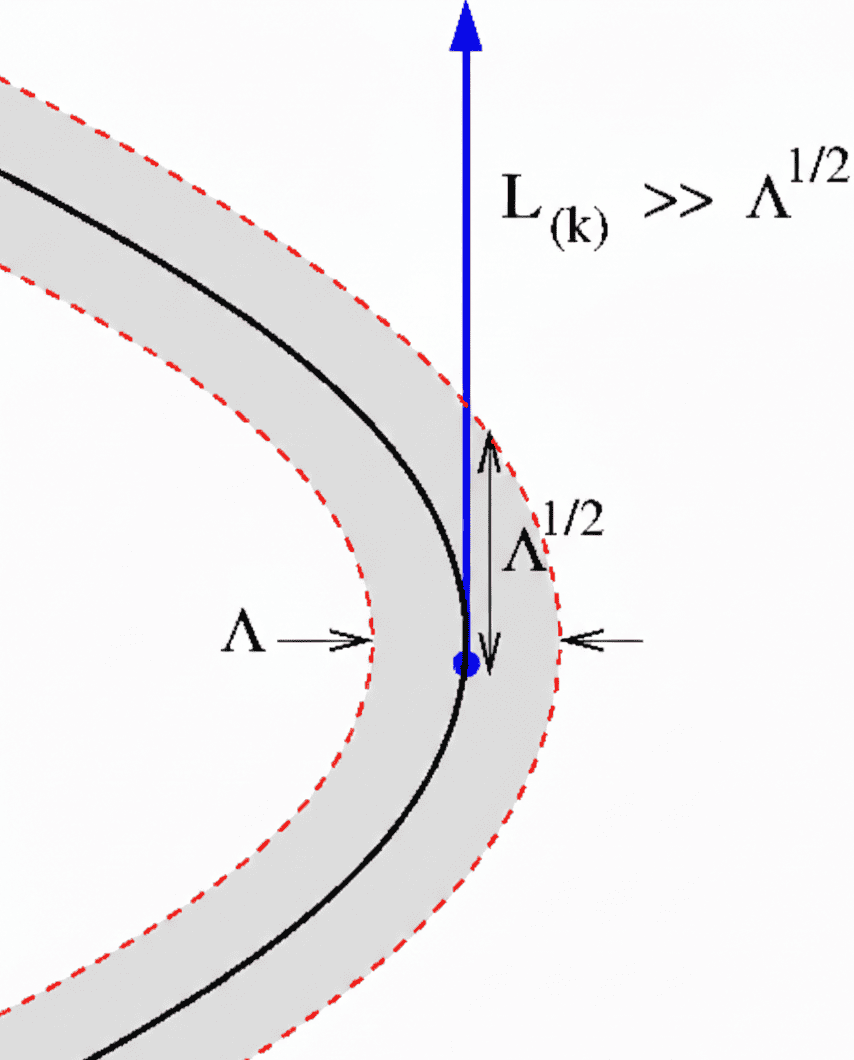
\includegraphics[width  =0.275 \textwidth]{crossover.png}}
\caption{(a) As the high-energy modes away from the FS are integrated 
out, the ratio $k_F/\Lambda$ grows, where $k_F$ denotes the size of the 
FS and $\Lambda$ is the energy cutoff perpendicular to it. 
For $m > 1$, the Green's functions develop singularities in the 
$k_F/\Lambda \rightarrow \infty$ limit, and it is precisely this behavior 
that gives rise to the UV/IR mixing of energy scales. (b) A two-dimensional slice of an $m$-dimensional FS. The 
typical momentum carried by a boson is proportional to 
$\tilde{\alpha}^{1/3}\, \Lambda^{\frac{d-m}{3}} \sim \tilde{e}^{\frac{1}{m+1}} 
\left({k_F}/{\Lambda}\right)^{\frac{m-1}{2(m+1)}} \Lambda^{1/2}$. 
For $m > 1$, this momentum greatly exceeds $\Lambda^{1/2}$ in the 
low-energy limit. Consequently, the momentum transferred by a boson is 
large enough to carry a fermion near the FS well outside the 
thin shell of width $\sim \Lambda$, leading to a suppression of virtual 
particle-hole excitations by powers of $\Lambda/k_F$ for $m > 1$.}\label{fig:FS2}
\end{figure}
%%%%%%%%%%%%%%%%%%

In order to control the Yukawa-like coupling between the fermions and 
bosons, and the strength of the UV/IR mixing, independently of one 
another, we tune both $d$ \cite{Chakravarty,Fit,Torroba} and $m$ 
\cite{senshank,Lee-Dalid,shouvik2}. To maintain the analyticity of the 
theory in momentum space --- which is equivalent to locality in real 
space --- for generic values of $m$, we introduce a two-component 
spinor~\cite{Lee-Dalid,shouvik2},
\begin{align}
\Psi_j^T(k) = \begin{bmatrix} \psi_{+,\lambda}(k) & \quad 
\psi_{-,\lambda}^\dagger(-k) \end{bmatrix},
\end{align}
and use it to formulate an action embedded in a $d$-dimensional momentum 
space, which takes the form of
%%%%%%%%%%%%%%%%%%%%
\begin{align}
\label{eqactphys}
S  &=   \sum_\lambda \int dk \,\bar \Psi_j(k)\,i
\Bigl[ 
{\vec \Gamma} \cdot {\vec K }  + \gamma_{d-m} \, \delta_k \Bigr] \Psi_{j}(k) \,
 e^{ \frac{{{\vec{L}}_{(k)}^2} } {\mu \, {\tilde{k}}_F} }
+ \frac{1}{2} \int  dk \,{\vec{L}}_{(k)}^2\,  \phi(-k) \, \phi(k) 
\nonumber\\ &\quad
 +     \frac{i \, e \, \mu^{x_e/2} }{\sqrt{N}}  \sum_\lambda  
\int dk dq  \,
\phi(q) \, \bar \Psi_{j}(k+q)\,  \gamma_{d-m} \Psi_{j}(k) \,.
%%%%%%%%%%
%\quad \delta_k =  k_{d-m}+ {\vec{L}}_{(k)}^2\,.
\end{align}
%%%%%%%%%%%%%%%%%
Here, $\vec{K} \equiv \{k_0, k_1, \ldots, k_{d-m-1}\}$ collects the 
frequency and the first $(d-m-1)$ components of the $d$-dimensional 
momentum vector, while $\vec{L}_{(k)} \equiv \{k_{d-m+1}, \ldots, k_d\}$ 
and $\delta_k = k_{d-m} + \vec{L}_{(k)}^2$. Within the $d$-dimensional 
momentum space, the components $\{k_1, \ldots, k_{d-m}\}$ and 
$\vec{L}_{(k)}$ represent the $(d-m)$ and $m$ directions perpendicular 
and parallel to the FS, respectively. The vector $\vec{\Gamma} \equiv 
\{\gamma_0, \gamma_1, \ldots, \gamma_{d-m-1}\}$ collects the gamma-matrices 
associated with $\vec{K}$. Since we are interested in co-dimensions 
satisfying $1 \leq d - m \leq 2$, it suffices to work with $2 \times 2$ 
gamma-matrices, for which we take $\gamma_0 = \sigma_y$, 
$\gamma_{d-m} = \sigma_x$, and define $\bar{\Psi} \equiv \Psi^\dagger \gamma_0$.

The leading terms in the non-interacting part of Eq.~\eqref{eqactphys} 
are invariant under the following rescaling transformations, expressed 
in terms of a mass scale $\mu$:
%%%%%%%%%%%%%%%%%%%%%%%%%%%%%%
\begin{align*}
\vec K & = \mu \,{\vec K'} \,, \quad k_{d-m} = \mu \, k_{d-m}' \,,
\quad {\vec{L}}_{(k)} = \sqrt{\mu} \;{\vec{L}}_{(k)}'  \,, \nn
\Psi_j (k) & =  \mu^{ -\,\frac{2 \,d + 4-m}{4}} \,\Psi'_j (k') \,, \quad 
\phi (k) = \mu^{ -\,\frac{2 \,d + 4-m}{4}} \, \phi'(k')\,. 
 \end{align*}
%%%%%%%%%%%%%%%%%%%%%% 
In the quadratic action of the boson, only the term $\vec{L}_{(k)}^2 \, 
\phi^*(k)\phi(k)$ is retained, because $|\vec{K}|^2 + k_{d-m}^2$ is 
irrelevant under the scaling in which each of $\{k_0, k_1, \ldots, 
k_{d-m}\}$ carries dimension $1$ and each of $\{k_{d-m+1}, \ldots, k_d\}$ 
carries dimension $1/2$. Put differently, the bosonic dynamics is so 
strongly dressed by particle-hole excitations that portions of the bare 
kinetic term become unimportant in the infrared. While the $(m+1)$-dimensional 
rotational symmetry of the bosonic action would naively place all of 
$\{k_{d-m}, \ldots, k_d\}$ on equal footing, the coupling to the fermions 
singles out $k_{d-m}$: the bosons that contribute most to fermionic 
scattering around $\pm K^*$ carry momenta satisfying $|\vec{L}_{(k)}| \gg 
k_{d-m}$, and so the dependence on $k_{d-m}$ in the bosonic kinetic term 
can be safely neglected when describing the fermionic dynamics in that 
region. Finally, $c_\parallel$ has been absorbed into a redefinition of 
the field.

The scaling dimension of the Yukawa-like coupling constant $e_0 = e\,\mu^{x_e/2}$ 
is $x_e/2$, where $x_e = 2 + m/2 - d$. By writing $e_0 = e\,\mu^{x_e/2}$, 
where $\mu$ is a mass scale, the coupling $e$ is rendered conveniently 
dimensionless. We further define $\tilde{k}_F = k_F/\mu$ as the 
dimensionless counterpart of $k_F$. The spinor carries an energy dispersion 
with two bands, $E_k = \pm\sqrt{\sum_{j=1}^{d-m-1} k_j^2 + \delta_k^2}$, 
which gives rise to an $m$-dimensional FS embedded in a $d$-dimensional 
momentum space, defined by the $d-m$ conditions $k_i = 0$ for 
$i \in \{1, \ldots, d-m-1\}$ and $k_{d-m} = -\vec{L}_{(k)}^2$.

Apart from $k_F$, which sets the size of the FS, the theory implicitly 
carries a UV cutoff $\Lambda$ for $\vec{K}$ and $k_{d-m}$. It is natural 
to identify $\Lambda = \mu$, which sets the largest energy --- or 
equivalently, the largest momentum perpendicular to the FS --- that 
fermions may carry. If $k_e$ denotes the typical energy scale at which 
one wishes to probe the system, the regime of interest is $k_e \ll 
\Lambda \ll k_F$. We study the RG flows of the two dimensionless 
parameters $e$ and $\tilde{k}_F$, generated by varying $\Lambda$ while 
requiring that low-energy observables remain independent of it. This is 
equivalent to the Wilsonian procedure of coarse-graining, in which 
high-energy modes away from the FS are integrated out at each step. 
Since the zero-energy modes are never integrated out, the ratio 
$k_F/\Lambda$ grows monotonically throughout the coarse-graining 
procedure. We therefore treat $k_F$ as a dimensionful coupling constant 
that flows to infinity in the low-energy limit --- a fact that captures, 
physically, the divergence of the FS size measured in units of the 
thickness of the thin shell surrounding it, as illustrated in 
Fig.~\ref{fig:FS2}(a).


%%%%%%%%%%%%%%%%%%%%%%%%%%%%
\section{Dimensional Regularization}
\label{dr}

%%%%%%%%%%%%%%%%%%%%%%%
\begin{figure}[t!]
\begin{center}
\subfigure[]{\includegraphics[width=0.3 \textwidth]{bos}}
\subfigure[]{\includegraphics[width=0.33 \textwidth]{fermi}} 
\subfigure[]{\includegraphics[width=0.3 \textwidth]{vert}} 
\end{center}
\caption{The one-loop diagrams for the (a) bosonic self-energy, (b) fermionic 
self-energy, and (c) vertex correction. In (a), the gray wiggly curve 
denotes the bare bosonic propagator. The solid arrows represent bare 
fermionic propagators, while the wiggly curves in (b) and (c) denote 
dressed bosonic propagators that incorporate the one-loop self-energy 
shown in (a).}\label{fig1loop}
\end{figure}
%%%%%%%%%%%%%%%%

For a given $m$, we tune $d$ towards the critical dimension, $d_c$, which defines the value of $d$ at which the one-loop quantum corrections diverge logarithmically in $\Lambda$, where $\Lambda \ll k_F$. Clearly, $x_e$ vanishes when $ {\tilde d}_c (m) = 2 + m / {2} $ and, in general, it will turn out that $ {\tilde d}_c \neq d_c$ for $1 <m < 2$.
This mismatch is a sign that $k_F$ enters the low-energy physics in a way that is singular in the large $k_F$ limit, resulting in UV/IR mixing. In order to identify $d_c$, we consider the one-loop quantum corrections.
Since the bare bosonic propagator is independent of $\lbrace k_{0}, \cdots ,k_{d-m} \rbrace $, the loop integrations involving it are ill-defined, unless one resums a series of diagrams that provides a non-trivial dispersion along those directions.
This amounts to rearranging the perturbative expansion such that the one-loop bosonic self-energy [cf. Fig.~\ref{fig1loop}(a)],
$ \Pi_1 (k) = -\, (i\,e)^2\, \mu^{x_e}
\int dq \, \text{Tr}
\left[ \gamma_{d-m} \,G_0 (k+q)\,\gamma_{d-m} \, G_0 (q) \right] $, is included at the `zero'-th order. Our unusual ordering of including Feynman diagrams, which is not organized by the number of loops, is forced upon us by the dynamical structure of the theory. Nevertheless, we adopt a systematic procedure which guarantees that every Feynman diagram is
included once and only once order by order in $\epsilon \equiv d_c - d_p$.




The dressed boson propagator is the one which includes the one-loop self-energy and is expressed as
\begin{align}
\label{eqbabos}
D_1(k) &= \left[ {\vec{L}}_{(k)}^2 - \Pi_1 (k) \right]^{-1} ,\quad
\Pi_1 (k)  = -\,\beta_{d} \, e^2 \, \mu^{x_e}
\frac{ ( \mu \, {\tilde{k}}_F )^{ \frac{m-1}{2}}  \, |\vec K|^{d-m}}{ |\vec{L}_{(k)}| }  \,,
%%%%%%%%%
\nn \beta_d & = \frac{  \Gamma^2 (\frac{d-m+1} {2})} {2^{\frac{2d+m-1}{2}} \, \pi^{\frac{d-1}{2}}  
| \cos \lbrace  \frac{\pi (d-m+1)} {2} \rbrace | \,  \Gamma(\frac{d-m}{2}) \Gamma (d-m+1)}\,,
\end{align}
to the leading order in $k/k_F$, for $|\vec K|^2/|\vec L_{(k)}|^2, ~\delta_k^2/|\vec L_{(k)}|^2 \ll k_F$. The constant $\beta_d$ is finite for $2 \leq d < 3$. Since $D_1(k)$ 
depends on $e$, the higher-loop diagrams are not accompanied by powers 
of $e^2$, but rather by powers of $\tilde{e} = e^{fr}$, where $fr$ is 
a fractional exponent \cite{Lee-Dalid}. The nonanalyticity of the 
exponent in the definition of the effective coupling signals that part 
of the quantum effects of the bosonic self-energy have been incorporated 
nonperturbatively through a resummation of the loop diagrams. It is worth 
emphasizing that $-\Pi_1(k)$ is the celebrated \textit{Landau-damping} 
term, which gives rise to the characteristic $\text{sgn}(k_0)\,|k_0|^{2/3}$ 
dependence of the fermionic self-energy --- a hallmark of NFL behaviour 
across a wide range of quantum critical systems 
\cite{max-isn, max-sdw, Lee-Dalid, ips-uv-ir1, ips-uv-ir2, ips-fflo, ips-2kf, ips-cavity}.
Furthermore, $D_1(k)$ diverges for $m > 1$ in the $k_F \rightarrow \infty$ 
limit. This reflects the fact that Landau-damping grows stronger as the 
FS becomes larger when $m > 1$, since a boson can then decay into 
particle-hole excitations spread across the entire FS. This stands in 
sharp contrast to the $m = 1$ case, where a low-energy boson with a given 
momentum can only decay into particle-hole excitations near isolated patches 
whose tangents are (anti)parallel to its momentum. For $m = 1$ and $m = 2$, $k_F$ drops out of Eq.~\eqref{eqbabos}, 
signaling the absence of UV/IR mixing. We note that Eq.~\eqref{eqbabos} 
is valid only when at least one direction remains tangential to the FS, 
and should therefore not be extended to $m < 1$, where conventional QFT 
methods apply without difficulty. In what follows, we restrict our 
attention to $m > 1$.

The apparent breakdown of the spatial rotational symmetry in the space spanned by the momentum coordinates, 
$\{k_{d-m}, \ldots, k_d\}$, [ cf. Eq.~\eqref{eqbabos}] is an artifact of 
the fact that the expression is valid only for bosons whose momentum is 
nearly tangential to the FS at $\pm K^*$. For a boson propagator with 
a generic momentum, $|\vec{L}_{(k)}|$ in Eq.~\eqref{eqbabos} should 
be replaced by $\sqrt{k_{d-m}^2 + \cdots + k_d^2}$, as required by the 
$(m+1)$-dimensional rotational symmetry. This is because, for any given 
boson momentum $k$, one can always find a point on the FS where $k$ is 
the local tangent. Choosing a coordinate system in which $k_{d-m} = 0$, 
the bosonic self-energy takes exactly the same form as in 
Eq.~\eqref{eqbabos}, and since this holds for any $k$, a generic boson 
propagator must be independent of the direction within the subspace 
spanned by $\{k_{d-m}, \ldots, k_d\}$. In what follows, we work with 
the expression in Eq.~\eqref{eqbabos}, since we are primarily interested 
in the physics near $\pm K^*$ on the FS. The bosons that couple most 
strongly to those two regions carry momenta satisfying $k_{d-m} \ll 
|\vec{L}_{(k)}|$, so that $\sqrt{k_{d-m}^2 + \cdots + k_d^2}$ reduces 
to $|\vec{L}_{(k)}|$ to good approximation. 

Incorporating the dressed bosonic propagator, $D_1$, the one-loop fermionic self-energy, $\Sigma_1 (q)$, needs to be computed, which is shown in Fig.~\ref{fig1loop}(b). An explicit computation leads to~\cite{ips-uv-ir1}
%%%%%%%%%%%%%%%%%%%%%%
\begin{align}
\Sigma_1 (q) &= \frac{(i\,e)^2  \, \mu^{x_e}}  {N} 
\int dk \,\gamma_{d-m} \, G_0 (q-k)\, \gamma_{d-m} \,D_1 (k) \nn
%%%%%%%%%%%%%%%
& = \frac{ -\,i \, e^{2\,(m+1)/3} \, \mu^{ x_e \, (m+1)/3} \, \vec \Gamma \cdot \vec Q    }
{ 6\, N \,   \pi^{(m-1)/2}
(4 \pi)^{\frac{d-m}{2}} \,2^{m-1} \,  | \sin \lbrace (m+1) \pi/3 \rbrace |\, 
 \beta_{d}^{(2-m)/3}  \,( \mu \, {\tilde{k}}_F )^{(m-1)(2-m)/6} }  \nn
& \; \quad \times \frac{  \Gamma ( \frac{3-  (m+1)(d-m) }{6}) \, 
\Gamma (  \frac{d-m-2 \beta}{2}) \,  \Gamma (  \frac{d-m+1}{2})  } 
{  \Gamma{(m/2)} \, \Gamma(\beta) \,  \Gamma ( d-m -  \beta + \frac{1}{2})
\, (\vec Q ^2)^{  \frac{3-  (m+1)(d-m) }{6}} } \,,
\label{eqsigma1}
\end{align} 
where  $\beta \equiv  {(d-m) \,(2-m)}/ {6}$. $\Sigma_1 (q)$ shows a logarithmic divergence
in the IR-scale $\Lambda$ at $ d_c(m) = m + {3}/(m+1) $. The value of $ d_c(m) $ is clearly smaller than ${\tilde d}_c$ within the range $1 <m<2$.
Setting $d=d_c(m) - \epsilon$, the divergence $\sim \ln \Lambda $
corresponds to the divergence captured by the pole, $1/\epsilon$, when translated into the language of dimensional regularization. This can be seen by rewriting the fermionic self-energy as
%%%%%%%%%%%
\begin{align}
\Sigma_1 (q) &= 
\left [ -\, \frac{e^{2 \,(m+1 ) /3}  } {{\tilde{k}}_F ^{ \frac{(m-1) (2-m)} {6}} \,N} 
\frac{u_1}{\epsilon}  + \text{ finite terms}
\right ] \left(i \, \vec \Gamma \cdot \vec Q \right ) ,\nonumber \\
%%%%%%%%%%%%
u_1 &= \frac{ \left( \pi/\beta_d \right)^{\frac{2-m}{2}} }
{ (4 \pi)^{\frac{3}{2(m+1)}} 2^{m-1}  
\left | \sin \Big( \frac{(m+1) \pi} {3} \Big) \right |  }
\, \frac{  \Gamma\Big (  \frac{m+4}{2(m+1)} \Big )  } 
{  \Gamma \big (\frac{m}{2} \big)\, \Gamma \Big (\frac{2-m}{2(m+1)}\Big )
 \, \Gamma \Big(  \frac{2m+5}{2(m+1)} \Big) }\,,
\end{align}
keeping terms upto the leading order in $q/k_F$.
%%%%%%%%%%%%%%%%%%%%%%
The one-loop vertex correction is shown in the Feynman diagram of Fig.~\ref{fig1loop}(c). It vanishes identically, which can be traced back to the existence o aa Ward identity \cite{Lee-Dalid}. The key advantage of our formalism is that we can tune the value if $ m$ from $ 1$ to $ 2 $ with the help of the expansion-parameter $\epsilon$, which remains small as required. Thus, we achieve a controlled perturbative expansion through $\epsilon $, as long as we remain within $1 \leq m \leq 2 $. We would like to emphasize that we are tuning the two dimenionalities, namely, $m$ and $d$, independently, which of course must obey the constraint $m<d$ to make any physical sense. This allows us to tune $d$ such that $\epsilon =  d_c(m) - d $ is perturbatively small for a given $m$.


Eq.~\eqref{eqactphys} is taken to be the \textit{physical action}, 
defined at an energy scale $\mu \sim \Lambda$, and consists of the 
fundamental Lagrangian expressed in terms of non-divergent quantities. 
However, loop integrals generically produce divergent contributions, 
and to handle these we employ renormalization via dimensional 
regularization. The UV-divergent terms are those that arise in the 
$\epsilon \rightarrow 0$ limit. To systematically control these 
divergences, we work within the minimal subtraction ($\mathrm{MS}$) 
renormalization scheme \cite{thooft, weinberg}, in which the divergent 
parts of loop contributions are cancelled by adding appropriate 
counterterms. More precisely, we adopt the modified minimal subtraction 
($\overline{\mathrm{MS}}$) scheme, wherein one absorbs not only the 
strictly divergent pole but also the universal finite term proportional 
to $\epsilon^0$ that invariably accompanies the $1/\epsilon$ pole into 
the corresponding counterterm. 


The counterterm action, $S_{CT}$, which is designed to absorb all singular 
contributions, is constructed by introducing counterterm factors as power 
series $A_{\zeta} = \sum_{n=1}^\infty Z_{\zeta,n}/\epsilon^n$ with 
$\zeta \in [1,4]$, chosen so as to cancel the divergent $1/\epsilon^n$ 
contributions from the Feynman diagrams. It takes the form of
%%%%%%%%%%%%%%%%%%%%
\begin{align}
\label{actcount}
S_{CT}  &=   \sum_\lambda \int dk \,\bar \Psi_\lambda (k)\, i
\Bigl[ A_1 \, {\vec \Gamma} \cdot {\vec K } 
+ A_2 \, \gamma_{d-m} \, \delta_k \Bigr] \Psi_\lambda (k) \,
 e^{ \frac{{{\vec{L}}_{(k)}^2} } {\mu \, {\tilde{k}}_F} }
%%%%%%%
\nn & \quad + \frac{A_3}{2} \int  dk \,{\vec{L}}_{(k)}^2\,  \phi(-k) \, \phi(k) 
\nonumber\\ &\quad
 +   \frac{i \, e \, \mu^{x_e/2} }{\sqrt{N}}  \sum_\lambda  
\int dk dq  \,A_4 \,\phi(q) \, \bar \Psi_\lambda (k+q)\,  \gamma_{d-m} \Psi_\lambda (k) \,.
\end{align}
%%%%%%%%%%%%%%%%%
Due to the $(d-1)$-dimensional rotational invariance in the space 
perpendicular to the FS, each term in $\vec{\Gamma} \cdot \vec{K}$ is 
renormalized in the same way. A Ward identity enforces $A_4 = A_3$ 
\cite{Lee-Dalid}. Subtracting $S_{CT}$ from the so-called \textit{bare} 
action $S_{\text{bare}}$, we obtain the renormalized action, which 
serves as the \textit{physical} effective action of the theory, 
rewritten entirely in terms of non-divergent quantum parameters. Here,
%%%%%%%%%%%%%%%%%%%%%%%%
\begin{align}
\label{act7}
S_{\text{bare}} & =   \sum_\lambda \int d k_B
\, \bar \Psi_{B \lambda }(k_B) \, i
\Bigl[  \vec \Gamma \cdot \vec K_B +  \gamma_{d-m} \delta_{k_B}  \Bigr] 
\Psi_{B \lambda }(k_B) \, \exp \Big \lbrace \frac {{\vec{L}}_{(k),B}^2}  {  k_{F,B} } \Big \rbrace
\nonumber\\
&\quad +\frac{1}{2} \int  d k_B \,
 {\vec{L}}_{(k)}^2\,  \phi_B(-k_B) \, \phi_B(k_B) \nonumber \\
 & \quad +     \frac{i \, e_B }{\sqrt{N}}  \sum_\lambda  
\int d k_B \, d q_B \,\phi_B(q_B) \, \bar \Psi_{B \lambda }(k_B+q_B) 
\, \gamma_{d-m} \Psi_{B \lambda }(k_B) \, ,
\end{align}
%%%%%%%%%%%%
consisting of the \textit{bare quantities}, each labelled with the subscript ``$B$''.
While the bare parameters may be divergent, the physical observables 
are identified with the renormalized coupling constants, which evolve 
as functions of the logarithm of the floating energy scale 
$\mu = \mu_0\,e^{-l}$. We now relate the bare quantities to their 
renormalized counterparts --- written without the superscript ``$B$'' 
--- via the multiplicative $Z_\zeta$-factors, such that
$S_{\text{bare}}  =  S + S_{CT}$ and $ Z_{\zeta}  =  1 + A_{\zeta}$.
%%%%%%%%%%%%%%%%%%%
Here,
\begin{align*}
& \vec K = \frac{Z_2}{Z_1}\, \vec K_B \, , \quad k_{d-m} = k_{B, d-m} \, , 
\; {\vec{L}}_{(k)} = {\vec{L}}_{(k), B} \,, 
\; \Psi(k)  =  \frac{\Psi_B(k_B) } {\sqrt{ Z_\Psi}}\,, 
\;   k_F =\mu \, {\tilde{k}}_F\,,
%%%%%%%%%%
\nn & \phi(k) = \frac{ \phi_B(k_B)}  { \sqrt{Z_\phi} }\,, \;
e_B  =  \frac{1} {\sqrt{Z_3}} 
\left( \frac{Z_2}{Z_1} \right)^{\frac{d-m} {2} } \mu^{ \frac{x_e} {2} }  e\,,
%%%%%%%%%%
\nn & Z_\Psi =  Z_2 \left( \frac{Z_2}{Z_1} \right)^{d-m}, \;
Z_\phi = Z_3 \left( \frac{Z_2}{Z_1} \right)^{d-m}.
\end{align*}
%%%%%%%%%%%%%%
Restricting to the one-loop order, we have $Z_\zeta = 1 + \frac{Z_{\zeta,1}}{\epsilon}$, with
\begin{align}
 Z_{1,1} = - \,e^{ 2\, (m+1 ) /3}  \, u_1  /\big [ {\tilde{k}}_F^{ \frac{(m-1)\, (2-m)} {6}} \,N  \big ] 
\text{ and } Z_{2,1}  = Z_{3,1} = Z_{4,1} =  0 \,.
\end{align}


In the language of Renormalization Group (RG) transformations, the beta-function of a coupling-constant $g$ is defined as $\beta_g = \partial_{\ln \mu} g = \mu\, \partial_\mu g \equiv \partial_l g$. As we integrate out energy-shells, $\beta_g$ is the function that determines the flow of $g$ with $\ln \mu$. At one-loop level, for the two coupling-constants, $\tilde k_F$ and $e$, the beta-functions take the forms of
%%%%%%%%%%%%%%%%%%%%%%
\begin{align}
& \beta_{\tilde k_F}  = -\, \tilde k_F \,, \quad
\beta_e = 
 - \left[ \frac{\epsilon}{2} + \frac{(m-1) \, (2-m)}{4 \, (m+1)} \right]  e 
+ \frac{ u_1 \, {\tilde e} }{2 \, N} \, e \,,\nn 
%%%%%%%%%%%%%%%%%%%
& {\tilde e} \equiv \frac{e^{ 2 (m+1 ) /3}  } 
{{\tilde{k}}_F ^{ \frac{(m-1) \,(2-m)} {6}}} \,,\quad
z = 1 - \frac{\partial} {\partial {\ln \mu}} \left(\frac{Z_2} {Z_1}\right) ,\quad
\eta_\psi = \frac{\mu}{2} \, \frac{\partial {Z_\psi}} {\partial {\mu}} \,, \quad
\eta_\phi = \frac{\mu}{2} \, \frac{\partial {Z_\phi}} {\partial {\mu}}\,.
\label{eq:be}
\end{align}
%%%%
Here, $z$ is the dynamical critical exponent and $\eta_\psi$ ($\eta_\phi$) incorporates the anomalous dimension for the fermions (bosons). The quantity $\tilde{k}_F$ increases under the RG flow because the size 
of the FS, measured in units of $\mu$, grows at low energies. The first 
term in $\beta_e$ indicates that $e$ remains strictly relevant at 
$d = d_c(m)$ for $1 < m < 2$, as reflected by $x_e > 0$ and 
$\tilde{d}_c > d_c$. Intriguingly, the form of the loop correction --- 
the second term --- reveals that higher-order corrections are controlled 
not by $e$ itself, but by an effective coupling $\tilde{e}$, which is 
responsible for the $e^{fr}$ powers that accompany them, as discussed 
earlier. The beta-function for $\tilde{e}$, which no longer contains 
$\tilde{k}_F$, is given by
%%%%%%%%%%%%%%%%%%%
\begin{align}
\label{bstable}
 \beta_{\tilde e}   = -\, \frac{(m+1)\, \epsilon}{3} \, {\tilde e} 
+ \frac{ (m+1)\,  u_1} {3N} \, {\tilde e}^2 + \mathcal{O}({\tilde e}^3) \,.
\end{align}
%%%%%%%%%%%
From this, we see that $\tilde{e}$ flows to an IR-stable fixed point at 
$\tilde{e}^* = N\epsilon/u_1 + \mathcal{O}(\epsilon^2)$. For small 
$\epsilon$, this interacting fixed point is perturbatively accessible, 
despite the fact that the scaling dimension $x_e$ of the bare coupling 
$e$ remains positive in the $\epsilon \rightarrow 0$ limit for 
$1 < m < 2$. Although $e$ grows at low energies, this growth is 
compensated by the Landau damping, which also strengthens as the 
effective size of the FS increases. It is the competition between the 
interaction and the Landau damping that renders the effective coupling 
marginal at the true critical dimension $d_c$, which does not coincide 
with $\tilde{d}_c$ for $1 < m < 2$. We also observe that $k_F$ drops 
out of the effective coupling not only for $m = 1$ but also for $m = 2$. 
In the latter case, the $k_F$ dependence arising from the Landau damping 
is precisely cancelled by the $k_F$ dependence from the phase space of 
intermediate states in Fig.~\ref{fig1loop}(b). Nevertheless, UV/IR 
mixing persists for all $m > 1$, since the Landau damping diverges in 
the large-$k_F$ limit. Finally, the fixed-point values of $\{z, \eta_\psi, \eta_\phi\}$ 
evaluate at one-loop order to $z^* = 3/[3 - (m+1)\,\epsilon]$ and 
$\eta_\psi^* = \eta_\phi^* = -\epsilon/2$. It is remarkable that these 
exponents turn out to be insensitive to the details of the FS --- such 
as $\beta_d$ --- despite the fact that patch scaling is violated by 
$k_F$. This vindicates our use of the exponential cutoff scheme in 
Eq.~\eqref{eqkf}, which captures the compactness of the FS in a minimal 
way without requiring knowledge of its precise shape. The finite anomalous 
dimensions arise from a dynamical balance between the two strongly 
relevant couplings, $e$ and $k_F$ --- a mechanism that is qualitatively 
opposite to cases where finite anomalous dimensions emerge from a balance 
between two \textit{irrelevant couplings} \cite{shouvik2}.




%%%%%%%%%
\section{Renormalization-Group equations}
\label{secrg}

A renormalized Green's function, $G^{({n_\psi} ,{n_\psi} , {n_\phi} )}$, defined by the expectation value,
$$ \Bigl< \phi( k^{1} ) \cdots \phi(k^{{n_\phi} })\,
\Psi( k^{{n_\phi} +1} ) \cdots \Psi(k^{{n_\phi}+n_\psi })\,
 \bar \Psi( k^{n_{\phi}+n_\psi+1} )  \cdots \bar \Psi(k^{n_\phi+2 \,n_\psi} ) \Bigr> $$
 %%%%%%%%%%%%%%%%%
$ = G^{({n_\psi} ,{n_\psi} , {n_\phi} )}( \{ k^\alpha \}; \tilde e, \tilde k_F , \mu )$
$\delta^{d+1} \left( \sum_{\alpha =1}^{{n_\phi+n_\psi} } k^\alpha 
- \sum_{ \alpha^\prime ={n_\phi} + n_\psi +1}^{2 {n_\psi} + {n_\phi}} k^{ \alpha^\prime} \right)$,
is the one which satisfies the RG equation. This is expressed as
%%&&%%%%%%%%%%%%%
\begin{align}
& \Bigg [
- \sum_{ \alpha=1}^{2 \,{n_\psi}  + {n_\phi} } \left(
z \, \vec K^\alpha \cdot \nabla_{K^\alpha}
+ k^{\alpha^\prime}_{d-m} \, \partial_{k^{\alpha^\prime}_{d-m}}
+ \frac{ \vec{L}_{(k^\alpha)} } {2}   \cdot  \nabla_{{L}_{(k^\alpha)}}
\right)  
+ \beta_{\tilde k_F}  \partial_{\tilde k_F}
+ \beta_{\tilde e}  \partial_{\tilde e}
%% %%%%%%%%%%%%%%%%%
\nn & \quad + 2  \, {n_\psi}  \left ( -  \frac{2 \, d_c - 2 \, \epsilon + 4 -m }{4} +  \eta_\psi \right)   
%%%%%%%%%%%%
 +  {n_\phi} \left ( -  \frac{2 \, d_c - 2 \, \epsilon +4 -m }{4} +  \eta_\phi \right) 
+  d_c - \epsilon \nn & \quad
%%%%%%%%%%%%%
 + 1 - \frac{m}{2}  + (d_c - \epsilon - m)\, (z-1)
\Bigg ]
\, G^{({n_\psi} , {n_\psi}  ,{n_\phi})}(\{ k_i \}; {\tilde e}, \tilde k_F , \mu ) 
= 0 \,.
\label{RGeq}
\end{align}
%%%%%%%%%%%%%%%%%
A generic $G^{({n_\psi} ,{n_\psi} , {n_\phi} )}$ contains both fermionc and bosonic fields. In particular, we are interested in the two-point functions for the bosons and the fermions because they contain the information of the generic scaling-form at the IR fixed point. These are:
\begin{align}
\label{Dk0}
G^{(0,0,2)} &=  \frac{1}{ \left (  \vec{L}_{(k)}^2 \right )^{ 2 \Delta_\phi } } \,
f_F \left( 
\frac{| \vec K |^{1/z^*} }{  \vec{L}_{(k)}^2 } ,  \frac{k_{d-m} }{k_F} ,  
\frac{  \vec{L}_{(k)}^2 } {k_F}
\right),   \nn
G^{(1,1,0)} & =   \frac{1}{ | \delta_k |^{ 2 \Delta_\psi} } \,
f_B \left( \frac{ | \vec K |^{1/z^*} }{\delta_k} , \frac{\delta_k }{k_F} ,  \frac{  \vec{L}_{(k)}^2 } {k_F}
 \right) , 
\end{align}
where 
$2 \,\Delta_\phi = 1 - (z^*-1) \left (\frac{3}{m+1}-\epsilon \right) - 2 \,\eta^*_\phi = 1+O(\epsilon^2)$ and
$2\, \Delta_\psi = 1 - (z^*-1) \left (\frac{3}{m+1}-\epsilon \right) - 2 \,\eta^*_\psi = 1+O(\epsilon^2)$.
From the expressions at one-loop order, we infer the universal scaling-forms to be
%%%%%%%%%%%%%%%%%%%%%%%%%%%%
\begin{align}
& f_B( X,Y,Z)  =  \left[1 + \beta_d \, {\tilde e}^{\frac{3}{m+1}}
X^{\frac{3}{m+1} }
Z^{-\frac{3(m-1)}{2(m+1)}}
\right]^{-1}, \nn &
f_F( X,Y,Z)  =  -i \left[ C \, ( {\vec  \Gamma} \cdot \hat {\vec K} ) \, X   + \gamma_{d-m} \right]^{-1} ,
%%%%%%%
C = \mu^{ \frac {m+1}{3} \epsilon  } \left [
1 - \frac{(m+1) \, \gamma \, \epsilon } {6}
\right ],
\end{align}
in the limit $ Y, Z \rightarrow 0$ with $X$ held fixed. 
The expressions show that $f_D$ has a singular dependence on $ Z $ 
in the $ Z\rightarrow 0$ limit. We notice that the sliding symmetry being absent for the momentum coordinates of $\delta_k$ and $\vec L_{(k)}$,
the fermionic Green's function's dependence on $\delta_k$ and $\vec L_{(k)}$ is distinct in general.

%%%%%%%%%%%%%%%
\section{Physical relevance of the expansion-parameter $\epsilon $}
\label{dimexp}

The motivation for employing dimensional regularization and, ultimately, 
the small-$\epsilon$ expansion is to shed light on the stark difference 
in the characteristics of NFLs with $d_p = 2$ and $d_p = 3$. Since the 
former has an $m = 1$ FS, $k_F$ plays no role in the low-energy scaling. 
By contrast, $k_F$ enters as an important scale for $d_p = 3$ NFLs 
precisely due to UV/IR mixing. We now examine how this transition occurs 
in a systematic way by tuning $d$ and $m$ continuously. Although systems 
with non-integer dimensions are unphysical in their own right, they 
provide valuable insight into how $d$ and $m$ each contribute to the 
distinct properties of metals in actual physical dimensions.

For $d_p = 3$, one has $m = 2$, and $k_F$ is seen to drop out of the 
expression for $\tilde{e}$. Nevertheless, the intrinsic UV/IR mixing 
still manifests itself in the dispersion relations of the fermion and 
boson, which go as $k_0 \sim k_x + \vec{L}_{(k)}^2$ and 
$k_0 \sim \vec{L}_{(k)}^3$, respectively, up to small corrections. 
These two fields can have different effective dynamical critical exponents 
at the scale-invariant fixed point, with the mismatch compensated by 
$k_F$. Our analysis therefore yields the correct scaling behavior, 
consistent simultaneously for both bosons and fermions, by incorporating 
the dimensional parameter $k_F$ in an appropriate way. This stands in 
contrast to the $m = 1$ case, where the dispersions of bosons and 
fermions obey the same scaling behavior \cite{Lee-Dalid}. UV/IR mixing 
also plays an important role in suppressing higher-loop quantum 
corrections for $m > 1$, a point we turn to in the next section.



%%%%%%%%%%%%%
\section{Higher-Loop Diagrams And Expansion Parameter}
\label{secexp}

In Ref.~\cite{Lee-Dalid}, the $d_p = 2$ case was treated, where the 
two- and three-loop Feynman diagrams were shown to be suppressed by positive 
powers of $\tilde{e}$, with $\tilde{e} = \mathcal{O}(\epsilon)$. A 
general argument also exists outlining why higher-loop diagrams are 
systematically suppressed by successively higher powers of $\tilde{e}$. 
Our systematic expansion in $\epsilon$ is distinct from an expansion in 
powers of $1/N$, and does not suffer from the proliferation of planar 
diagrams that afflicts the $1/N$ expansion \cite{SSLee-largeN, max-sdw}. 
The introduction of extra codimensions mathematically suppresses the 
density of states at low energies, thereby reducing quantum fluctuations. 
This results in a weaker infrared singularity, which in turn permits a 
controlled expansion for sufficiently small $\epsilon$. We have generalized the treatment of Ref.~\cite{Lee-Dalid} to $d_p > 2$, 
where consequently $m > 1$. While the suppression of higher-loop diagrams 
by positive powers of $\tilde{e}$ persists unchanged for $m > 1$, a 
qualitatively new feature emerges: the explicit appearance of an 
additional energy-scale in the form of $k_F$.


To make an estimate of the magnitude of higher-loop corrections, we first discuss 
an interplay between $k_F$ and $\Lambda$ that plays an important role 
for $m > 1$. Let $k = \{\mathbf{K}, k_{d-m}, \vec{L}_{(k)}\}$ denote 
the momentum flowing through a boson propagator within a two-loop or 
higher-loop diagram. When $|\mathbf{K}|$ is of order $\Lambda$, the 
typical momentum carried by the boson along the tangential direction of 
the FS is given by $|\vec{L}_{(k)}|^3 \sim \tilde{\alpha}\,\Lambda^{d-m}$, 
where $\tilde{\alpha} = \beta_d\,e^2\,\mu^{x_e}\,(\mu\,\tilde{k}_F)^{(m-1)/2}$ 
[cf.\ Eq.~\eqref{eqbabos}]. When $(\tilde{\alpha}\,\Lambda^{d-m})^{1/3} 
\gg \sqrt{\Lambda}$, the momentum imparted from the boson to the fermion 
greatly exceeds $\sqrt{\Lambda}$, as illustrated in Fig.~\ref{fig:FS2}(b). 
Physically, this means that the typical energy of virtual particle-hole 
excitations within the loop is much larger than $\Lambda$, and as a 
result the loop contributions are suppressed by a power of $\Lambda/k_F$ 
at low energies. By contrast, no such suppression arises when 
$(\tilde{\alpha}\,\Lambda^{d-m})^{1/3} \ll \sqrt{\Lambda}$. The 
crossover between these two regimes is controlled by the dimensionless 
quantity $\lambda_{\text{cross}} \equiv \tilde{e}^2(k_F/\Lambda)^{m-1}$, 
which determines whether $(\tilde{\alpha}\,\Lambda^{d-m})^{1/3}$ is 
much greater or much less than $\Lambda^{1/2}$.

For $m = 1$, the $k_F$ dependence drops out entirely, including from 
the higher-loop diagrams. Since $\tilde{e} \sim \mathcal{O}(\epsilon)$ 
within the perturbative window, one always operates in the limit 
$\lambda_{\text{cross}} \ll 1$ for $m = 1$. The situation is 
qualitatively different for $m > 1$, where the tangential momentum 
carried by the boson depends on both $\Lambda$ and $k_F$. Indeed, for 
a fixed value of $\tilde{e} \sim \mathcal{O}(\epsilon)$, one is always 
driven into the regime $\lambda_{\text{cross}} \gg 1$ for $m > 1$ at 
sufficiently low energies, since $k_F$ carries a positive scaling 
dimension and $k_F/\Lambda$ flows to infinity in the low-energy limit. 
The crossover occurs at the energy scale $\Lambda \sim 
\tilde{e}^{2/(m-1)}\,k_F$. It is worth noting that for small $\epsilon$ 
and $(m-1)$, there exists a wide energy window before the theory enters 
the low-energy regime controlled by $\lambda_{\text{cross}} \gg 1$. In 
this strictly low-energy limit, higher-loop diagrams are suppressed by 
$k_F$, as has also been pointed out in Ref.~\cite{schafer} for the 
specific case of $d_p = 3$ and $m = 2$.

For general $m > 1$ with $\lambda_{\text{cross}} \gg 1$, the two-loop 
bosonic and fermionic self-energies are given by \cite{ips-uv-ir1}
$$\Pi_2(k) \sim \frac{\tilde{e}^{\frac{m}{m+1}}}{k_F^{\frac{m-1}{2(m+1)}}} 
\frac{|\vec{K}|^{\frac{m}{m+1}}}{N\,|\vec{L}_{(k)}|}\,\Pi_1(q) 
\quad \text{and} \quad \Sigma_{2a}(k) \sim \tilde{e}^{\frac{2(m-1)}{m+1}} 
\left(\frac{\Lambda}{k_F}\right)^{\frac{2(m-1)}{m+1}} 
i\,\gamma_{d-m}\,\delta_k\,,$$
respectively, to leading order in $\Lambda/k_F$. The vertex correction 
is related to the fermionic self-energy through the Ward identity. 
Compared to the one-loop self-energies, the two-loop corrections are 
therefore suppressed not only by $\tilde{e}$ but also by powers of 
$\Lambda/k_F$. Owing to this suppression by $1/k_F$, no logarithmic 
or higher-order divergence appears at the critical dimension, and 
consequently the critical exponents receive no corrections from the 
two-loop diagrams in the $k_F \rightarrow \infty$ limit. The suppression 
by $\Lambda/k_F$ can be traced back to the large Landau damping, which 
quenches quantum fluctuations at low energies. Since this mechanism is 
not specific to the two-loop diagrams, we expect all higher-loop 
contributions to be suppressed by $\tilde{e}$ and $1/k_F$ in the 
low-energy limit --- a conclusion we have verified explicitly for the Aslamazov-Larkin-type
diagrams comprising three loops.


%%%%%%%%%%%%%
\section{Outlook}
\label{conclusion}

In this chapter, we have demonstrated how to extract the scaling behaviour of NFLs  with a FS of general dimensions and co-dimensions, using a dimensional regularization scheme.  For $m>1$, the low-energy physics becomes sensitive to the size of FS, $k_F$, which results in an intriguing phenomenon of UV/IR mixing. By tuning the dimension below the upper critical dimension, we have shown that there exists a stable NFL fixed point where both interaction and UV/IR mixing play crucial roles.
We have also shown that the critical exponents at the low-energy fixed point are not modified by higher-loop diagrams for $m>1$. In ths next chapter, we will demonstrate how the Ising-nematic order parameter provides a ``stronger glue'' compared to phonons, bringing about unconventional superconductivity.


%\bibliographystyle{spphys.bst}
%\bibliography{ref.bib}

\begin{thebibliography}{10}
\providecommand{\url}[1]{{#1}}
\providecommand{\urlprefix}{URL }
\expandafter\ifx\csname urlstyle\endcsname\relax
  \providecommand{\doi}[1]{DOI \discretionary{}{}{}#1}\else
  \providecommand{\doi}{DOI \discretionary{}{}{}\begingroup
  \urlstyle{rm}\Url}\fi

\bibitem{sachdev_book}
S.~Sachdev, \emph{Quantum Phase Transitions}, 2nd edn. (Cambridge University
  Press, 2011)

\bibitem{Lee-Dalid}
D.~Dalidovich, S.S. Lee, Phys. Rev. B \textbf{88}, 245106 (2013).
\newblock \doi{10.1103/PhysRevB.88.245106}

\bibitem{lee-review}
S.S. Lee, Annu. Rev. Condens. Matter Phys. \textbf{9}, 227 (2018).
\newblock \doi{https://doi.org/10.1146/annurev-conmatphys-031016-025531}

\bibitem{ips-uv-ir1}
I.~Mandal, S.S. Lee, Phys. Rev. B \textbf{92}, 035141 (2015).
\newblock \doi{10.1103/PhysRevB.92.035141}

\bibitem{Shouvik1}
S.~Sur, S.S. Lee, Phys. Rev. B \textbf{90}, 045121 (2014).
\newblock \doi{10.1103/PhysRevB.90.045121}

\bibitem{LEE2008}
S.S. {Lee}, Phys. Rev. B \textbf{78}(8), 085129 (2008).
\newblock \doi{10.1103/PhysRevB.78.085129}

\bibitem{nayak}
C.~{Nayak}, F.~{Wilczek}, Nucl. Phys. B \textbf{430}, 534 (1994).
\newblock \doi{10.1016/0550-3213(94)90158-9}

\bibitem{mross}
D.F. Mross, J.~McGreevy, H.~Liu, T.~Senthil, Phys. Rev. B \textbf{82}, 045121
  (2010).
\newblock \doi{10.1103/PhysRevB.82.045121}

\bibitem{shouvik2}
S.~Sur, S.S. Lee, Phys. Rev. B \textbf{91}, 125136 (2015).
\newblock \doi{10.1103/PhysRevB.91.125136}

\bibitem{Fit}
A.L. Fitzpatrick, S.~Kachru, J.~Kaplan, S.~Raghu, Phys. Rev. B \textbf{88},
  125116 (2013).
\newblock \doi{10.1103/PhysRevB.88.125116}.
\newblock \urlprefix\url{http://link.aps.org/doi/10.1103/PhysRevB.88.125116}

\bibitem{Torroba}
G.~Torroba, H.~Wang, Phys. Rev. B \textbf{90}, 165144 (2014).
\newblock \doi{10.1103/PhysRevB.90.165144}.
\newblock \urlprefix\url{http://link.aps.org/doi/10.1103/PhysRevB.90.165144}

\bibitem{ips-sc}
I.~Mandal, Phys. Rev. B \textbf{94}, 115138 (2016).
\newblock \doi{10.1103/PhysRevB.94.115138}

\bibitem{Chakravarty}
S.~{Chakravarty}, R.E. {Norton}, O.F. {Sylju{\aa}sen}, Phys. Rev. Lett.
  \textbf{74}, 1423 (1995).
\newblock \doi{10.1103/PhysRevLett.74.1423}

\bibitem{senshank}
T.~Senthil, R.~Shankar, Phys. Rev. Lett. \textbf{102}, 046406 (2009).
\newblock \doi{10.1103/PhysRevLett.102.046406}

\bibitem{max-isn}
M.A. Metlitski, S.~Sachdev, Phys. Rev. B \textbf{82}, 075127 (2010).
\newblock \doi{10.1103/PhysRevB.82.075127}

\bibitem{max-sdw}
M.A. Metlitski, S.~Sachdev, Phys. Rev. B \textbf{82}, 075128 (2010).
\newblock \doi{10.1103/PhysRevB.82.075128}

\bibitem{ips-uv-ir2}
I.~Mandal, Eur. Phys. J. B \textbf{89}(12), 278 (2016).
\newblock \doi{10.1140/epjb/e2016-70509-4}

\bibitem{ips-fflo}
D.~Pimenov, I.~Mandal, F.~Piazza, M.~Punk, Phys. Rev. B \textbf{98}, 024510
  (2018).
\newblock \doi{10.1103/PhysRevB.98.024510}

\bibitem{ips-2kf}
I.~Mandal, Nucl. Phys. B \textbf{1005}, 116586 (2024).
\newblock \doi{10.1016/j.nuclphysb.2024.116586}

\bibitem{ips-cavity}
I.~{Mandal}, Ann. Phys. \textbf{474}, 169925 (2025).
\newblock \doi{10.1016/j.aop.2025.169925}

\bibitem{thooft}
G.~'t~Hooft, Nucl. Phys. B \textbf{61}, 455 (1973).
\newblock \doi{https://doi.org/10.1016/0550-3213(73)90376-3}

\bibitem{weinberg}
S.~Weinberg, Phys. Rev. D \textbf{8}, 3497 (1973).
\newblock \doi{10.1103/PhysRevD.8.3497}

\bibitem{SSLee-largeN}
S.S. Lee, Phys. Rev. B \textbf{80}, 165102 (2009).
\newblock \doi{10.1103/PhysRevB.80.165102}

\bibitem{schafer}
T.~Sch\"afer, K.~Schwenzer, Phys. Rev. D \textbf{70}, 054007 (2004).
\newblock \doi{10.1103/PhysRevD.70.054007}

\end{thebibliography}

%%%%%%%%%%%%%%%%%%%%%%%%%%%%%%%%%%%%%%%%%%%%%%%%%%%%%%%
\chapter{Enhancement Of Superconductivity By Ising-Nematic Order Parameter}
\label{chap-sc}


\abstract{This chapter demonstrates how  the techniques of dimensional regularization and renormalization-group 
(RG) are employed to investigate four-fermion interactions capable of inducing superconducting instabilities. The computations are carried out in the presence of Ising-nematic ordering, studied in the earlier chapter. The fermionic part is characterised by critical Fermi 
surfaces of generic dimensions ($m$) and co-dimensions ($d-m$). The superconducting 
instabilities are shown to be enhanced by the  fermionic quasiparticles' interactions with the gapless 
Ising-nematic order parameter. By analysing the RG-flow equations, the stable fixed points are identified as functions of $d$ and $m$. The results reveal that the flow toward a NFL fixed point is consistently preempted by 
Cooper-pair formation in the physical regimes of $(d=3, m=2)$ and 
$(d=2, m=1)$. Most importantly, the results demonstrate a significant 
enhancement of superconductivity driven by the order-parameter 
fluctuations.}


%%%%%%%%%%%%%%%%%%%%%%%%
\section{Introduction}

We continue our exploration of the Ising-nematic ordering \cite{Lee-Dalid, ips-uv-ir1} by examining 
its effect on a four-fermion interaction of strength $V$ in the pairing 
channel. Taking a system embedded in $d$ spatial dimensions (see Chapter 1)
possessing an $m$-dimensional Fermi surface (FS),
the tree-level scaling dimension of $V$ is $[V] = -d + 1 + m/2$. As we 
shall see, scatterings in the BCS channel are enhanced by powers of the 
FS volume, $\sim k_F^m$, so that the effective coupling governing the 
potential superconducting instability becomes $\tilde{V} = V\,k_F^{m/2}$, 
with an enhanced scaling dimension of $[\tilde V ] = -d + 1 + m$. This effective 
coupling is marginal precisely when the co-dimension takes the value 
$d - m = 1$. Our goal is to understand how the interactions between 
the fermions and the critical bosons conspire to enhance a pairing 
instability \cite{ips-sc}.


%%%%%%%%%%%%%%%%%%%%%
\section{Superconducting Instability}
\label{sec-sc-action}



To investigate the emergence of superconducting instabilities within the 
prescribed non-Fermi liquid framework, we augment the fermion-boson 
action introduced in Chapter 1 with the requisite four-fermion 
interaction terms. The following terms can give rise to Cooper pairing in the BCS channel:
\begin{align}
 & \int \left ( \prod_{s=1}^4 {dp_s }  \right)
  \frac{    \mathcal{F}(p_1,p_3;p_2,p_4)  }   { 4 } \, \Big [
 \big \lbrace \bar{\Psi}_{j_1} (p_3) \, {\Psi}_{j_2} (p_1) \big \rbrace \, 
 \big \lbrace \bar{\Psi}_{j_3}  (p_4 ) \, {\Psi}_{j_4}  (p_2 ) \big \rbrace
\nn & \hspace{ 5 cm}
%%%%%%%%%%%%%%%%%%%%%
- \big \lbrace \bar{\Psi}_{j_3}  (p_3)  \sigma_z  {\Psi}_{j_4} (p_1) \big \rbrace \, 
 \big \lbrace \bar{\Psi}_{j_1} (p_4 )  \sigma_z   {\Psi}_{j_2} (p_2 ) \big \rbrace
 \Big ]   \nn
%%%%%%%%%%%%%%%%%%%%%
& =  - \,\int \left ( \prod_{s=1}^4 {dp_s }  \right)
 \mathcal{F}(p_1,p_3;p_2,p_4)  
\Big [
\psi^{\dagger}_{+,j_1} (p_3)\,\psi^{\dagger}_{-,j_2} (- p_1)\, \psi_{-,j_3} (-p_4) \, \psi_{+,j_4} (p_2) 
\Big ]   \,.\nonumber
\end{align}
In this context, the vertex function $ \mathcal{F}(p_1,p_3;p_2,p_4) $ 
exhibits invariance under the simultaneous exchange of indices 
$(p_1, p_3) \leftrightarrow (p_2,p_4) $. Consequently, the action 
defined in Chapter 1 is supplemented by
%%%%%%%%%%%%%
\begin{align}
S^{\rm{SC}}_{\rm{gen}}
&=  \frac{ \mu^{d_v}} { 4  }  \sum_{j_1,j_2,j_3,j_4 }  
\int \left ( \prod_{s=1}^4 {dp_s }  \right)
\,(2\pi)^{d+1} \, \delta^{(d+1)} (p_1+p_2-p_3-p_4 ) \nn &
%%%%%%%%%%%%%%%%
\hspace{3 cm} \times \Big [
 \lbrace \bar \Psi_{j_1}(p_3) \Psi_{j_2 }(p_1) \rbrace  \, \lbrace \bar \Psi_{j_3 }(p_4)  \Psi_{j_4 }(p_2)\rbrace
\nn & \hspace{3.5 cm}
- \lbrace \bar \Psi_{j_3 }(p_3) \sigma_z  \Psi_{j_4 }(p_1) \rbrace  \, 
 \lbrace \bar \Psi_{j_1 }(p_4)  \sigma_z  \Psi_{j_2 }(p_2)\rbrace
 \Big ] \nn & \hspace{3 cm}
 %%%%%%%%%%%%%%
  \times  \Big[ V_{S}(\vec {p}_1,\vec{p}_3; \vec {p}_2,\vec {p}_4) \left( \delta_{j_1,j_3 } \delta_{j_2,j_4 } -  
  \delta_{j_1,j_4} \delta_{j_2,j_3 }\right)
 \nn & \hspace{3.5 cm}  +
  V_{A}(\vec {p}_1,\vec{p}_3; \vec {p}_2,\vec {p}_4) \left( \delta_{j_1,j_3 } \delta_{j_2,j_4 } +  \delta_{j_1,j_4} \delta_{j_2,j_3 }\right) \Big] ,\nonumber
\end{align}
%%%%%%%%%%%%%%%%
The subscripts $S$ and $A$ denote that the vertex functions 
$V_S(\vec{p}_1,\vec{p}_3; \vec{p}_2,\vec{p}_4)$ and 
$V_A(\vec{p}_1,\vec{p}_3; \vec{p}_2,\vec{p}_4)$ possess symmetric 
and antisymmetric properties, respectively, under the interchange 
$p_1 \leftrightarrow p_3$ or $p_2 \leftrightarrow p_4$. These 
couplings are rendered dimensionless via the mass scale $\mu$, 
where $d_v = -d+1+ \frac{m}{2}$ characterizes the scaling 
dimension of the interaction. A Renormalization group (RG) 
analysis will reveal that a superconducting instability 
necessitates the kinematic constraint $\vec{p}_1 = \vec{p}_3$ 
and $\vec{p}_2 = \vec{p}_4$. Furthermore, the assumption of rotational invariance permits 
the simplification $V_{S/A}(\vec{p}_1,\vec{p}_1; \vec{p}_2,\vec{p}_2) = 
V_{S/A}(\theta_1 - \theta_2)$, where $\theta_1$ and $\theta_2$ 
parameterize the angular positions on the Fermi surface. To 
facilitate an analytical treatment, we restrict our focus to 
the $s$-wave channel, characterized by a constant non-zero $V_S$. 
This channel requires a minimum of two fermion flavors; 
accordingly, for $N=2$, the effective action reduces to
%%%%%%%%%%%%%%
\begin{align}
\label{scaction}
S^{\rm{SC}}
&= \frac{ -\, \mu^{d_v}  V_{S}} { 4  }  \sum_{j_1,j_2 }  
\int \left ( \prod_{s=1}^4 {dp_s }  \right)
\,(2\pi)^{d+ 1} \, \delta^{(d+1)} (p_1+p_2-p_3-p_4 )  \,
\left( 1-  \delta_{j_1,j_2 } \right)\nn
& \hspace{2.5 cm} \times 
\Big [
 \lbrace \bar \Psi_{j_1}(p_3)   \Psi_{j_2 }(p_1) \rbrace  \, \lbrace \bar \Psi_{j_2  }(p_4)   \Psi_{j_1 }(p_2)\rbrace
\nn & \hspace{ 3 cm}   -
 \lbrace \bar \Psi_{j_1 }(p_3) \sigma_z  \Psi_{j_2 }(p_1) \rbrace  \, 
 \lbrace \bar \Psi_{j_2 }(p_4)  \sigma_z  \Psi_{j_2 }(p_1)\rbrace
 \Big ].
 \end{align}
%%%%%%%%%%%%%%%%
The results from this simple treatment can be readily generalized to systems 
characterized by an arbitrary number of fermion flavours, $N > 2$, 
and superconducting instability involving nonzero values of angular momentum.


%%%%%%%%%%
\begin{figure}[t!]
        \centering
 \includegraphics[width=0.35 \textwidth]{bcs-tree.png} 
\caption{Tree-level Feynman diagram proportional to $e^2$.}\label{bcstree}
\end{figure} 
%%%%%%%%%%%%%%%%

%%%%%%%%%%%%%%%%%%%%%%%%%%%%%%%%%%%

%%%%%%%%%%%%%%%%%%%%%%%%%%%%%%%%
\subsection{One-loop diagrams generating terms proportional to $V_{S}^2$ }
 
To account for contributions proportional to $V_{S}^2$, we evaluate 
the one-loop diagrams illustrated in Fig.~\ref{fig:loop-4VV}. 
The contribution from Fig.~\ref{fig:loop-4VV}(a) is determined to be proportional to
\begin{align*}
& - (1 -\delta_{j_1,j_2})^2 \int dk \, \mbox{Tr} \big[ G_0 (k+ \mathbf{P_1} - \mathbf{P_3}) \, G_0 (k)\big]
%%%%%%%%%%%%%%
\nn &  = \frac{  2^{ 1 -2d +\frac{m}{2} } 
\left ( 1- \delta_{j_1,j_2}  \right ) \, k_F^{m/2}  \, \pi^{ 1-\frac{d} {2} }   \, \sec \left ( \frac{ (d-m)\, \pi } {2} \right )
} 
{ \Gamma \left ( \frac{ d-m} { 2 } \right )   
\, | \mathbf{  P_3 -P_1} |^{-d+m+ 1}} \,,
\end{align*}
which is logarithmically-divergent at $d-m=1$. Hence, we express it as $\frac{ k_F^{m/2} \,\ln \left( \frac{\Lambda} {|\mathbf{P_1} - \mathbf{P_3} |}\right) }
{2^ { \frac{3m}{2}} \, \pi^{ 1 + \frac{m}{2}} }$.
The results from Figs.~\ref{fig:loop-4VV}(b) and \ref{fig:loop-4VV}(c) are suppressed by powers of $k_F$ and, hence, do not contribute to the beta-functions.
%%%%%%%%%
Noting that $\mbox{Tr} \big[ \sigma_z\, G_0 (k+ \mathbf{P_1} - \mathbf{P_3})\,\sigma_z \, G_0 (k)\big]
= - \mbox{Tr} \big[ G_0 (k+ \mathbf{P_1} - \mathbf{P_3}) \, G_0 (k)\big] $, the full contribution from all one-loop diagrams proportional to $V_{S }^2$ is given by
\begin{align}
& t_{VV} =
 \frac{4\times 2}{2 !} \frac{4}{ 4 \times 4  } \times \frac{ 2^{ 2 + 2d-\frac{m}{2}} \, k_F^{m/2}  \, \mu^{2 \, d_v}
 \, V_{S}^2 }
{  \pi^{ \frac{d}{2}}   \,\Gamma \left ( \frac{ d-m} { 2 } \right )  \epsilon} + \mathcal{O}\left( \epsilon\right)  
= \frac{ v_2 \, \mu^{2 \, d_v +\frac{m} {2} } \,\tilde{k}_F^{m/2} \, V_{S}^2 }{\epsilon}  + \mathcal{O}\left( \epsilon\right) ,
\nn & \text{where }
%%%%%%%%%%%
v_2 =  \frac{ 2^{ 2 -2d+\frac{m}{2}}  }
{ \pi  ^{ \frac{d}{2}  }  \,  \Gamma \left ( \frac{ d-m} { 2 } \right ) } 
\text{ and } d-m=1-\epsilon\,.
\end{align}


%%%%%%%%%%%%%%%%%%%%%%%%%%%%%%%%%%%%%%%%%%%%%%%%%%%%%%
\begin{figure}[t!]
\centering
\subfigure[]
{\includegraphics[width=0.32 \textwidth]{vv1}}
\subfigure[]
{\includegraphics[width=0.35 \textwidth]{vv2}}
\subfigure[]
{\includegraphics[width= 0.26 \textwidth]{vv3.png}}
\caption{One-loop diagrams proportional to $V_S^2.$ Here, $p_4 = p_1+p_2-p_3$.}\label{fig:loop-4VV}
\end{figure}

In accordance with previous treatments in the literature \cite{son, Max-cooper}, the 
analysis must incorporate tree-level contributions within the BCS 
channel, arising from long-range interactions between fermions. 
In the present context, these interactions are mediated by the 
exchange of massless bosons. Consistent with our treatment of 
competing terms, these contributions are evaluated using the 
formalism of dimensional regularization. Specifically, the 
diagrams in Fig.~\ref{bcstree} yield the terms,
\begin{align} 
& \sum_{j_1, j_2} \Big [ 
- \psi^{\dagger}_{+,j_1 } (p_2)\,\psi^{\dagger}_{-,j_2} (- p_2)  \, \psi_{-,j_2} (-p_1) \, \psi_{+,j_1} (p_1)
\nn & \qquad  -  \psi^{\dagger}_{+,j_1 } ( p_1 ) \, \psi^{\dagger}_{-,j_2 } ( -p_1)
     \, \psi_{-,j_2 } (-p_2)  \, \psi_{+,j_1 } (p_2)   \nn
&  \qquad - \, \psi^{\dagger}_{+,j_1} (p_2) \, \psi_{+,j_1 } (p_1 ) \,  \psi^{\dagger}_{+,j_2 } (p_1) \, \psi_{+,j_2 } (p_2 ) 
 \nn & \qquad -   \psi^{\dagger}_{-,j_2} ( -p_2)\, \psi_{-,j_2} ( -p_1 )
\,\psi^{\dagger}_{-,j_1 } (-p_1)  \, \psi_{-,j_1 } (- p_2 )
  \Big ]  \nonumber
\end{align}
which multiply $ \frac{(i\,e)^2  \mu^{x_e}   D_1(p_1-p_2) } {2 \, N}  $. Owing to the symmetry of $D_1(p_1-p_2)$ under the interchange 
$p_1 \leftrightarrow p_2$, this term contributes as 
$ \frac{ e^2  \mu^{x_e} D_1(p_1-p_2) } { N} $ to the components 
governing the pairing instability.

 %%%%%%%%%%
\begin{figure}[t!]
\centering
\subfigure[]{\includegraphics[width= 0.3  \textwidth]{ev1}}
\subfigure[]{\includegraphics[width= 0.3  \textwidth]{ev2}}
\subfigure[]{\includegraphics[width= 0.3  \textwidth]{ev3}}
\subfigure[]{ \includegraphics[width= 0.3  \textwidth]{ev4}}
 \subfigure[]{\includegraphics[width= 0.3  \textwidth]{ev5}}
\subfigure[]{\includegraphics[width=0.3 \textwidth]{ev6}}  
\caption{One-loop diagrams proportional to $ \tilde e \, V_{S}$, each consisting of two fermionic and one bosonic propagators forming the loop. Here $p_4=p_1+p_2-p_3$, $\vec p_1 = \vec p_3$ and $\vec p_2 = \vec p_4$.}\label{fig:loop-4V}
\end{figure}
%%%%%%%%%%%%%%%

Using $  \mathbf{L}_{(q)} ^ 2   \simeq 2\, k_F^2 (1- \cos \theta)/k_F\Rightarrow 
 |\mathbf{L}_{(q)}| \simeq  \sqrt{k_F} \, |\theta|$, the decomposition into angular-momentum channels for an 
$m$-dimensional FS yields a contribution 
proportional to
 \begin{eqnarray}
t_{ee}
&\simeq &
  \frac{ e^2 \, \Lambda^{x_e}} {2 \, N} \times 2  \int_{\theta >0} 
   { d \theta}   \, \frac{ \theta^{m-1} \, |\mathbf{L}_{(q)}|} 
   { \mathbf{L}_{(q)} ^ 3  + \tilde \alpha \, |\vec Q |^{d-m} } 
   %%%%%
=    \frac{  e^2 \, \Lambda^{x_e}} {  N\, k_F^{m/2}  }  \int_{\theta >0} 
   { d  |\mathbf{L}_{(q)}|}   \, \frac{ |\mathbf{L}_{(q)}|^ m } 
   { \mathbf{L}_{(q)} ^ 3  + \tilde \alpha \, |\vec Q |^{d-m} } \nn
%%%
&=&
  \frac{ e^2 \, \Lambda^{x_e}  \,   \Gamma \left( \frac{m+1} {3}\right ) \, \Gamma \left( \frac{ 2-m} {3}\right )} 
 {3 \, N\, k_F^{m/2} \, \tilde \alpha^{\frac{2-m}{3} }  \, |\vec Q |^{ \frac{(d-m)(2-m)}{3} }} \,.
 %%%%%%%%%%%%%%%%%%%%%  
\end{eqnarray}
This result is evidently independent of the specific angular-momentum channel under consideration. For $m = 2 - \delta$ and 
$d = m + 1 - \gamma \varepsilon$, the expression yields a pole of 
the form,
\begin{equation}
t_{ee} \simeq \frac{ \tilde{e} \, \Lambda^{\gamma \varepsilon + 
\frac{(2-m)(m-1)}{6}} \, \Gamma \left( \frac{m+1}{3} \right) } 
{ \beta_d^{\frac{2-m}{3}} N \, k_F^{m/2} } \frac{1}{\delta}\,,
\end{equation}
which is equivalent to the logarithmically-divergent term 
$\frac{ e^2 \Lambda^{x_e} \Gamma \left( \frac{m+1}{3} \right) } 
{ N k_F^{m/2} } \ln \left( \frac{\sqrt{k_F}} 
{ \tilde{\alpha}^{\frac{1}{3}} |\mathbf{Q}|^{\frac{d-m}{3}} } \right)$. 
Upon continuation to the strongly coupled regime at $m=1$, this 
term manifests as an infrared (IR) divergence. The corresponding 
counterterm is given by
%%%%%%%%%%%%%%%%
\bqa
\label{v1}
&& - \frac{    \mu^{\lambda_1   \varepsilon} \,  \tilde{ e } \, v_1 } { 4 \, N\, a \, \epsilon }  \sum_{j_1,j_2 }  
\int \left ( \prod_{s=1}^4 {dp_s }  \right)
 (2\pi)^{d+1 } \, \delta^{(d+1)} (p_1+p_2-p_3-p_4 )  
\left ( 1-  \delta_{j_1, j_2 }   \right)  \nn
&& \qquad \qquad \qquad  \times \,
\Big [
 \lbrace \bar \Psi_{j_1}(p_3)   \Psi_{j_2 }(p_1) \rbrace  \, \lbrace \bar \Psi_{j_1 }(p_4)    \Psi_{j_2 }(p_2)\rbrace
-
 \lbrace \bar \Psi_{j_1 }(p_3)  \sigma_z  \Psi_{j_2 }(p_1) \rbrace  \, 
 \lbrace \bar \Psi_{j_1 }(p_4)   \sigma_z  \Psi_{j_2 }(p_2)\rbrace
 \Big ]  ,\nn
 %%%%%%%%
&&  \lambda_1 =1-  \frac{a\,(7-m^2)} { 6 \, (m+1) } \,,\quad
a \, \epsilon = 2-m\, , \quad
v_1 = \frac{    \Gamma \left( \frac{m+1} {3}\right )}
{ \beta_d^{\frac{ 2-m }{3} }}  \,.
\eqa 
Using $   \mathbf{L}_{(q)} ^ 2   \simeq 2\, k_F^2 (1- \cos \theta)/k_F\Rightarrow 
 |\mathbf{L}_{(q)}| \simeq  \sqrt{k_F} \, |\theta|$, the decomposition into angular momentum channels for an $m$-dimensional FS leads to the contribution being proportional to:
 \begin{align}
t_{ee}
&\simeq 
  \frac{ e^2 \, \Lambda^{x_e}} {2 \, N} \times 2  \int_{\theta >0} 
   { d \theta}   \, \frac{ \theta^{m-1} \, |\mathbf{L}_{(q)}|} 
   { \mathbf{L}_{(q)} ^ 3  + \tilde \alpha \, |\vec Q |^{d-m} } 
   %%%%%
=    \frac{  e^2 \, \Lambda^{x_e}} {  N\, k_F^{m/2}  }  \int_{\theta >0} 
   { d  |\mathbf{L}_{(q)}|}   \, \frac{ |\mathbf{L}_{(q)}|^ m } 
   { \mathbf{L}_{(q)} ^ 3  + \tilde \alpha \, |\vec Q |^{d-m} } \nn
%%%
&=
  \frac{ e^2 \, \Lambda^{x_e}  \,   \Gamma \left( \frac{m+1} {3}\right ) \, \Gamma \left( \frac{ 2-m} {3}\right )} 
 {3 \, N\, k_F^{m/2} \, \tilde \alpha^{\frac{2-m}{3} }  \, |\vec Q |^{ \frac{(d-m)(2-m)}{3} } } \,,
 %%%%%%%%%%%%%%%%%%%%%  
\end{align}
which is independent of the angular momentum channel.
This expression tells us that, for $ m = 2 - \delta $ and $d= m+1-\gamma \, \varepsilon $, we get a pole (in $\delta$) parametrised as
$t_{ee} \simeq   \frac{  \tilde e \, \Lambda^{ \gamma \, \varepsilon+
( 2-m )\, (m-1) } {6 }  }  \,   \Gamma \left( \frac{m+1} {3}\right )\, 
\beta_d^{\frac{ m-2 }{3}}   N^{-1}\, k_F^{-m/2} \,\delta^{- 1}  $,
which is equivalent to the logarithmically divergent term, $  \frac{ e^2 \, \Lambda^{x_e}  \,   \Gamma \left( \frac{m+1} {3}\right ) } 
 {  N\, k_F^{m/2}} 
 \ln \left (  \frac{\sqrt{ k_F}}  {\tilde \alpha^{\frac{1}{3}} \, |\mathbf{Q}|^{\frac{d-m}{3}} }  \right ) $. This term, when continued to the strongly-coupled regime of $m=1$, will translate into the infrared divergence there. The resulting counterterm is given by 
 %%%%%%%%%%%%%%%%
\begin{align}
\label{eqv1}
& \frac{  -\, \mu^{\lambda_1   \varepsilon} \,  \tilde{ e } \, v_1 } { 4 \, N\, a \, \epsilon }  \sum_{j_1,j_2 }  
\int \left ( \prod_{s=1}^4 {dp_s }  \right)
 (2\pi)^{d+1 } \, \delta^{(d+1)} (p_1+p_2-p_3-p_4 )  
\left ( 1-  \delta_{j_1, j_2 }   \right)  \nn
& \hspace{2.5 cm}  \times \,
\Big [
 \lbrace \bar \Psi_{j_1}(p_3)   \Psi_{j_2 }(p_1) \rbrace  \, \lbrace \bar \Psi_{j_1 }(p_4)    \Psi_{j_2 }(p_2)\rbrace
\nn & \hspace{3 cm}  -
 \lbrace \bar \Psi_{j_1 }(p_3)  \sigma_z  \Psi_{j_2 }(p_1) \rbrace  \, 
 \lbrace \bar \Psi_{j_1 }(p_4)   \sigma_z  \Psi_{j_2 }(p_2)\rbrace
 \Big ]  , 
\end{align}
where $\lambda_1 =1-  \frac{a\,(7-m^2)} { 6 \, (m+1) } $, $a \, \epsilon = 2-m$, and $v_1 =    \Gamma \left( \frac{m+1} {3}\right )\, \beta_d^{\frac{ m-2 }{3} } $.


 %%%%%%%%%%%%%%%%%%%%%%%%%%%%%%
 \subsection{One-loop diagrams generating terms proportional to $\tilde e \, V_{S} $ }
 
 


%%%%%%%%%%
\begin{figure}[t!]
\centering
\subfigure[]{ \includegraphics[width= 0.37   \textwidth]{evc1.png}}
\subfigure[] { \includegraphics[width= 0.37 \textwidth]{evc2.png}}
\caption{One-loop diagrams proportional to $ \tilde e \, V_{S}$, resulting from counterterms. The counterterm vertex has been denoted by a blob. Here $p_4=p_1+p_2-p_3$.}\label{figevc}
\end{figure}
%%%%%%%%%%%%%%%%%%%%%%

%%%%%%%%%%%%%%%% 6 %%%%%%%%%%%%%%%%%%%%
\begin{figure}[t!]
\centering
 \subfigure[]  { \includegraphics[width= 0.4   \textwidth]{evzero1}}
\subfigure[] { \includegraphics[width= 0.4  \textwidth]{evzero2}}  
\caption{One-loop diagrams proportional to $ e^2 \, V_{S}$, each consisting of two Yukawa vertices and one fermionic loop.}\label{figevzero}
\end{figure}
%%%%%%%%%%%%%%%%%%%%%%




 The set of one-loop diagrams which can generate terms proportional to $\tilde e \, V_{S} $  are shown in Fig.~\ref{fig:loop-4V}. It turns out that only Figs.~\ref{figevc}(a) and \ref{figevc}(b) contribute \cite{ips-sc}. After cancellation with the appropriate diagrams in Fig.~\ref{figevc} consisting of counterterm-vertices, their net contribution to the beta-function is captured by
  %%%%%%%%%%%%%%%%
$\left (  \frac{v_3  }   {a}  +  v_4  \right)
\frac{ \tilde e \,V_S \,  \mu^{\left (\lambda_2 + \gamma \right )\, \varepsilon}   } {  N \, \varepsilon }$, where $
 v_3 =\frac{2\, \gamma_E }
 { \beta_d^{  \frac{2-m} {3}  } \,(2   \pi )^{\frac{3} {5-m}+m-2  }
 \, \Gamma \left (  \frac{m} {2}  \right)   \Gamma \left (  \frac{3} {2  \left(  m+1 \right ) }  \right) \pi } $, $ v_4=\frac{3 \,  v_3 } { m+1 } - \frac{ 2 } {3} $, and $ \lambda_2 =  { a\,(m-1) }  /  {6} $.
%%%%%%%%%%%%%%%%%%%%%%%%%%5 
 Furthermore, the contribution from Figs.~\ref{fig:loop-4V}(a) and \ref{fig:loop-4V}(b), after cancellation with Figs.~\ref{figevc}(a) and \ref{figevc}(b), is given by $\left (  \frac{v_5  }   {\gamma }  + \frac{ v_6 } {a}  \right) \frac{ \tilde e \,V_S \,  \mu^{ \lambda_1 \varepsilon}   }
{  N \, \varepsilon }$, where $ v_5 = -\, 2^{5 -2d+\frac{m} {2} } \, \gamma_E \,  \Gamma \left (  \frac{m+1} {3}  \right) \, \beta_d^{ \frac{m-2} {3}}  \,  \pi^{-\frac{d} {2}}   \, \Gamma^{-1} \left (  \frac{d-m} {2}  \right) $ and $ v_6=- v_5 $.
 %%%%%%%%%%%%%%%%%%%%
There are two more diagrams in this class, as shown in Fig.~\ref{figevzero}. Due to the vanishing of the trace of the gamma matrices in the fermionic loop, they are identically zero.



 
The counterterms essential to account for the four-fermion interactions are captured by
\begin{align}
S^{\rm{SC}}_{CT} & = -\, \frac{    \mu^{\gamma \, \varepsilon} 
\tilde{ A }_S \tilde{ V}_S} { 4  }  
\sum_{j_1,j_2 }  \int \left ( \prod_{s=1}^4 {dp_s }  \right)
 (2\pi)^{d+1 } \, \delta^{(d+1)} (p_1+p_2-p_3-p_4 )  
\left (  1- \delta_{j_1, j_2 }   \right)  \nn
%%%%%%%%%%%%%%%%%%
& \hspace{ 4 cm} \times \,\Big [
 \lbrace \bar \Psi_{j_1}(p_3)   \Psi_{j_2 }(p_1) \rbrace  \, 
 \lbrace \bar \Psi_{j_1 }(p_4)    \Psi_{j_2 }(p_2)\rbrace
\nn & \hspace{ 4.5 cm}
- \lbrace \bar \Psi_{j_1 }(p_3)  \sigma_z  \Psi_{j_2 }(p_1) \rbrace  \, 
 \lbrace \bar \Psi_{j_1 }(p_4)   \sigma_z  \Psi_{j_2 }(p_2)\rbrace
 \Big ]  ,    \nonumber
\end{align}
where $\tilde{A}_{S} \equiv  \tilde{Z}_S -1
=  \sum_{ \alpha_1   =1}^\infty \frac{\tilde{Z}_{S,\alpha_1 }(\tilde e,\tilde{k}_F, V_S )} { \varepsilon ^{\alpha_1}   }$. On the other hand, denoting the bare quantities by the superscript ``$B$", we obtain the bare four-fermion interaction as
\begin{align}
\label{actsc-ren}
S^{\rm{SC}}_{\rm{bare} } &=    -\,  \frac{  V_S^{\rm{B} } }  { 4 }  \sum_{j_1,j_2 }  
\int \left ( \prod_{s=1}^4 {dp^{\rm{B} }_s }  \right)
\,(2\pi)^{d+1 } \, \delta^{(d+1)} (p^{\rm{B} }_1+p^{\rm{B} }_2-p^{\rm{B} }_3-p^{\rm{B} }_4 ) 
\left ( 1-  \delta_{j_1, j_2 }  \right) \, \nn
& \hspace{2.5 cm}\times \,\Big [
 \lbrace \bar \Psi^{\rm{B} }_{j_1}(p_3) \Psi^{\rm{B} }_{j_2 }(p_1) \rbrace  \, \lbrace \bar \Psi^{\rm{B} }_{j_1 }(p_4)     \Psi^{\rm{B} }_{j_2 }(p_2)\rbrace
\nn  &  \hspace{3 cm} - \lbrace 
\bar \Psi^{\rm{B} }_{j_1 }(p_3)  \sigma_z  \Psi^{\rm{B} }_{j_2 }(p_1) \rbrace  \, 
 \lbrace \bar \Psi^{\rm{B} }_{j_1 }(p_4)  \sigma_z  \Psi^{\rm{B} }_{j_2 }(p_2)\rbrace
 \Big ] \,,
\end{align}
%%%%%%%%%%%%%%
where $  V_S^{\rm{B} } \, k_F^{m/2} = \tilde{Z}_S \, Z_{\psi}^{-2}  \left( \frac{Z_2}{Z_1} \right)^{3 (d-m)} \mu^{  \gamma \, \varepsilon} \, \tilde{V}_S $.
%%%%%%%%%%%%%%%%
%%%%%%%%%%%%%%%%%%%%% roots  %%%%%%%%%%%%%%%%%%%%%
\begin{figure}[t!]
\centering
 \subfigure[]{\includegraphics[width=0.45 \textwidth]{root1}} 
\hspace{1 cm}
\subfigure[]{\includegraphics[width=0.45 \textwidth]{root2}}
\caption{The contourplots of the two fixed points ($\tilde{ V }_S^*$) of $\beta_V$ as functions of $d$ and $m$. The intersection of the white areas in the two density-plots corresponds to regions where no perturbative fixed point exists. The dashed black (red) curve (line) represents $d =  d_c (d = \tilde d_c )$ in each plot.
}\label{roots}
\end{figure}
%%%%%%%%%%%%%%%%%%%%%%%%%%%%%%%%%%%%%%%%%%%%%%%%%%%%%%
Using the definition $2-m = a \, \varepsilon \Rightarrow a= \frac{ 3 \,(1 - \gamma )  } { 1 \, + \, (1- \gamma )
\, \varepsilon } $, we have
%%%%%%%%%%%%%%%%%%
$ \frac{ \tilde{Z}_{S, 1 }  \, \tilde{V}_S \, \mu^{\gamma \, \varepsilon } }
{    \varepsilon  }
=  \frac{ \left (  \frac{ v_1 } {a}   + \frac{v_5 \tilde{V}_S} {\gamma }  + \frac{ v_6 \tilde{V}_S } {a} \right ) 
\tilde{e} \, \mu^{\lambda_1 \, \varepsilon } } {N   \, \varepsilon }
+ \frac{v_2 \, \tilde{V}_S^2 \, \mu^{\gamma \, \varepsilon} } { \gamma \, \varepsilon }
+\frac{ \left(   \frac{v_3 } {a } +    v_4  \right) 
      \tilde e \, \tilde V_S \, \mu^{\left (\lambda_2 +\gamma \right ) \varepsilon }} 
{ N \, \varepsilon}$.
%%%%%%%%%%%%%%%%%%%%%%




%%%%%%%%%%%%%%%%%%%%% roots  %%%%%%%%%%%%%%%%%%%%%
\begin{figure}[t!]
\centering
\includegraphics[width=0.45 \textwidth]{root2_enlarged}
\caption{The contourplot illustrates the second root of the beta-function, 
$\beta_V = 0$, which corresponds to the fixed-point value 
$\tilde{V}_S^*$ as a function of the dimensions $m$ and $d$. To 
highlight the behavior in the vicinity of the physical limit, 
the region surrounding $m = 1$ has been magnified. The dashed black 
line denotes the critical dimension, $d = d_c$.}\label{roots2}
\end{figure}
%%%%%%%%%%%%%%%%%%%%%%%%%%%%%%%%%%%%%%%%%%%%%%%%%%%%%%

Since the bare quantities should not depend on the floating mass scale, $\mu$, we demand that $\frac{d}{d \ln \mu}\left(  V_S^{\rm{B} } \, k_F^{m/2} \right) =0 $. This leads to the beta-function for $\tilde V $ as
%%%%%%%%%%%
\begin{align}
&\beta_V +\frac{ \Big \lbrace   \frac{ v_1 } {a}  + 
\left ( \frac{v_3 +v_6 } {a } +    v_4 
+ \frac{v_5  } {\gamma }    \right ) \tilde{V}_S
\Big \rbrace  \, {\beta_{\tilde e} } 
%%%%%%
+ \left ( \frac{v_3 + v_6 } {a } +    v_4 +  \frac{v_5  } {\gamma }   \right )  \beta_V \, \tilde e  } { N \, \varepsilon}  
\nn & + \left \lbrace  \gamma \, \varepsilon - 4 \, \eta_\psi + 3 \left( d-m \right) \left( 1-z \right)
\right \rbrace  \left( \tilde V_S  + \frac{v_2 \, \tilde V_S^2 } {\gamma \, \varepsilon } \right) 
%%%%%%%%%%%%
 \nn & + \frac{   2 \,v_2 \, \tilde V_S \, \beta_V } 
 {\gamma \, \varepsilon}  
%%%%%%%%%%%
+ \frac{ 
 \big \lbrace  \lambda_1 \, \varepsilon - 4 \, \eta_\psi + 3  ( d-m ) ( 1-z )\big \rbrace 
\left(   \frac{v_1 } {a } +  \frac{ v_5   \tilde V_S}{ \gamma }  + 
 \frac{ v_6 \tilde{V}_S } {a}\right) \tilde e } { N \, \varepsilon} 
%%%%%%%%%%%
\nn & +  \big \lbrace \left( \lambda_2 + \gamma \right) \varepsilon - 4 \, \eta_\psi + 3 \left( d-m \right) \left( 1-z \right)
\big \rbrace 
\frac{ \left(   \frac{v_3 } {a } +  v_4   \right) 
              \tilde e \, \tilde V_S } 
{ N \, \varepsilon}
= 0  \,,
%%%%%%%%%%%%%%
\end{align}
Because there are two coupling constants, we have to deal with two beta-functions, $\beta_V$ and $\beta_{\tilde e}$.
Following the usual procedure, the dependence of the beta-functions on $\epsilon $ must be of the forms,
$\beta_V \equiv \frac{\partial \tilde{V}_S } {\partial \ln \mu}
= \beta_V ^{(0)} +  \beta_V ^{( 1 )}  \varepsilon $ and $ 
\beta_{\tilde e} \equiv \frac{\partial \tilde{e}  } {\partial \ln \mu} 
 = -\, \frac{m+1}{3} \,\varepsilon \, \tilde{e} + \mathcal{O } \left( \tilde{e}^2 \right)$.
%%%%%%%%%%%%%%%%%%%%%%
Hence, we need to compare the coefficients of the regular powers of $\varepsilon $, which lead to
\begin{align}
\frac{\partial \tilde{ V }_S }  { \partial l } & =
\gamma \, \varepsilon  \tilde V_S 
- v_2   \tilde V_S^2
- \frac{(7-m^2) \, v_1 } { 6 \,N \, ( m+1) }\, \tilde e  
%%%%%%%%%%%%%
\nn & \quad +  \Big[
\frac{  \left ( 5-m^2 -2m \right )\left  (3 \, v_5 - v_6 \right )   } 
{ m+1  }
+
(m-1)  \,  v_3   - 2\, (m+1)\, (  u_1 +  v_4  )
\Big]  \frac{\tilde e \,  \tilde{ V }_S } {6 \, N},\nonumber
\end{align}
%%%%%%%%%%%%%%%%%%%%%%
correct upto $\mathcal{O} \left(  \tilde{e}^2, \tilde{ e} \, \varepsilon, \varepsilon^2  \right)$ at the level one-loop corrections.
The final simplified form turns out to be
%%%%%%%%%%%%
\begin{align}
\label{betav}
\frac{\partial \tilde{ V }_S }  { \partial l } =
\begin{cases}
\left(  \varepsilon-\frac{1 } { 2} \right)  \tilde V_S \, 
-v_2 \tilde V_S^2
-\frac{ v_1 } { 2 \, N} \, \tilde{e}
+\frac{    3 \, v_5-  4\,  v_4 - v_6  - 4 \, u_1  } { 6\, N} 
\, \tilde{e}\, \tilde V_S
& \mbox{ for } m=1 \\
%%%%%%%%%%%%%%%%%%%%%%%%
\gamma \, \varepsilon  \tilde V_S
-v_2 \tilde V_S^2
-\frac{  v_1 } { 6 \, N}   \, \tilde{e}
+\frac{  v_3 + 6\, v_4 - 3 \, v_5 + v_6 - 6 \, u_1
  } { 6 \, N} \, \tilde{e}\, \tilde V_S
& \mbox{ for } m=2 \mbox{ and } \gamma = \pm 1 
\end{cases} . \nonumber
 \end{align}
%%%%%%%%%%%%%%%%%%%
The RG flows for some relevant values of $(d,m)$ have been displayed in Fig.~\ref{figflows}.

 



%%%%%%%%%%%%%%%%%%%%%%%%%%%%%%%%%%%%%%%%%%%%%%
\section{Stability of the solutions and final remarks}
\label{sec-sc-soln}








The fixed points of the theory are determined by the simultaneous solutions 
to the flow equations $\frac{\partial \tilde{V}_S}{\partial l} = 0$ and 
$\frac{\partial \tilde{e}}{\partial l} = 0$. The resulting quadratic 
equation for the fixed-point values $\tilde{V}_S^*$ yields two distinct 
roots. Figures~\ref{roots} and \ref{roots2} display the contour plots of 
these roots as functions of $m$ and $d$, where the analysis is 
constrained to the perturbative window $|\tilde{V}_S^*| < 1$. This 
restriction ensures the validity of the underlying expansion. In 
Fig.~\ref{roots}, the intersection of the white regions indicates 
parameter regimes where no perturbative fixed point exists. In these 
regimes, the system is invariably driven toward a superconducting state 
as $\tilde{V}_S^*$ flows into the strong-coupling limit, regardless of 
 the initial bare couplings. To elucidate the stability of these fixed 
points, representative RG flows for selected values of $m$ and $d$ are 
presented in Fig.~\ref{figflows}. Several key observations emerge:
%%%%%%%%%%%%%%%%%%%%%%%%%%%%%%%%%%%%%%%%%%%%%%
\begin{figure}[t!]
\centering
\subfigure[]{\includegraphics[width=0.44 \textwidth]{flow1} } \quad
\subfigure[]{\includegraphics[width=0.44 \textwidth]{flow3}}\\
\subfigure[]{\includegraphics[width=0.44 \textwidth]{flow2} } \quad
\subfigure[]{\includegraphics[width=0.44 \textwidth]{flow4}}
\caption{The representative RG flows in the various regions of the $(d,m)$-plane. The black dots represent the finite fixed points when they exist. The contour-shading conveys the magnitudes of the flow vector $\left(   \frac{\partial \tilde{ V }_S }  { \partial l } , \frac{\partial \tilde{ e}  }  { \partial l } \right)$ in different regions.}\label{figflows}
\end{figure}
%%%%%%%%%%%%%%%%%%%%%%%%%%%%%%%%%%%%%%%%%%%%%%%%%%%%%% 
\begin{enumerate}
\item At $(d=3, m=2)$, the only finite solution is the Gaussian fixed 
point $(\tilde{V}_S^* = 0, \tilde{e}^* = 0)$, which is IR unstable [cf. 
Fig.~\ref{figflows}(d)]. In the absence of gauge fluctuations 
($\tilde{e} = 0$), superconductivity only arises for attractive initial 
couplings ($\tilde{V}_S < 0$), consistent with standard BCS theory in a 
Fermi liquid. However, the introduction of a non-zero coupling 
$\tilde{e} > 0$ destabilizes the non-Fermi liquid (NFL) phase, 
driving the system toward strong-coupling superconductivity even for 
initially repulsive interactions. Consequently, order-parameter 
fluctuations significantly enhance the superconducting instability relative 
to the Fermi-liquid benchmark.

\item In the vicinity of $(d=5/2, m=1)$ (magnified in Fig.~\ref{roots2}), 
a narrow region exists below $d_c$ where two perturbative solutions 
are present: $(\tilde{V}_S^* = -f_1, \tilde{e}^* = \frac{N\varepsilon}{u_1})$ 
and the trivial fixed point [see Fig.~\ref{figflows}(a)]. Here, the NFL phase 
remains stable for a given initial $\tilde{e} > 0$. Conversely, in the 
broader vicinity of $(d=2, m=1)$, no perturbative fixed points exist, 
rendering the system unstable to superconductivity for any initial value of 
$\tilde{V}_S$ [cf. Fig.~\ref{figflows}(c)]. This behavior holds for 
$m=1$ and $d = d_c - \varepsilon$ with $\varepsilon \gtrsim 0.017$.

The fluctuations of the order parameter thus provide a mechanism for the 
marked enhancement of pairing in the physical regime of interest near 
$(d=2, m=1)$. While the expansion at $\varepsilon \sim 1/2$ technically 
lies at the boundary of perturbative control, a continuous extrapolation 
to the physical case suggests that the pairing instability is strongly 
amplified near the $(2+1)$-dimensional Ising-nematic critical point. This 
implies that the destruction of quasiparticles is preempted by Cooper 
pairing, a result consistent with the findings of Ref.~\cite{Max-cooper}.
\end{enumerate}

Several remarks regarding the enhanced superconductivity at $(d=3, m=2)$ 
and $(d=2, m=1)$ are warranted. The Yukawa-like coupling $\tilde{e}$ 
generates an effective attractive interaction that mediates Cooper 
pairing, ensuring that the RG flow targets the strong-coupling superconducting 
regime for any non-vanishing $\tilde{e}$. The energy scale associated 
with this instability consistently exceeds the NFL scale at which 
quasiparticle degradation becomes appreciable. While the magnitude of 
the pairing gap remains sensitive to the initial couplings, the qualitative 
behavior aligns with the estimates of Metlitski \textit{et al.} 
\cite{Max-cooper} upon setting $\varepsilon \simeq 0$ and 
$\varepsilon = 1/2$ for the $(d=3, m=2)$ and $(d=2, m=1)$ cases, respectively.



%\bibliographystyle{spphys.bst}
%\bibliography{ref.bib}

\begin{thebibliography}{1}
\providecommand{\url}[1]{{#1}}
\providecommand{\urlprefix}{URL }
\expandafter\ifx\csname urlstyle\endcsname\relax
  \providecommand{\doi}[1]{DOI \discretionary{}{}{}#1}\else
  \providecommand{\doi}{DOI \discretionary{}{}{}\begingroup
  \urlstyle{rm}\Url}\fi
  
  \bibitem{Lee-Dalid}
D.~Dalidovich, S.S. Lee, Phys. Rev. B \textbf{88}, 245106 (2013).
\newblock \doi{10.1103/PhysRevB.88.245106}


\bibitem{ips-uv-ir1}
I.~Mandal, S.S. Lee, Phys. Rev. B \textbf{92}, 035141 (2015).
\newblock \doi{10.1103/PhysRevB.92.035141}

\bibitem{ips-sc}
I.~Mandal, Phys. Rev. B \textbf{94}, 115138 (2016).
\newblock \doi{10.1103/PhysRevB.94.115138}

\bibitem{son}
D.T. Son, Phys. Rev. D \textbf{59}, 094019 (1999).
\newblock \doi{10.1103/PhysRevD.59.094019}

\bibitem{Max-cooper}
M.A. Metlitski, D.F. Mross, S.~Sachdev, T.~Senthil, Phys. Rev. B \textbf{91},
  115111 (2015).
\newblock \doi{10.1103/PhysRevB.91.115111}

\end{thebibliography}
%%%%%%%%%%%%%%%%%%%%%%%%%%%%%%%%%%%%%%%%%%%%%%%%%%%%%%%
\chapter{Non-Fermi liquid behaviour induced by transverse gauge fields}
\label{chap-u1}

\section{Introduction}

In this chapter, we consider the case when Fermi surfaces (FSc) are coupled with emergent
gauge fields of tranverse nature \cite{Chakravarty, MOTRUNICH,LEE_U1, PALEE,MotrunichFisher, nayak1, mross, ips-sudip1, ips-sudip2}, leading to non-Fermi-liquid (NFL) behaviour. Like the Ising-nematic quantum critical point (QCP) \cite{Lee-Dalid, ips-uv-ir2, 
ips-sc}, studied in the preceding two chapters, this scenario belongs to the broader family
of problems in  which the bosonic field's momentum is centred at zero. Nevertheless, 
the two cases are  physically distinct in an important way: At the Ising-nematic transition, 
the order-parameter boson couples to antipodal patches of the FS with the \textit{same} sign of the coupling strength 
\cite{max-isn}, whereas a transverse gauge field couples to the two 
antipodal patches with \textit{opposite} signs \cite{Lee-Dalid}. This 
sign difference has profound consequences for the low-energy physics, 
and motivates a separate treatment. We apply the dimensional 
regularization procedure to determine the low-energy scaling behavior 
of an $m$-dimensional FS (with $m \geq 1$) interacting with 
one or more transverse gauge fields. The analysis is developed first 
for a single $U(1)$ gauge field and, subsequently, generalized to the 
$U(1) \times U(1)$ case. The two scenarios are intended to capture 
two distinct physical situations: a quantum phase transition between a 
Fermi-liquid (FL) metal and an electrically insulating state devoid of any 
FS --- the deconfined Mott transition --- and a transition 
between two metallic phases whose FSs differ in size on 
either side of the critical point \cite{debanjan}.


%%%%%%%%%%%%%%%%

\section{Model involving a single $U(1)$ transverse gauge field}
\label{secmodelu1}

%%%%%%%%%%%%%%%%%%%%%%
\begin{figure}[t!]
\centering
\subfigure[]{\includegraphics[width=0.3 \textwidth]{bos}}
\subfigure[]{\includegraphics[width=0.33 \textwidth]{fermi}} 
\subfigure[]{\includegraphics[width=0.3 \textwidth]{vert}} 
\caption{One-loop diagrams for the (a) bosonic self-energy, (b) fermionic 
self-energy, and (c) vertex correction. In (a), the bare bosonic 
propagator is represented by a gray wiggly curve. In (b) and (c), 
solid arrowed lines denote bare fermionic propagators, while the wiggly 
curves depict dressed bosonic propagators that incorporate the one-loop 
self-energy shown in (a).}\label{fig1loop}
\end{figure}
%%%%%%%%%%%%%%%%

We first consider an $m$-dimensional FS, 
which is coupled to a $U(1)$ transverse gauge field $a $
in $d=(m+1)$ spatial dimensions. The set-up is identical to 
Ref.~\cite{ips-uv-ir1} discussed in Chapter 1. Using the same 
patch coordinates, the minimal Euclidean action (in the Matsubara space)
is given by \cite{Lee-Dalid, ips-u1}
%%%%%%%%%%%%%%%%
\begin{align}
S & =   \sum_{j} \int dk\, \bar \Psi_j(k) \, i 
\left[  \vec \Gamma \cdot \vec K  +  \gamma_{d-m} \, \delta_k \right ]
 \Psi_{j}(k) \, \exp \Big \lbrace \frac {{\vec{L}}_{(k)}^2}  { \mu \, {\tilde{k}}_F } \Big \rbrace
\nn & +
\frac{1}{2} \int  dk \,
  {\vec{L}}_{(k)}^2\,  a^\dagger(k) \, a(k) +   \frac{  e \, \mu^{\frac{x} {2}} } {\sqrt{N}}  \sum_{j} +
\int dk \,dq  \,a(q) \, \bar \Psi_{j}(k+q)\,  \gamma_{0}\, 
\Psi_{j}(k) .\nonumber
\end{align}
%%%%%%%%%%%%%%%%%%%%%%%%
Incorporating the one-loop self-energy into the bare bosonic propagator, 
the dressed propagator takes the form,
%%%%%%%%%%%%%%%%%%%%
\begin{align}
& \Pi_1 (k) = - e^2 \, \mu^x
\int  dq\, \text{Tr}
\left[ \gamma_{0}\, G_0 (k+q)\,\gamma_{0}\, G_0 (q) \right ]
%%%%%%%%%%%%%%%%%%%%
\nn & =
\frac{ -\, \beta(d,m)\,  e^2 \, \mu^{x} \left(  \mu \, {\tilde{k}}_F  \right )^{\frac{m-1}{2}} 
\left[ k_0^2 + ( m+1-d)\,{\tilde {\vec K}}^2 \right] } 
{   |\vec{L}_{(k)}| \, |\vec K|^{2-d+m }}  \, ,
%%%%%%%%%%%%%%
\nn & \text{where }
\beta(d,m) = \frac{ \pi ^{\frac{4-d}{2}} 
\,\Gamma (d-m) \,\Gamma (m+1-d) }
 {2^{\frac{4d-m-1}{2} }\,\Gamma ^2 \left(\frac{ d-m+2} {2}\right) \Gamma \left(\frac{m+1-d}{2} \right)} \,.
 \end{align}
%%%%%%%%%%%%%%%%%%%%%%%%%



We now turn to the computation of the one-loop fermionic self-energy, 
$\Sigma_1(k)$. The final expressions turns out to be
\begin{align}
\label{eqsigmau1}
\Sigma_1(k) = -\frac{i\,e^{\frac{2(m+1)}{3}}
\left[u_0\,\gamma_0\,k_0 + u_1
\left(\tilde{\vec{\Gamma}}\cdot\tilde{\vec{K}}\right)\right]}
{N\,\tilde{k}_F^{\frac{(m-1)(2-m)}{6}}\,\epsilon}
+ \text{finite terms}\,,
\end{align}
where $u_0, u_1 \geq 0$. This diverges logarithmically in $\Lambda$ at 
the upper critical dimension, $d_c(m) = m + 3/(m+1)$. Within dimensional 
regularization, this logarithmic divergence in $\Lambda$ manifests as 
a $1/\epsilon$ pole. For the cases of interest, the numerical values 
are:
\begin{align}
\label{eqvalu}
\begin{cases}
u_0 = 0.0201044\,, \quad u_1 = 1.85988 & \text{for } m = 1 \\
u_0 = u_1 = 0.0229392 & \text{for } m = 2
\end{cases}.
\end{align}
The one-loop vertex correction is found to be
\begin{align}
\label{eqvertcor}
\Gamma_1(k,0) = -\frac{e^{\frac{2(m+1)}{3}}\,u_4\,\gamma_0}
{N\,\tilde{k}_F^{(m-1)(2-m)/6}\,\epsilon}
\left(\frac{\mu}{|\tilde{\vec{K}}|}\right)^{\frac{(m+1)\epsilon}{3}}
\left[\mathcal{F}\!\left(\frac{|k_0|}{|\tilde{\vec{K}}|}\right)
\right]^\epsilon + \text{finite terms}\,,
\end{align}
where $u_4 \geq 0$ and $\mathcal{F}$ is a dimensionless function of 
$|k_0|/|\tilde{\vec{K}}|$. The explicit values are
\begin{align}
u_4 = \begin{cases}
0.0000706373 & \text{for } m = 1 \\
0 & \text{for } m = 2
\end{cases}.
\end{align}
This stands in contrast to the Ising-nematic case, where the vertex 
correction is guaranteed to vanish by a Ward identity 
\cite{Lee-Dalid, ips-uv-ir1}.

We vary the dimension of the FS from $m = 1$ to $m = 2$ while keeping 
$\epsilon$ small, thereby obtaining a controlled description for any 
$m$ in this range. For a given $m$, we tune $d$ so that 
$\epsilon = d_c(m) - d$ remains small. To absorb the UV divergences 
arising in the $\epsilon \rightarrow 0$ limit, we introduce the 
following counterterm action:
\begin{align}
S_{CT} &= \sum_j \int dk\,\bar{\Psi}_j(k)\,i\Bigl[
A_0\,\gamma_0\,k_0 + A_1\,\tilde{\vec{\Gamma}}\cdot\tilde{\vec{K}}
+ A_2\,\gamma_{d-m}\,\delta_k\Bigr]\Psi_j(k)\,
\exp\!\left\{\frac{\vec{L}_{(k)}^2}{\mu\,\tilde{k}_F}\right\}
\nonumber \\
& + \frac{A_3}{2}\int dk\,\vec{L}_{(k)}^2\,a^\dagger(k)\,a(k)
+ \frac{A_4\,e\,\mu^{x/2}}{\sqrt{N}}\sum_j\int dk\,dq\,
a(q)\,\bar{\Psi}_j(k+q)\,\gamma_0\,\Psi_j(k)\,, \nonumber \\
\text{where} \quad & A_\zeta = \sum_{\lambda=1}^\infty
\frac{Z_\zeta^{(\lambda)}(e,\tilde{k}_F)}{\epsilon^\lambda}
\quad \text{with} \quad \zeta = 0, 1, 2, 3, 4\,.
\end{align}
The $(d-m-1)$-dimensional rotational invariance in the space 
perpendicular to the FS guarantees that each term in 
$\tilde{\vec{\Gamma}}\cdot\tilde{\vec{K}}$ is renormalized identically, 
while the sliding symmetry along the FS ensures that the form of 
$\delta_k$ is preserved under renormalization. The counterterm 
coefficients $A_0$, $A_1$, and $A_2$ are in general distinct, owing 
to the absence of full rotational symmetry in the $(d+1)$-dimensional 
spacetime. This contrasts with the Ising-nematic case, where 
$A_0 = A_1$ was enforced by a rotational symmetry acting on the full 
$(d-m)$-dimensional subspace.

The renormalized action is defined as the physical action free of UV 
divergences, obtained by subtracting the counterterm action from the 
bare action, which reads
\begin{align}
\label{act7}
S_{\text{bare}} &= \sum_j \int dk^B\,\bar{\Psi}_j^B(k^B)\,i\left[
\gamma_0\,k_0^B + \tilde{\vec{\Gamma}}\cdot\tilde{\vec{K}}^B
+ \gamma_{d-m}\,\delta_{k^B}\right]\Psi_j^B(k^B)\,
\exp\!\left\{\frac{\vec{L}_{(k^B)}^2}{k_{F^B}}\right\} \nonumber \\
& \quad + \frac{1}{2}\int dk^B\,\vec{L}_{(k^B)}^2\,
{a^B}^\dagger(k^B)\,a^B(k^B) \nonumber \\
& \quad + \frac{e^B}{\sqrt{N}}\sum_j\int dk^B\,dq^B\,
a^B(q^B)\,\bar{\Psi}_j^B(k^B+q^B)\,\gamma_0\,\Psi_j^B(k^B)\,,
\end{align}
where
\begin{align}
& k_0^B = \frac{Z_0}{Z_2}\,k_0\,, \quad
\tilde{\vec{K}}^B = \frac{Z_1}{Z_2}\,\tilde{\vec{K}}\,, \quad
k_{d-m}^B = k_{d-m}\,, \quad
\vec{L}_{(k^B)} = \vec{L}_{(k)}\,, \nonumber \\
& \Psi_j^B(k^B) = Z_\Psi^{1/2}\,\Psi_j(k)\,, \quad
a^B(k^B) = Z_a^{1/2}\,a(k)\,, \quad
k_F^B = k_F = \mu\,\tilde{k}_F\,, \nonumber \\
& Z_\Psi = \frac{Z_2^{d-m+1}}{Z_0\,Z_1^{d-m-1}}\,, \quad
Z_a = \frac{Z_3\,Z_2^{d-m}}{Z_0\,Z_1^{d-m-1}}\,, \quad
e^B = Z_e\,e\,\mu^{x/2}\,, \nonumber \\
& Z_e = \frac{Z_4\,Z_2^{\frac{d-m}{2}-1}}
{\sqrt{Z_0\,Z_3}\,Z_1^{\frac{d-m-1}{2}}}\,.
\end{align}
The superscript ``$B$'' labels bare fields, couplings, and momenta 
throughout. The bare action in Eq.~\eqref{act7} admits a freedom to 
rescale fields and momenta independently without affecting the physics, 
and we fix this freedom by requiring $\delta_{k^B} = \delta_k$, which 
amounts to measuring the scaling dimensions of all other quantities 
relative to that of $\delta_k$.

The dynamical critical exponent $z$, the critical exponent $\tilde{z}$ 
along the extra spatial dimensions, the beta-functions $\beta_e$ and 
$\beta_{k_F}$ for the couplings $e$ and $\tilde{k}_F$, and the anomalous 
dimensions $\eta_\Psi$ and $\eta_a$ for the fermions and the gauge boson, 
respectively, are defined by
\begin{align}
& z = 1 + \frac{\partial\ln(Z_0/Z_2)}{\partial\ln\mu}\,, \quad
\tilde{z} = 1 + \frac{\partial\ln(Z_1/Z_2)}{\partial\ln\mu}\,, \quad
\eta_\Psi = \frac{1}{2}\frac{\partial\ln Z_\Psi}{\partial\ln\mu}\,, 
\nonumber \\
& \eta_a = \frac{1}{2}\frac{\partial\ln Z_a}{\partial\ln\mu}\,, \quad
\beta_{k_F}(\tilde{k}_F) = \frac{\partial\tilde{k}_F}{\partial\ln\mu}\,, 
\quad
\beta_e = \frac{\partial e}{\partial\ln\mu}\,.
\end{align}
In the $\epsilon \rightarrow 0$ limit, we seek solutions of the form
\begin{align}
& z = z^{(0)}\,, \quad \tilde{z} = \tilde{z}^{(0)}\,, \quad
\eta_\Psi = \eta_\Psi^{(0)} + \eta_\Psi^{(1)}\,\epsilon\,, \quad
\eta_a = \eta_a^{(0)} + \eta_a^{(1)}\,\epsilon\,, \quad
\beta_e = \beta_e^{(0)} + \beta_e^{(1)}\,\epsilon\,.
\end{align}

%%%%%%%%%%%%%%%%%%%%
\subsection{RG flows at one-loop order}

Limiting ourselves to one-loop order, the counterterms are parametrised by $Z_\zeta = 1 + \frac{Z_{\zeta}^{(1)}} {\epsilon}$. 
Collecting all the results, we find that only
$Z_{0}^{(1)}   =  -\frac{  u_0\, \tilde{e}} {N} $,
$Z_{1}^{(1)}  = - \frac{  u_1 \, \tilde{e} } {N} $, and
$ Z_{4}^{(1)}   = -\frac{  u_4 \, \tilde{e} } {N} $
are nonzero, where
%%%%%%%%%%%%%%%%%%%%%%
$\tilde{e}  = {e^{ \frac{2 \,(m+1) } {3} }} /
{  {\tilde{k}}_F ^{ \frac{(m-1) (2-m)}{6}   }}$.
The beta-function for $ \tilde{e} $ is given by
\begin{align}
& - \frac{\beta_{\tilde e} }  {\tilde e}
 = \frac{(m+1) \,\epsilon}{3} 
- \frac{ \left (m+1 \right ) 
\left[\, \left (m+1 \right ) \left (  u_0  - 2 \,u_4 \right )
+ \left ( 2-m\right ) u_ 1 \, \right ]}
{9 \, N} \,{\tilde e}\,.
\end{align}
The interacting fixed point is obtained from $\beta_{\tilde e} = 0$ and $\tilde e  \neq  0$, leading to
\begin{align}
{\tilde{e}}^*   = \frac{3 \,N\, \epsilon }
{  \left (m+1 \right ) \left( u_0 - 2\,u_4 \right) +(2-m)\, u_1 } 
+\mathcal{O} \left( \epsilon^2 \right) .
\end{align}
It can be checked that this is an IR stable fixed point by computing the first derivative of $\beta_{\tilde e}\,.$
The critical exponents at this stable fixed point are given by
%%%%%%%%%%%%%%%%%%%%%%%%%%%%
\begin{align} 
\label{critex}
& z^*= 1+\frac{(m+1) \,u_0 \,\epsilon }
{\left (m+1 \right ) \left( u_0 - 2\,u_4 \right)  
+ (2-m) \,u_1}\,, \nn &
%%%%%%%%%%%%%%%%%%%%%%
 {\tilde z}^*= 1+\frac{(m+1) \,u_1 \,\epsilon }
{ \left (m+1 \right ) \left( u_0 - 2\,u_4 \right) + (2-m) \,u_1} \,,
\nn &
 \eta_\Psi^* = \eta_a^* = - \frac{(m+1) \,u_0 + (2-m) \,u_1}
{ (m+1) \left(u_0 - 2 \, u_4 \right)+ (2-m) \, u_1}
\, \frac{\epsilon}{2}\,.
\end{align}

%%%%%%%%%%%%%%%%%%%%%%%%%%%%%
\subsection{Higher-loop corrections}

Let us discuss the implications of the higher-loop corrections, without actually computing the Feynman diagrams. For $m>1 $, we expect a nontrivial UV/IR mixing to be present, as was found in Ref.~\cite{ips-uv-ir1,ips-uv-ir2}, which makes the results one-loop exact. In other words, all higher-loop
corrections would vanish for $m>1$ in the limit $k_F \rightarrow 0\,,$ due to suppression of the results by
positive powers of $k_F\,.$
For $m=1$, we will use the arguments and results of Ref.~\cite{Lee-Dalid} to assume a generic form of the corrections coming from two-loop diagrams. Henceforth, we will just focus on $m=1$ in this subsection.

The two-loop diagrams for the boson self-energy turn out to be UV finite and hence, renormalize, the factor $\beta(\frac{5}{2},1)$ by a finite amount $\beta_2 = {\kappa\,  {\tilde e}} / {N}$, where $\kappa$ is a finite number. Consequently, the bosonic propagator at this order will takes the form of
$ D_2 (q) = \left [ {\vec{L}}_{(q)}^2 
+ \frac{\left[  \beta \big(\frac{5} {2},2 \big) + \frac{\kappa\, \tilde e } 
{N}\right]  e^2  \mu^\epsilon   } 
{   |\vec{L}_{(q)}|}  
\times \frac{  k_0^2 + \left ( \epsilon- \frac{1}{2} \right)\,{\tilde {\vec K}}^2  }
{|\vec K|^{ \frac{1 }  {2}+\epsilon }} \right ]^{-1} $.
From this, the fermion self-energy now receives a correction of
 $\Sigma_{2}^{(1)}(k) = \left [
\left \lbrace \frac{ \beta \big(\frac{5} {2},2 \big)} 
{\beta \big(\frac{5} {2},2 \big) +\frac{  \kappa \, \tilde e}
{N} }\right \rbrace ^{ {1}/{3}} - 1 \right ] \Sigma_1(k) 
=  { -\, \kappa \, \tilde e \,\Sigma_1(k) } /
[ 3 \,N\, \beta \big(\frac{5} {2},2 \big) ] + \text{ finite terms} $. Now the two-loop fermion self-energy diagrams, after taking into account the counterterms obtained from one-loop
corrections, take the form of
$ \Sigma_{2}^{(2)}(k) = { - \,  i  \,{\tilde e}^2 
\Big[ \tilde v_{0} \,\gamma_0\,q_0 +
\tilde v_1 \, \left( \tilde{\vec \Gamma } \cdot \tilde{\vec Q } \right) 
 + w\, \gamma_{d-1}\,\delta_k \,\Big ]    } /
( N^2 \epsilon )$ + finite terms.
Adding the two parts, the generic form of the total two-loop fermion self-energy can be written as
$\Sigma_{2}^{tot}(k) = { -i  \tilde e^{2} 
\Big[\,v_{0} \,\gamma_0\,q_0 + v_1   \tilde{\vec \Gamma } \cdot \tilde{\vec Q }  + w\, \gamma_{d-1}\,\delta_k \,\Big ] } / ( N^2 \epsilon )  $ + finite terms,
where $v_0 = u_0 +\tilde{v}_0 $ and $v_1 = u_1 +\tilde{v}_1 $.

There will also be a divergent vertex correction [see Fig.~\ref{fig1loop}(c)] which will lead to a nonzero $Z_4^{(1)}$
of the form $-\frac{\tilde e^{2}  \,y}{N^2}\,.$
All these now lead to the nonzero coefficients,
\begin{align}
%%%%%%%%%%%%%%%%%%%%%%%%%%%%%%%%%%%%%%%%%%%%%
& Z_{0}^{(1)} =  
-\frac{  u_0\, \tilde{e}} {N}
-\frac{  v_0\, \tilde{e}^2  } {N^2 } \,,\quad
 Z_{1}^{(1)}  = 
 - \frac{  u_1 \, \tilde{e} } {N} 
-\frac{ v_1 \, \tilde{e}^2  } {N^2 } \,,\nn
 & Z_{2}^{(1)}  = 
-\frac{ w\, \tilde{e}^2  } {N^2 } \,,\quad
Z_{4}^{(1)}  =
-\frac{  u_4 \, \tilde{e} } {N}
-\frac{  y\,\tilde{e}^2  } {N^2 }\,,
\end{align}
resulting in
%%%%%%%%%%%%%%%%%%%%%%%%%
\begin{align}
\frac{ \beta_{\tilde e}}  {\tilde e} 
&=  -\frac{2  \left(2 \,u_1 \tilde{e} + 3 \,N\right)  \epsilon} {9 \,N}
-\frac{2 \left(2 \,u_0+u_1-4 \, u_4\right) \tilde{e}}
{9 N} \nn & \quad
+ \frac{4 \left[ 
-u_1^2-2 \,u_0 \,u_1 + 4 \,u_4 \,u_1
-3 \left(2 \, v_0 +  v_1 -3\, w \right)
+ 12 \,y \right ]
 \tilde{e}^2 }
{27\, N^2}  \,.
\end{align}
At the fixed point, we now have
\begin{align}
 \frac{\tilde e^*} {N} 
& = 
\frac{3 \,\epsilon }{2\, u_0 + u_1-4 \,u_4}
-\frac{18
 \left(2 \,v_0+ v_1-3 \,w-4 \,y\right)
 \epsilon ^2 }
{\left(2 \,u_0+ u_1-4 \,u_4\right)^3} +
\mathcal{O} \big(\epsilon^3 \big) \,.
\end{align}
This shows that the nature of the stable non-Fermi liquid fixed point remains unchanged, although
its location (as well as any critical scaling) gets corrected by one higher power of $\epsilon$.


%%%%%%%%%%%%%%%%%%%%%%%%
\subsection{Renormalization of the $2k_F$ scattering amplitude}
\label{secscatter2kf}



In order to examine how the back-scattering is affected by the interactions with the gauge bosons in the non-Fermi liquid state, we consider an operator which carries momentum $2 k_F$ as follows:
\begin{align}
\label{scat2k1}
S_{2k_F}  & =  -2\, g_{2k_F} \, \mu
 \sum_j \int dk \left[ 
(\psi_{+,j}^\dagger (k) \psi_{-,j} (k) + \psi_{-,j}^\dagger (k) \psi_{+,j} (k) \right]\nn
%%%%%
& =  i\, g_{2k_F} \, \mu \int dk \left[ 
\Psi^T (k) \gamma_0 \Psi (-k) + \bar{\Psi} (k) \gamma_0 \bar{\Psi}^T (-k) \right] ,
\end{align}
where $g_{2k_F}$ is the source. 
%%%%%%%%%%%5
To cancel UV divergences, we need to add a counterterm of the form
\begin{align} 
S_{2k_F}^{CT}  & =  i\,
 g_{2k_F} \, \mu  \left (Z_{2k_F} - 1 \right )
  \int dk
\Big[  \Psi^T (k) \,\gamma_0 \Psi (-k) 
+ 
\bar{\Psi} (k) \,\gamma_0 \bar{\Psi}^T (-k) \Big ] \,,
\end{align}
which renormalizes the insertion starting from the bare one,
$$ S_{2k_F}^{bare} 
 =  i\, g_{2k_F}^B
\int dk^B \Big[  
\left( \Psi^B (k) \right )^T  \gamma_0 \,\Psi^B (-k) 
+ {\bar{\Psi}}^B  (k)\, \gamma_0 \,
\left( {\bar{\Psi}}^B (-k) \right) ^T 
 \Big ] \,.$$
Here,
$ g_{2k_F}^B=  Z_{g}\,g_{2k_F} $, $ Z_{2k_F}=  Z_g\,Z_2  $, and
$ Z_{2k_F} =  1+ {Z_{2k_F}^{(1)}} / {\epsilon} $ to one-loop order.

%%%%%%%%%%%%%%%%%%%%%%%%%%%%%%%%%%%%%%%%
\begin{figure}[t!]
\centering
\subfigure[]{\includegraphics[scale=0.11]{2kF1}}\hspace{ 1 cm }
\subfigure[]{\includegraphics[scale=0.11]{2kF2}}
\caption{The one-loop diagrams contributing to the $2k_F$ scattering amplitude.}\label{fig:2kf}
\end{figure}
%%%%%%%%%%%%%%%%%%%%%%%%%%%%%%%%%%%%%%%%%
The loop calculations, involving the diagrams as shown in Fig.~\ref{fig:2kf}, lead to
\begin{align}
%%%%%%%%%%%%%%%%%%%%%%%%%%%%
& Z_{2k_F}^{(1)} =  \begin{cases}
- \frac{  0.0774559 \, \tilde e }  {N}   
& \text{ for } m=1 \\
%%%
0
& \text{ for } m=2
\end{cases} .
\end{align}
This gives the beta-function for $ g_{2k_F}$ as
\begin{align}
\beta_g  =  - g_{2k_F} \left( 1 - \eta_g \right),
\end{align}
with anomalous dimension $\eta_g =- \frac{2 \,\tilde e\, u_g }{3 N} $, where $u_g= 0.0774559$ for $m=1$. The negative value of $\eta_g$ shows that the $2 k_F$ scattering amplitude is enhanced by fluctuations of the transverse gauge field. This is in contrast with the behaviour computed in the case of  in  the  Ising-nematic
quantum criticality, where the $2\,k_F$ scattering amplitude is suppressed \cite{Lee-Dalid} in the presence of the Ising-nematic critical bosons in $d_p=2$.
Note that this scattering amplitude can also be interpreted as an instability in the charge density wave (CDW) channel, which therefore (due to its negative anomalous dimension) turns out to be a serious competitor for the transverse gauge field  criticality for $m=1$.



%%%%%%%%%%%%%%%%%%%%%%%%%%%%%%%%%%%%%%%%%%%%%%%%%%%%%%%%%%%%%%%
\subsection{Thermodynamic quantities }

The scaling of thermodynamic quantities are different 
from observables which are local in momentum space.
This is because all low energy modes near the FS contribute
to the thermodynamic responses. Here, we will outline the expectations of a general scaling analysis. For the critical FS, the momentum components, $ k_{d-m}$ and $\mathbf L_{(k)}$, each has scaling-dimension one, $k_0$ has scaling dimension $z$, and the remaining momentum components with linear dispersion have scaling dimension $\tilde z$.
Note that for the Ising-nematic critical point \cite{Lee-Dalid, ips-uv-ir1}, $\tilde z = z$.

In order to examine the scaling behavior of thermodynamic quantities,
we consider the free energy density at finite temperature $T$.
In a system with $d_p= m+1$ spatial dimensions, fermionic dynamical critical exponent $z$, and $ \frac{2-m}{m+1} - \epsilon $ auxiliary dimensions with critical exponent $\tilde z$, the free energy density $F(T)$ has the scaling dimension $ [F(T)] 
= d_p+z + \left( \frac{2-m}{m+1} - \epsilon  \right) \tilde{z} $, if it were independent of any UV cut-off scale. However, when a critical boson couples with fermions on all parts of the FS, the entire FS becomes hot. As a result, we expect a hyperscaling violation, such that the the singular part of the free energy density depends on the size of the FS \cite{LEE2008,ips-subir}. The largest momentum along the $\mathbf L_{(k)}$ direction is set by the Fermi momentum $k_F$, and hence the free energy density should have the following scaling form:
\begin{align}
F(T) & \sim   k_F^{m/2}\,
T^{1+ \frac{d_p-m} {z} 
+ \frac{\left( \frac{2-m}{m+1} - \epsilon  \right) \tilde{z}} {z}} 
 \sim k_F^{m/2}\,
T^{1+ \frac{ 1+\left( \frac{2-m}{m+1} - \epsilon  \right) \tilde{z}} {z}}
\end{align}
in the presence of an $m$-dimensional FS, with an effective scaling dimension, $ [F(T)]_{\text{eff}} =  1+  z + \left( \frac{2-m}{m+1} - \epsilon  \right) \tilde{z} $. 
From this scaling form, we can extract the temperature dependence of various observables within the quantum critical region. For example, the specific heat should scales as
$ C  \propto T^{ \frac{ 1+\left( \frac{2-m}{m+1} - \epsilon  \right) \tilde{z}} {z}}$.

The current operator is given by $J(T)=\frac{\delta F(T)}{\delta A}$, where $A $ is the vector potential with scaling dimension one. Hence, it should have the scaling form:
\begin{align}
J(T)   
\sim k_F^{m/2}\,\,
T^{ 1 +\frac{ \left( \frac{2-m}{m+1} - \epsilon  \right) \tilde{z}} {z}}\,,
\end{align}
with an effective scaling dimension $ 
[J(T)]_{\text{eff}} =   z + \left( \frac{2-m}{m+1} - \epsilon  \right) \tilde{z} $.
Then using the Kubo formula, we can infer that the effective scaling dimension of the optical conductivity is
\begin{align}
&[\sigma(\omega) ]_{\text{eff}}  
= 2\,[J(T)]_{\text{eff}}- z-[\text{volume in } k\text{-space}]_{\text{eff}} \nn
%%%
& = 2\,z +2\left( \frac{2-m}{m+1} - \epsilon  \right) \tilde{z}
- z- z- 1
-  \left( \frac{2-m}{m+1} - \epsilon  \right) \tilde{z} \nn
%%%
& = -1 +\left( \frac{2-m}{m+1} - \epsilon  \right) \tilde{z}\,,
\end{align}
leading to the scaling form:
\begin{align}
&[\sigma(\omega \gg T) ] 
\propto \omega^{-\frac{1}{z}+\frac{ \left( \frac{2-m}{m+1} - \epsilon  \right) \tilde{z}} {z}}\,,
\end{align}
where $\omega $ is the frequency of the applied AC electric field.


%%%%%%%%%%%%%%%%%%%%%%%%%%%%%%%%%%%%%%%%%%%%%%%%%%%%%

\section{Model involving two $U(1)$ transverse gauge fields}
\label{secmodelu2}

In this section, we consider the $m$-dimensional FSs of two different kinds of fermions (denoted by subscripts $1$ and $2$) coupled to two U(1) gauge
fields, $a_c$ and $a_s$, in the context of deconfined Mott transition and deconfined metal-metal transition studied in Ref.~\cite{debanjan} (for $m=1$).
The theoretical motivation of Ref.~\cite{debanjan} was to study a distinct class of quantum phase transitions between a Fermi liquid and a Mott insulator \cite{sachdev_2011}, or between two metals that have FSs with finite but different sizes on either side of the transition \cite{keimer,vojta}. These have been dubbed by the authors as deconfined Mott transition (DMT), and deconfined metal-metal transition (DM$^2$T), respectively. These problems can be formulated using a fictitious / emergent $U(2)$ gauge field, but the authors showed that this non-abelian gauge field is `quasi-abelianized' such that a related $U(1) \times U(1)$ gauge theory can capture many essential features.
In this $U(1) \times U(1)$ gauge theory, the fermion fields $\psi_{1,\pm,j}$ and $\psi_{2,\pm,j}$ carry negative charges under the
even ($a_c + a_s$) and odd ($a_c - a_s$) combinations of the gauge fields.
We revisit this problem using our dimensional regularization scheme because using this technique, we can study this system in generic dimensions, and also perform higher-loop diagrams giving order by order corrections in $\epsilon$.


The action takes the form of
%%%%%%%%%%%%%%%%%%%%%%%%%%%%%%%%
\begin{align}
\label{actu2}
S & = \sum \limits_{\alpha=1,2}  \sum \limits_{p=\pm} \sum_{j=1}^N \int dk\,
\psi_{\alpha,p,j}^\dagger (k)
\Bigl[ i\, k_0   +  p  \,k_{d-m} +  {\vec L}_{(k)}^2  \Bigr] \psi_{\alpha,p,j}(k)
\nn & \quad
+ \frac{1}{2} \int  dk \, {\vec L}_{(k)}^2 \left[ 
  a_c^\dagger(k) \, a_c(k) +  a_s^\dagger(k) \, a_s(k) \right ] \nonumber \\
 & \quad
+\sum_{\alpha=1,2} \sum_{p=\pm} p\sum_{j=1}^N \int dk  \, dq
\Big[
\frac{ (-1)^\alpha \, e_s}{\sqrt{N}}  \,  a_s(q) \,  \psi^\dagger_{\alpha,p,j}(k+q)  \, \psi_{\alpha, p,j}(k) 
\nn & \hspace{ 4 cm}
-  \frac{e_c}{\sqrt{N}} \, a_c(q) \,  \psi^\dagger_{\alpha,p,j}(k+q) 
\, \psi_{\alpha, p,j}(k)\Big ] \, ,
\end{align}
where $e_c $ and $e_s $ denote the gauge couplings for the gauge fields $a_c $ and $a_s $ respectively.
We will perform dimensional regularization on this action and determine the RG fixed points.
Our formalism allows us to extend the discussion beyond $m=1$, and also to easily compute higher-loop corrections.

\subsection{Dimensional regularization}

Proceeding as in the single transverse gauge field case, we add artificial co-dimensions for dimensional regularization after introducing the two-component spinors,
\begin{align}
& \Psi_{\alpha,j}^T(k) = \left( 
\psi_{\alpha,+,j}(k),
\psi_{\alpha,-,j}^\dagger(-k)
\right) \text{ and } \bar \Psi_{\alpha,j} \equiv \Psi_{\alpha, j}^\dagger \,\gamma_0\,,
% \nn & 
\text{ with } \alpha =1,2 \,.
\end{align} 
%%%%%%%%%%%%%%%%%%%%%%%
The dressed gauge boson propagators include the one-loop self-energies given by:
\begin{align}
\label{babos2}
& \Pi^c_1 (k)  =
- \, \frac{ \beta(d,m)\,  e_c^2 \, \mu^x \left(  \mu \, {\tilde{k}}_F  \right )^{\frac{m-1}{2}} }  {  |\vec{L}_{(q)}|}  
 \,
 \left[ k_0^2 + ( m+1-d)\,{\tilde {\vec K}}^2 \right] 
|\vec K|^{d-m-2} \text{ and} \nn
%%%%%%%%%%%%%%%%%%%%%%%%%
& \Pi^s_1 (k)  =
- \, \frac{ \beta(d,m)\,  e_s^2 \, \mu^x \left(  \mu \, {\tilde{k}}_F  \right )^{\frac{m-1}{2}} }  {  |\vec{L}_{(q)}|}  
\, \left[ k_0^2 + ( m+1-d)\,{\tilde {\vec K}}^2 \right] 
|\vec K|^{d-m-2} \,,
\end{align}
for the $a_c$ and $a_s$ gauge fields, respectively.
This implies that the one-loop fermion self-energy for both $\Psi_{1,j}$ and $\Psi_{2,j}$ now takes the form,
\begin{align}
\label{sigmau2eq}
\Sigma_1(q) = &
-\frac{ i \left( e_c^{\frac{2\,(m+1)} {3} } + e_s^{\frac{2\,(m+1)} {3} } \, 
\right)   }
{ N \, {\tilde{k}}_F ^{ \frac{(m-1)(2-m) } {6}}}
\frac{u_0\,\gamma_0\,q_0 + u_1  \left( \tilde{\vec \Gamma } \cdot \tilde{\vec Q } \right) } {\epsilon}  + \text{ finite terms} \,,
%%%%%%%
\end{align}
with the critical dimension $d_c = \left(  m+\frac{3}{m+1}\right)$, $u_0$ and $u_1$ having the same values as for the $U(1)$ case.

The counterterms take the same form 
as the original local action, viz.
\begin{align}
S_{CT}  = &  \sum_{\alpha,j} \int dk \, \bar \Psi_{\alpha,j}(k)
\, i \,\Bigl[ 
A_{0} \,  \gamma_0 \,k_0 + A_{1} \,\tilde{\vec \Gamma} \cdot \tilde{ \vec K} 
+   A_2 \, \gamma_{d-m} \, \delta_k 
 \Bigr] \Psi_{\alpha,j}(k) \,  \exp \Big \lbrace \frac {{\vec{L}}_{(k)}^2}  { \mu \, {\tilde{k}}_F } \Big \rbrace
 %%%%%%%%%%%%%%%%%%%%
\nn & + \frac{A_{3_s}}{2} \int  dk\,
 {\vec{L}}_{(k)}^2\,   a_s^\dagger(k) \, a_s(k)
 +  \frac{A_{3_c}}{2} \int  dk \,
 {\vec{L}}_{(k)}^2\,  a_c^\dagger(k) \, a_c(k)  
\nn &
-  A_{4_c} \frac{  e_c \, \mu^{x/2} }{\sqrt{N}} \sum_{\alpha,j}  
\int dk \, dq  \,
a_c(q) \,  \bar \Psi_{\alpha, j}(k+q) \,\gamma_{0} \, \Psi_{\alpha,j}(k) 
\nn & +  A_{4_s} \frac{ e_s \, \mu^{x/2} }{\sqrt{N}} \sum_{\alpha,j}  (-1)^\alpha
\int \frac{d^{d+1}k \, d^{d+1}q}{(2\pi)^{2d+2}}  \,
a_s (q) \,  \bar \Psi_{\alpha, j}(k+q) \,\gamma_{0} \, \Psi_{\alpha,j}(k) \, ,
\end{align}
where 
\begin{align}
A_{\zeta} = 
\sum_{\lambda=1}^\infty \frac{Z^{(\lambda)}_{ \zeta}
(e_,\tilde{k}_F)}{\epsilon^\lambda}  \text{  with }  \zeta=0,1,2,3_c,3_s , 4_c,4_s\,.
\end{align}
We have taken into account the exchange symmetry: $ \Psi_{1,j} \leftrightarrow \Psi_{2,j}\,,\,\,
a_s \rightarrow - a_s \,,$ which was assumed in Ref.~\cite{debanjan}, and here it means that
both $\Psi_{1,j}$ and $\Psi_{2,j}$ have the same wavefunction renormalization $ Z_{\Psi}^{1/2}$.
%%%%%%%%%%%%%%%%%%%%%%%%%%%%%%%%%%%%%%%%%%%%%
To obtain the renormalized action, not containing any divergences, we subtract the counterterms from the bare action,
\begin{align}
\label{act8}
S_{bare}  = & \sum_{\alpha,j} \int dk^B  \bar \Psi^B_{\alpha,j}(k^B)
\, i \left[   \gamma_0 \,k_0^B + \tilde{\vec \Gamma} \cdot \tilde{ \vec K}^B 
+   \gamma_{d-m} \, \delta_k \right ] \Psi^B_{\alpha,j}(k^B)
 \,  \exp \Big \lbrace \frac {{\vec{L}}_{(k^B)}^2}  { \mu \, {\tilde{k}}_F^B } \Big \rbrace
\nn & + \frac{1}{2} \int  dk^B\,
 {\vec{L}}_{(k^B)}^2\,  {a^B_c }^\dagger(k^B) \, \,\,a^B_c(k^B)
+  \frac{1}{2} \int  dk^B \,
 {\vec{L}}_{(k^B)}^2\, { a^B_s }^\dagger(k^B) \,\,\, a_s^B(k^B)  
\nn &
-   \frac{ e_c^B  }{\sqrt{N}} \sum_{\alpha,j}  
\int dk^B \, dq^B  \,
a^B_c (q^B) \,  \bar \Psi^B_{\alpha, j}(k^B+q^B) \,\gamma_{0} \, \Psi^B_{\alpha,j}(k^B) 
\nn & +    \frac{ e_s^B  }
{\sqrt{N}} \sum_{\alpha,j}  (-1)^\alpha
\int dk^B \, dq^B  \,
a_s^B (q^B) \,  \bar \Psi^B_{\alpha, j}(k^B+q^B) \,\gamma_{0} \, \Psi^B_{\alpha,j}(k^B)  \, ,
\end{align}
remembering that $\delta_{k^B} =\delta_k$.
Here,
\begin{align}
& k_{0}^B = \frac{Z_0} {Z_2}\,k_0\,,\quad
\tilde{\vec K}^B =   \frac{Z_1} {Z_2} \, \tilde{\vec K} \, , \quad
k_{d-m}^B =  k_{d-m} \, , 
\quad {\vec{L}}_{(k^B)}  =  {\vec{L}}_{(k)} \,, \quad
k_{F}^B  =  k_F =\mu \, {\tilde{k}}_F \,, \nn &
%%%%%%%%%%%%%%%%%%%%%%
\Psi_j^B(k^B)  =   Z_{\Psi}^{\frac{1}{2}}\, \Psi_j(k)\,,\quad
 a_c^B(k^B) =  Z_{a_c}^{\frac{1}{2}}\, a_c(k)\,, \quad
 a_s^B(k^B) =  Z_{a_s}^{\frac{1}{2}}\, a_s(k)\,, \nn &
  Z_{\Psi}  = \frac{Z_2^{d-m+1} } { Z_0\, {Z_1 }^{d-m-1}}\,,\quad
%%%%%%%%%%
 Z_{a_c}  = \frac{Z_{3_s}\, Z_2^{d-m}} {Z_0\, {Z_1 }^{d-m-1}}\,,\quad
Z_{a_s}  = \frac{Z_{3_c}\, Z_2^{d-m}} {Z_0\, {Z_1 }^{d-m-1}}\,,\quad
%%%%%%%
 e_c^B=  Z_{e_c}\,e_c\,\mu^{\frac{x}{2}}\,, \nn &
 Z_{e_c}= \frac{  Z_{4} \, Z_2^{\frac{d-m} {2} -1}} 
 {\sqrt{ Z_0\, Z_{3_c}} \, {Z_1 }^{\frac{d-m-1} {2}} }\,,\quad
  e_s^B=  Z_{e_s}\,e_s\,\mu^{\frac{x}{2}}\,, \quad
 Z_{e_s}= \frac{  Z_{4} \, Z_2^{\frac{d-m} {2} -1}} 
 {\sqrt{ Z_0\, Z_{3_s}} \, {Z_1 }^{\frac{d-m-1} {2}} }\,, 
\end{align}
and
$ Z_{\zeta}  =  1 + A_{\zeta}$. As before, the superscript ``B'' denotes the bare fields, couplings, and momenta.

As before, we will use the same notations, namely, $z$ for the dynamical critical exponent, $\tilde z$ for the critical exponent along the extra spatial dimensions, $ \beta_{k_F}$ for the beta-function for ${\tilde k}_F$,
and $\eta_\psi$ for the anomalous dimension of the fermions. Since we have two gauge fields now, we will use
the symbols $\beta_{e_c} $ and $\beta_{e_s}$ to denote the beta-functions for the couplings $e_c$ and $e_s$ respectively, which are explicitly given by
\begin{align}
\beta_{e_c} =  \frac{\partial e_c}{\partial \ln \mu}\,,\quad
\beta_{e_s} =  \frac{\partial e_s}{\partial \ln \mu}\, .
\label{eqbeta2}
\end{align}
The anomalous dimensions of these two bosons are indicated by
\begin{align}
&\eta_{a_c} = \frac{1}{2} \frac{ \partial \ln Z_{a_c}}{\partial \ln \mu} \,,\quad
\eta_{a_s} = \frac{1}{2} \frac{ \partial \ln Z_{a_s}}{\partial \ln \mu} \,.
\end{align}


%%%%%%%%%%%%%%%%%%%%%%%%%%%%%%%%%%%%%%%%%%%%%%
\subsection{RG flows at one-loop order}

At one-loop order, the counterterms are given by 
$Z_\zeta = 1 + Z_\zeta^{(1)}/\epsilon$, where the nonvanishing 
coefficients are
\begin{align}
Z_0^{(1)} &= -\frac{u_0\left(\tilde{e}_c + \tilde{e}_s\right)}{N}\,, \quad
Z_1^{(1)} = -\frac{u_1\left(\tilde{e}_c + \tilde{e}_s\right)}{N}\,, \quad
Z_4^{(1)} = -\frac{u_4\left(\tilde{e}_c + \tilde{e}_s\right)}{N}\,,
\end{align}
with the effective couplings defined as
\begin{align}
\tilde{e}_c = \frac{e_c^{\frac{2(m+1)}{3}}}
{\tilde{k}_F^{\frac{(m-1)(2-m)}{6}}}
\quad \text{and} \quad
\tilde{e}_s = \frac{e_s^{\frac{2(m+1)}{3}}}
{\tilde{k}_F^{\frac{(m-1)(2-m)}{6}}}\,.
\end{align}

The one-loop beta-functions are given by
\begin{align}
& \beta_{k_F} = -\tilde{k}_F\,, \quad
(1-z)\,Z_0 = -\beta_{e_c}\,\frac{\partial Z_0}{\partial e_c}
- \beta_{e_s}\,\frac{\partial Z_0}{\partial e_s}
+ \tilde{k}_F\,\frac{\partial Z_0}{\partial\tilde{k}_F}\,, \nonumber \\
& (1-\tilde{z})\,Z_1 = -\beta_{e_c}\,\frac{\partial Z_1}{\partial e_c}
- \beta_{e_s}\,\frac{\partial Z_1}{\partial e_s}
+ \tilde{k}_F\,\frac{\partial Z_1}{\partial\tilde{k}_F}\,, \quad
\frac{\beta_{e_c}}{e_c} = -\frac{\epsilon}{2}
+ \frac{1}{2}\left[\frac{(2-m)\tilde{z}}{m+1} + z - 2 
+ \frac{m}{2}\right]\,, \nonumber \\
& \frac{\beta_{e_s}}{e_s} = -\frac{\epsilon}{2}
+ \frac{1}{2}\left[\frac{(2-m)\tilde{z}}{m+1} + z - 2 
+ \frac{m}{2}\right]\,.
\label{beta11}
\end{align}
Solving these equations yields
\begin{align}
-\frac{\beta_{e_c}}{e_c} = -\frac{\beta_{e_s}}{e_s}
&= \frac{\epsilon}{2} + \frac{(m-1)(2-m)}{4(m+1)} \nonumber \\
& \quad - \frac{(m+1)\,u_0 + (2-m)\,u_1 - 2(m+1)\,u_4}
{6N}\left(\tilde{e}_c + \tilde{e}_s\right).
\end{align}

As in the single gauge field case, the order-by-order loop corrections 
for generic $m$ are controlled not by the bare couplings $e_c$ and $e_s$ 
themselves, but by the effective couplings $\tilde{e}_c$ and $\tilde{e}_s$. 
The RG flows are therefore most naturally expressed through the beta-functions of these effective couplings as follows:
\begin{align}
-\frac{\beta_{\tilde{e}_c}}{\tilde{e}_c} 
= -\frac{\beta_{\tilde{e}_s}}{\tilde{e}_s}
= \frac{(m+1)\,\epsilon}{3}
- \frac{(m+1)\left[(m+1)(u_0 - 2u_4) + (2-m)u_1\right]
\left(\tilde{e}_c + \tilde{e}_s\right)}{9N}\,.
\end{align}
The interacting fixed points are located at the zeros of these beta-functions, and satisfy
\begin{align}
\tilde{e}_c^* + \tilde{e}_s^* = 
\frac{3N\,\epsilon}{(m+1)(u_0 - 2u_4) + (2-m)u_1}
+ \mathcal{O}(\epsilon^2)\,,
\end{align}
which defines a fixed \textit{line} in the space of couplings, 
consistent with the finding of Ref.~\cite{debanjan} for the special 
case $m = 1$. That this fixed line is infrared stable can be verified 
by examining the first derivatives of the beta-functions. We have thus 
established that the fixed line feature persists for critical FSs of 
dimension greater than one. The critical exponents at this stable fixed 
line take the same form as those in Eq.~\eqref{critex}.


%%%%%%%%%%%%%%%%%%%%%%%%%%
\subsection{Corrections arising from Feynman diagrams with more than one loop}


%%%%%%%%%%%%%%%%%%%%%%%%%%%%%%%%%%%%%
\begin{figure*}[t!]
\centering
\subfigure{
\includegraphics[width=0.22 \textwidth]{3} }
\subfigure{
\includegraphics[width=0.22 \textwidth]{4} 
}
\subfigure{
\includegraphics[width=0.22 \textwidth]{5} 
}
\subfigure{
\includegraphics[width=0.22 \textwidth]{6} 
}
\subfigure{
\includegraphics[width=0.22 \textwidth]{33} 
}
\subfigure{
\includegraphics[width=0.22 \textwidth]{44} 
}
\subfigure{
\includegraphics[width=0.22 \textwidth]{55} 
}
\subfigure{
\includegraphics[width=0.22 \textwidth]{66} 
}
\subfigure{
\includegraphics[width=0.22 \textwidth]{333.jpg} 
}
\subfigure{
\includegraphics[width=0.22 \textwidth]{444} 
}
\subfigure{
\includegraphics[width=0.22 \textwidth]{555} 
}
\subfigure{
\includegraphics[width=0.22 \textwidth]{666} 
}
\subfigure{
\includegraphics[width=0.22 \textwidth]{3333} 
}
\subfigure{
\includegraphics[width=0.22 \textwidth]{4444} 
}
\subfigure{
\includegraphics[width=0.22 \textwidth]{5555} 
}
\subfigure{
\includegraphics[width=0.22 \textwidth]{6666} }
\caption{Aslamazov-Larkin-type diagrams contributing in the particle-particle channel 
to the three-loop bosonic self-energy of the $a_c$ transverse gauge 
field. Red and green wavy lines denote the $a_c$ and $a_s$ propagators, 
respectively, while black and cyan solid arrowed lines represent the 
$\psi_{1,\pm,j}$ and $\psi_{2,\pm,j}$ fermionic propagators, 
respectively. The combined contribution from all sixteen diagrams is 
proportional to $4\,e_c^2\left(\tilde{e}_c^2 + \tilde{e}_s^2\right)$.}\label{ALdiag}
\end{figure*}
%%%%%%%%%%%%%%%%%%%%%%%%%%%%%%%%%


Applying the same reasoning as in the single gauge field case, the 
nonvanishing $Z_\zeta^{(1)}$ coefficients, including one- and two-loop 
corrections for $m = 1$, are found to be
\begin{align}
Z_0^{(1)} &= -\frac{u_0\left(\tilde{e}_c + \tilde{e}_s\right)}{N}
- \frac{v_0\left(\tilde{e}_s + \tilde{e}_c\right)^2}{N^2}\,, \quad
Z_1^{(1)} = -\frac{u_1\left(\tilde{e}_c + \tilde{e}_s\right)}{N}
- \frac{v_1\left(\tilde{e}_c + \tilde{e}_s\right)^2}{N^2}\,, \nonumber \\
Z_2^{(1)} &= -\frac{w\left(\tilde{e}_c + \tilde{e}_s\right)^2}{N^2}\,, \quad
Z_{4_s}^{(1)} = -\frac{u_4\left(\tilde{e}_c + \tilde{e}_s\right)}{N}
- \frac{y\left(\tilde{e}_c + \tilde{e}_s\right)^2}{N^2}\,, \nonumber \\
Z_{4_c}^{(1)} &= -\frac{u_4\left(\tilde{e}_c + \tilde{e}_s\right)}{N}
- \frac{y\left(\tilde{e}_c + \tilde{e}_s\right)^2}{N^2}\,.
\end{align}
These lead to the beta-functions
\begin{align}
-\frac{\beta_{\tilde{e}_c}}{\tilde{e}_c} 
= -\frac{\beta_{\tilde{e}_s}}{\tilde{e}_s}
&= \frac{2\left[2u_1\left(\tilde{e}_c + \tilde{e}_s\right) 
+ 3N\right]\epsilon}{9N}
+ \frac{2\left(2u_0 + u_1 - 4u_4\right)
\left(\tilde{e}_c + \tilde{e}_s\right)}{9N} \nonumber \\
& \quad - \frac{4\left[-u_1^2 - 2u_0 u_1 + 4u_4 u_1 
- 3(2v_0 + v_1 - 3w) + 12y\right]
\left(\tilde{e}_c + \tilde{e}_s\right)^2}{27N^2}\,,
\end{align}
which again admit a continuous line of fixed points, defined by
\begin{align}
\frac{\tilde{e}_s^* + \tilde{e}_c^*}{N}
= \frac{3\,\epsilon}{2u_0 + u_1 - 4u_4}
- \frac{18\left(2v_0 + v_1 - 3w - 4y\right)\epsilon^2}
{\left(2u_0 + u_1 - 4u_4\right)^3}
+ \mathcal{O}(\epsilon^3)\,.
\end{align}

At three-loop order, however, new contributions to the beta-functions 
arise that are not simply proportional to integer powers of 
$(\tilde{e}_s + \tilde{e}_c)$. Representative examples are the 
Aslamazov-Larkin-type diagrams. The ones contributing 
to the self-energy of the $a_c$ transverse gauge field in the particle-particle channel are shown in 
Fig.~\ref{ALdiag}. All sixteen such diagrams together yield a 
contribution proportional to $4 \,e_c^2(\tilde{e}_c^2 + \tilde{e}_s^2)$. 
Analogously, the Aslamazov-Larkin diagrams in the particle-hole channel 
contribute a term proportional to $4 \, e_c^2(\tilde{e}_c^2 + \tilde{e}_s^2)$, 
and the corresponding corrections to the self-energy of the $a_s$ 
transverse gauge field are proportional to 
$4 \, e_s^2(\tilde{e}_c^2 + \tilde{e}_s^2)$. It is instructive to contrast 
this with the hypothetical case in which both the fermion species carry 
identical charges under the two gauge fields: in that scenario, the 
contributions would instead be proportional to 
$4e_c^2(\tilde{e}_c + \tilde{e}_s)^2$ and 
$4e_s^2(\tilde{e}_c + \tilde{e}_s)^2$ for the $a_c$ and $a_s$ fields 
respectively, which would leave the fixed line intact. The fact that 
the actual contributions take a different form signals that the fixed 
line may be destabilized by three-loop corrections when $m = 1$.
For $m > 1$, by contrast, the UV/IR mixing renders all higher-loop 
corrections $k_F$-suppressed, so they have no bearing on the fixed 
line. The fixed line feature is therefore generically robust against 
higher-loop corrections in this regime.

%%%%%%%%%%%%%%%%%%%%%%%%%%%%%%%%%%%%%%%%
\section{Conclusion}

In this chapter, we have applied the dimensional regularization 
framework, developed for NFLs arising at the Ising-nematic quantum 
critical point (cf. Chapter 1), to the case of NFLs generated by transverse 
gauge-field couplings with finite-density fermions. This has allowed us 
to access the interacting fixed points perturbatively through an 
expansion in $\epsilon$, defined as the difference between the upper 
critical dimension, $d_c = m + 3/(m+1)$, and the physical dimension 
$d_p = m+1$ for a FS of dimension $m$. The scaling behavior 
has been extracted for both the single $U(1)$ and the $U(1)\times U(1)$ 
gauge field cases.

A key distinction between the Ising-nematic and the gauge-field cases lies 
in the matrix structure of the couplings. This difference traces back 
to the fact that fermions at antipodal points on the FS couple to the 
Ising-nematic order parameter with the \textit{same} sign, whereas they 
couple to a transverse gauge field with \textit{opposite} signs. As a 
result, although the critical dimension and critical exponents turn out 
to be identical in the two cases, the differences surface in the 
renormalization of physical quantities such as the $2k_F$ scattering 
amplitudes --- associated with backscattering processes carrying momentum 
$2k_F$ --- which can also be identified with a CDW instability. In 
particular, CDW ordering is \textit{enhanced} near the NFL 
fixed point in the presence of transverse gauge field(s) for $m = 1$ \cite{ips-u1}, 
in contrast to the Ising-nematic scenario \cite{Lee-Dalid}.

The $U(1)\times U(1)$ case is of especial interest in light of recent 
work showing that this framework provides a natural description of the 
deconfined Mott transition and the deconfined metal-metal transition 
\cite{debanjan}. Working in $(2+1)$ spacetime dimensions at one-loop 
order, Zou and Chowdhury found in Ref.~\cite{debanjan} that these 
systems exhibit a continuous line of stable fixed points rather than a 
single isolated one. Their approach relied on modifying the bosonic 
dispersion to render it nonanalytic in momentum, followed by a double 
expansion in two small parameters \cite{nayak1, mross}. Our dimensional 
regularization scheme sidesteps this complication entirely, and carries 
the additional advantage of being applicable to FSs of generic dimension 
$m$ as well as being systematically improvable to higher loop orders, 
yielding corrections order by order in $\epsilon$. The discovery of a 
fixed line in Ref.~\cite{debanjan} naturally raises the question of 
whether this feature persists at higher dimensions or beyond one loop. 
Our calculations demonstrate that extending to higher dimensions does 
not reduce the fixed line to a discrete set of fixed points, nor does 
it eliminate fixed points altogether.

As for higher-loop corrections, while we have not carried these out 
explicitly, arguments based on the known behavior at the Ising-nematic 
critical point \cite{Lee-Dalid, ips-uv-ir1, ips-uv-ir2} lead us to 
make informed predictions: While two-loop corrections will leave the fixed line intact,
certain three-loop diagrams will destroy it. Should the fixed 
line be destroyed at three-loop order or beyond for $m = 1$, two 
scenarios could ensue: (1) the fixed line degenerates into a discrete 
set of fixed points, which may be stable or unstable; or (2) the beta-function develops no finite zeros, so that no fixed point exists at all. 
The physical consequences of each of these possibilities have been 
discussed in detail in Sec.~V of Ref.~\cite{debanjan}.


%\bibliographystyle{spphys.bst}
%\bibliography{ref.bib}

\begin{thebibliography}{10}
\providecommand{\url}[1]{{#1}}
\providecommand{\urlprefix}{URL }
\expandafter\ifx\csname urlstyle\endcsname\relax
  \providecommand{\doi}[1]{DOI \discretionary{}{}{}#1}\else
  \providecommand{\doi}{DOI \discretionary{}{}{}\begingroup
  \urlstyle{rm}\Url}\fi

\bibitem{Chakravarty}
S.~{Chakravarty}, R.E. {Norton}, O.F. {Sylju{\aa}sen}, Phys. Rev. Lett.
  \textbf{74}, 1423 (1995).
\newblock \doi{10.1103/PhysRevLett.74.1423}

\bibitem{MOTRUNICH}
O.I. {Motrunich}, Phys. Rev. B \textbf{72}(4), 045105 (2005).
\newblock \doi{10.1103/PhysRevB.72.045105}

\bibitem{LEE_U1}
S.S. Lee, P.A. Lee, Phys. Rev. Lett. \textbf{95}, 036403 (2005).
\newblock \doi{10.1103/PhysRevLett.95.036403}.
\newblock \urlprefix\url{http://link.aps.org/doi/10.1103/PhysRevLett.95.036403}

\bibitem{PALEE}
P.A. {Lee}, N.~{Nagaosa}, X.G. {Wen}, Reviews of Modern Physics \textbf{78}, 17
  (2006).
\newblock \doi{10.1103/RevModPhys.78.17}

\bibitem{MotrunichFisher}
O.I. Motrunich, M.P.A. Fisher, Phys. Rev. B \textbf{75}, 235116 (2007).
\newblock \doi{10.1103/PhysRevB.75.235116}.
\newblock \urlprefix\url{http://link.aps.org/doi/10.1103/PhysRevB.75.235116}

\bibitem{nayak1}
C.~{Nayak}, F.~{Wilczek}, Nucl. Phys. B \textbf{417}, 359 (1994).
\newblock \doi{10.1016/0550-3213(94)90477-4}

\bibitem{mross}
D.F. Mross, J.~McGreevy, H.~Liu, T.~Senthil, Phys. Rev. B \textbf{82}, 045121
  (2010).
\newblock \doi{10.1103/PhysRevB.82.045121}

\bibitem{ips-sudip1}
S.B. Chung, I.~Mandal, S.~Raghu, S.~Chakravarty, Phys. Rev. B \textbf{88},
  045127 (2013).
\newblock \doi{10.1103/PhysRevB.88.045127}.
\newblock \urlprefix\url{http://link.aps.org/doi/10.1103/PhysRevB.88.045127}

\bibitem{ips-sudip2}
Z.~Wang, I.~Mandal, S.B. Chung, S.~Chakravarty, Annals of Physics \textbf{351},
  727  (2014).
\newblock \doi{http://dx.doi.org/10.1016/j.aop.2014.09.021}.
\newblock
  \urlprefix\url{http://www.sciencedirect.com/science/article/pii/S0003491614002814}

\bibitem{Lee-Dalid}
D.~Dalidovich, S.S. Lee, Phys. Rev. B \textbf{88}, 245106 (2013).
\newblock \doi{10.1103/PhysRevB.88.245106}

\bibitem{ips-uv-ir2}
I.~Mandal, Eur. Phys. J. B \textbf{89}(12), 278 (2016).
\newblock \doi{10.1140/epjb/e2016-70509-4}

\bibitem{ips-sc}
I.~Mandal, Phys. Rev. B \textbf{94}, 115138 (2016).
\newblock \doi{10.1103/PhysRevB.94.115138}

\bibitem{max-isn}
M.A. Metlitski, S.~Sachdev, Phys. Rev. B \textbf{82}, 075127 (2010).
\newblock \doi{10.1103/PhysRevB.82.075127}

\bibitem{debanjan}
L.~Zou, D.~Chowdhury, Phys. Rev. Research \textbf{2}, 023344 (2020).
\newblock \doi{10.1103/PhysRevResearch.2.023344}.
\newblock
  \urlprefix\url{https://link.aps.org/doi/10.1103/PhysRevResearch.2.023344}

\bibitem{ips-uv-ir1}
I.~Mandal, S.S. Lee, Phys. Rev. B \textbf{92}, 035141 (2015).
\newblock \doi{10.1103/PhysRevB.92.035141}

\bibitem{ips-u1}
I.~Mandal, Phys. Rev. Research \textbf{2}, 043277 (2020).
\newblock \doi{10.1103/PhysRevResearch.2.043277}.
\newblock
  \urlprefix\url{https://link.aps.org/doi/10.1103/PhysRevResearch.2.043277}

\bibitem{LEE2008}
S.S. {Lee}, Phys. Rev. B \textbf{78}(8), 085129 (2008).
\newblock \doi{10.1103/PhysRevB.78.085129}

\bibitem{ips-subir}
A.~Eberlein, I.~Mandal, S.~Sachdev, Phys. Rev. B \textbf{94}, 045133 (2016).
\newblock \doi{10.1103/PhysRevB.94.045133}.
\newblock \urlprefix\url{http://link.aps.org/doi/10.1103/PhysRevB.94.045133}

\bibitem{sachdev_2011}
S.~Sachdev, \emph{Quantum Phase Transitions}, 2nd edn. (Cambridge University
  Press, 2011).
\newblock \doi{10.1017/CBO9780511973765}

\bibitem{keimer}
B.~Keimer, S.A. Kivelson, M.R. Norman, S.~Uchida, J.~Zaanen, Nature
  \textbf{518}(7538), 179 (2015).
\newblock \doi{10.1038/nature14165}.
\newblock \urlprefix\url{https://doi.org/10.1038/nature14165}

\bibitem{vojta}
T.~Senthil, S.~Sachdev, M.~Vojta, Phys. Rev. Lett. \textbf{90}, 216403 (2003).
\newblock \doi{10.1103/PhysRevLett.90.216403}.
\newblock
  \urlprefix\url{https://link.aps.org/doi/10.1103/PhysRevLett.90.216403}

\end{thebibliography}

\chapter{Non-Fermi liquid behaviour at the onset of incommensurate charge-density-wave order}
\label{chap-nfl-2kf}


\abstract{We study the onset of a quantum phase transition in a two-dimensional 
metal, from a conventional Fermi liquid to an incommensurate 
charge-density-wave (CDW) ordered phase, and show that it harbors a 
stable non-Fermi liquid (NFL) fixed point. The CDW bosons 
couples fermions at a single pair of antipodal hot-spots on the Fermi 
surface (FS) connected by the nesting wavevector $\boldsymbol{\mathcal{Q}}$, 
at which the tangent vectors are antiparallel. To tame the strong 
coupling that prevails at the physical dimension $d = 2$, we extend the 
co-dimension of the FS to a continuously tunable value via dimensional 
regularization, while holding the FS dimension itself fixed at one. The 
coupling constant becomes marginal at the upper critical dimension 
$d_c = 5/2$, and a controlled expansion in the small parameter 
$\epsilon = d_c - d$ yields the critical exponents of the stable infrared 
fixed point. Returning to the physical theory by setting $\epsilon = 1/2$, 
we find that the fermionic self-energy acquires a characteristic 
fractional frequency dependence with exponent $2/3$ --- the hallmark of 
NFL behaviour at a quantum critical point.}


%%%%%%%%%%%%%%%%%%%%%%%%%%%%%
\section{Introduction}

At quantum critical points (QCPs) hosting non-Fermi liquids (NFLs), 
the critical order-parameter bosons fall into two broad categories. In 
the first, the bosonic field is centered at zero momentum, causing 
quasiparticles to lose coherence across the entire FS 
\cite{max-isn, Lee-Dalid, ips-uv-ir1, ips-uv-ir2, ips-sc}. In the 
second, the bosonic field is centered at a finite wavevector 
$\boldsymbol{\mathcal{Q}}$ that connects points on the FS --- commonly 
referred to as \textit{hot-spots} --- so that NFL behaviour emerges 
locally in their vicinity \cite{max-isn, chubukov1, Chubukov, shouvik2, 
ips-c2, andres1, andres2, ips-fflo}. The Ising-nematic critical point 
is a prominent example of the first category, while the second 
encompasses ordering transitions to phases such as spin-density wave 
(SDW), charge-density wave (CDW) \cite{max-sdw, chubukov1, Chubukov, 
shouvik2, ips-c2, andres1, andres2}, and 
Fulde-Ferrell-Larkin-Ovchinnikov (FFLO) states \cite{ips-fflo}.

CDW (SDW) bosons with $\boldsymbol{\mathcal{Q}} \neq 0$ drive 
instabilities toward charge (magnetic) order, in which the charge 
(spin) density spontaneously breaks translational symmetry and develops 
a density modulation at wavevector $\boldsymbol{\mathcal{Q}}$. These 
instabilities are further classified along two axes: whether the 
wavevector is commensurate or incommensurate with the underlying 
lattice, and whether $\boldsymbol{\mathcal{Q}}$ constitutes a nesting 
vector of the FS. Commensurate wavevectors can be expressed as linear 
combinations of the reciprocal lattice vectors $\{\boldsymbol{\mathcal{R}}\}$ 
with rational coefficients, while incommensurate ones cannot. Although 
there are infinitely many rational coefficients in principle, the 
quantitative effects of commensurability diminish as the size of their 
denominators grows. When $\boldsymbol{\mathcal{Q}}$ coincides with a 
nesting vector connecting two points on the FS with antiparallel Fermi 
velocities (equivalently, antiparallel tangent vectors), the spin and 
charge orderings are enhanced by a well-known singularity arising from 
the enlarged phase space available for low-energy particle-hole 
excitations. In an inversion-symmetric crystal with valence band 
dispersion $\xi(\mathbf{k})$, the nesting vectors $\boldsymbol{\mathcal{Q}}$ 
are determined by the condition $\xi(\boldsymbol{\mathcal{Q}}/2 + 
\mathbf{G}/2) = \xi_{k_F}$, where $\xi_{k_F}$ is the Fermi energy. 
The nesting-vector condition, combined with inversion symmetry, implies 
$|\boldsymbol{\mathcal{Q}}| = 2k_F$, where $k_F$ is the magnitude of 
the local Fermi momentum. This follows from the fact that the two 
hot-spots are related by inversion symmetry and therefore share the 
same value of $k_F$.

The $2k_F$ wavevector instabilities are ubiquitous in two-dimensional 
systems displaying high-temperature superconductivity. Notable examples 
include the SDW instability at a $2k_F$ wavevector in the ground state 
of the 2d Hubbard model at half-filling \cite{hubbard, hubbard2}, and 
d-wave bond charge order, triggered by antiferromagnetic fluctuations, 
in models for cuprate superconductors \cite{max-sdw, bond-order}. It is 
worth emphasizing that the nesting vector here causes only a 
\textit{partial} nesting of the FS, which is conceptually distinct from 
perfect nesting, wherein entire slices --- rather than discrete points 
--- of the FS are connected by the same wavevector. Experimental 
evidence for incommensurate CDW ordering has been reported in a range 
of materials, including NbSe$_2$ and TaS$_2$ \cite{salvo, Scholz}, 
VSe$_2$ \cite{pai}, SmTe$_3$ \cite{Gweon}, and TbTe$_3$ 
\cite{Kapitulnik}. In some of these compounds, the CDW transition 
temperature can be tuned toward zero by applying high pressure, 
revealing a putative QCP at the onset of CDW order \cite{littlewood}. 
These observations underscore the theoretical importance of understanding 
QCPs associated with incommensurate $2k_F$ wavevector instabilities.

In this chapter, we consider a pair of antipodal points on a 
one-dimensional FS of a two-dimensional (2d) metal, with parallel tangent 
vectors, interacting with an order-parameter boson whose condensation 
gives rise to an incommensurate CDW ordered phase \cite{metzner1, 
metzner2}. Right at the QCP, the CDW boson becomes massless, giving 
rise to strong quantum fluctuations that drive the system across a phase 
transition to an ordered state in which the electron density 
spontaneously breaks translational symmetry and develops a density 
modulation at a wavevector $\boldsymbol{\mathcal{Q}}$ incommensurate 
with the reciprocal lattice. For definiteness, and without loss of 
generality, we take $\boldsymbol{\mathcal{Q}} = 2k_F\,\hat{\boldsymbol{x}}$.

%%%%%%%%%%%%%%%%%%%%%%%%%%%%%%%%%%%%%%%%%
\section{Model}
\label{secmodel-2kf}

%%%%%%%%%%%%%%%%%%%
\begin{figure}[t!]
\centering
\includegraphics[width = 0.35 \textwidth]{nested_FS } 
\caption{Schematics of the one-dimensional Fermi surface, showing the two hot-spots 
connected by the wavevector $\boldsymbol{\mathcal{Q}} = 2k_F\,
\hat{\boldsymbol{x}}$ (blue arrow), which is incommensurate with the 
reciprocal lattice. The fermionic fields near the right and left 
hot-spots are labeled $\psi_+$ and $\psi_-$, respectively, and both 
couple to the CDW order-parameter bosonic fields with momenta centered 
at $\boldsymbol{\mathcal{Q}}$.}\label{fig_FScdw}
\end{figure}
%%%%%%%%%%%%%%%%%%%%%%%%%%%%%%%


Our starting point is the low-energy QFT action for finite-density 
fermions in two spatial dimensions, coupled to an incommensurate CDW 
order parameter centered at momentum $\boldsymbol{\mathcal{Q}} = 
2k_F\,\hat{\boldsymbol{x}}$. As shown in Fig.~\ref{fig_FScdw}, the 
nesting vector $\boldsymbol{\mathcal{Q}}$ connects a pair of hot-spots 
on the FS lying along the $x$-axis. The effective action governing the 
low-energy degrees of freedom near the hot-spots and the CDW 
order-parameter mode in $(2+1)$ dimensions reads \cite{metzner1, metzner2}
\begin{align}
S &= \sum_{s=\pm} \int_k \psi_s^\dagger(k)
\left(-i\,k_0 + s\,k_1 + k_2^2\right)\psi_s(k)
+ \int_k \phi_+(k)\left(k_0^2 + k_1^2 + k_2^2\right)\phi_-(-k) 
\nonumber \\
& \qquad + e\int_{k,q}\Big[\phi_+(q)\,\psi_+^\dagger(k+q)\,\psi_-(k)
+ \phi_-(-q)\,\psi_-^\dagger(k-q)\,\psi_+(k)\Big]\,,
\label{eqs0-2kf}
\end{align}
Here, $k = (k_0, \mathbf{k})$ denotes the three-vector comprising the 
Matsubara frequency $k_0$ and the spatial momentum $\mathbf{k} = 
(k_1, k_2) \equiv (k_x, k_y)$, with $\int_k \equiv \int 
dk_0\,d^d\mathbf{k}/(2\pi)^{d+1}$ and $d = 2$ spatial dimensions. 
The fermionic degrees of freedom near the right and left hot-spots are 
represented by $\psi_+(k)$ and $\psi_-(k)$, respectively, while 
$\phi_+(k)$ and $\phi_-(k)$ denote the bosonic fluctuations carrying 
frequency $k_0$ and momenta $\boldsymbol{\mathcal{Q}} + \mathbf{k}$ 
and $-\boldsymbol{\mathcal{Q}} + \mathbf{k}$. The bosons are massless, 
reflecting the fact that we are working directly at the QCP. The 
fermionic momenta have been rescaled so that the Fermi velocity has 
unit magnitude and the FS curvature at the hot-spots equals $2$. The 
bare bosonic velocity, although generically distinct from its fermionic 
counterpart, can be absorbed into a field redefinition and is accordingly 
set to unity. We further note that, at the critical point, the low-energy 
bosonic dynamics is dominated by particle-hole excitations of the FS, 
rendering the precise value of the bosonic velocity immaterial in the 
infrared (IR).

Since the FS is locally parabolic, we assign the scaling dimensions of $1$ 
and $1/2$ to $k_1$ and $k_2$, respectively. To extract the critical 
scalings in a controlled way, we extend the co-dimension of the FS 
\cite{senshank, Lee-Dalid, shouvik2} to identify the upper critical 
dimension, $d = d_c$, at which the fermionic self-energy develops 
a logarithmic singularity. Maintaining analyticity in momentum space --- 
or equivalently, locality in real space --- for generic co-dimensions 
requires introducing the two-component spinors \cite{Lee-Dalid, 
ips-uv-ir1, ips-uv-ir2, ips-fflo, ips-u1, ips-rafael},
\begin{align}
\Psi(k) = \left(\psi_+(k) \quad \psi_-^\dagger(-k)\right)^T 
\quad \text{and} \quad \bar{\Psi} \equiv \Psi^\dagger\,\gamma_0\,.
\end{align}
Un terms of these spinor, the action describing the one-dimensional FS embedded 
in a $d$-dimensional momentum space, takes the form of
\begin{align}
\label{eqs1}
S &= \int_k \bar{\Psi}(k)\,i\left(\vec{\Gamma}\cdot\vec{K} 
+ \gamma_{d-1}\,\delta_k\right)\Psi(k)
+ \int_k\left(k_d^2 + \tilde{a}\,e_k\right)\phi_+(k)\,\phi_-(-k) 
\nonumber \\
& \quad - \frac{i\,e\,\mu^{x/2}}{2}\int_{k,q}
\Big[\phi_+(q)\,\bar{\Psi}(k+q)\,\gamma_0\,\bar{\Psi}^T(-k)
- \phi_-(-q)\,\Psi^T(q-k)\,\gamma_0\,\Psi(k)\Big]\,, \nonumber \\
x &= \frac{5}{2} - d\,, \quad \delta_k = k_{d-1} + k_d^2\,, \quad 
e_k = k_{d-1} + \frac{k_d^2}{2}\,.
\end{align}
The $(d-1)$-component vector, $\vec{K} \equiv (k_0, k_1, \ldots, 
k_{d-2})$, collects the frequency together with the $(d-2)$ momentum 
components arising from the added co-dimensions. The original momentum 
components along the $x$- and $y$-directions have been relabelled 
$k_{d-1}$ and $k_d$, respectively, so that within the $d$-dimensional 
momentum space, $\{k_1, \ldots, k_{d-1}\}$ spans the $(d-1)$ directions 
perpendicular to the FS while $k_d$ runs parallel to it. The matrix 
vector $\vec{\Gamma} \equiv (\gamma_0, \gamma_1, \ldots, \gamma_{d-2})$ 
carries $(d-1)$ components representing the gamma matrices associated 
with $k_0$ and the extra co-dimensions. Since the goal is ultimately to 
continue to $d = 2$, it suffices throughout to work with the $2\times 2$ 
gamma matrices $\gamma_0 = \sigma_y$ and $\gamma_{d-1} = \sigma_x$.

In the purely bosonic sector, only the $k_d^2$ term in the kinetic 
energy survives, since $(|\vec{K}|^2 + k_{d-1}^2)$ is irrelevant under 
the patch-theory scaling \cite{max-isn, Lee-Dalid, ips-uv-ir1, 
ips-uv-ir2, ips-fflo, ips-u1}, wherein each component of 
$\{\mathbf{K},\,k_{d-1}\}$ carries dimension one and $k_d$ carries 
dimension $1/2$. A dependence on $e_k$ in the bosonic propagator is 
generated dynamically through the susceptibility, driven by strong 
particle-hole fluctuations. We have therefore already included the term 
$\tilde{a}\,e_k$ in the action, whose form is fixed by the divergent 
contribution to the one-loop susceptibility derived below [see 
Eq.~\eqref{eqpi}]. This term carries the same mass dimension as $k_d^2$, 
while $\tilde{a}$ itself has vanishing engineering dimension. Its 
omission would produce infrared divergences in loop integrals involving 
the bosonic propagator --- spurious artifacts of truncating the effective 
action to the $k_d^2$ term alone. The engineering dimension of the 
fermion-boson coupling $e$ is $x/2$, which is why we have introduced an 
explicit factor of $\mu^{x/2}$: it renders $e$ dimensionless, as is 
standard practice in QFT calculations.

A noteworthy contrast with the Ising-nematic case (discussed in Chapter 2) is worth drawing here. 
In that setting, an emergent sliding symmetry \cite{max-isn, Lee-Dalid, 
ips-uv-ir1, ips-uv-ir2} forces the terms proportional to 
$\bar{\Psi}(k)\,k_{d-1}\,\Psi(k)$ and $\bar{\Psi}(k)\,k_d^2\,\Psi(k)$ 
to renormalize in lockstep, so that the fermionic propagator depends on 
$k_{d-1}$ and $k_d^2$ only through the combination $\delta_k$, even 
after loop corrections are included. No such symmetry is operative in 
the present problem, and there is no a priori reason why sole dependence 
on $\delta_k$ should be preserved under renormalization. In principle, 
the corrected terms could conspire to flatten the FS at the hot-spots, 
as reported in the RPA calculations of Ref.~\cite{metzner2}. As far as our 
explicit one-loop computations will show, however, no such flattening 
occurs at one-loop order order of our QFT analysis. The flattening might show up when one computes higher-loop Feynman diagrams.


%%%%%%%%%%%%%%%%%%%%%%%%%%%%
\section{One-loop self-energies and implementation of dimensional regularization}
\label{secselfen}

The value of $x$ reveals that the coupling constant $e$ becomes marginal 
precisely at the upper critical dimension $d_c = 5/2$, remaining 
relevant for $d < 5/2$ and irrelevant for $d > 5/2$. We therefore seek 
to access the interacting phase through a perturbative expansion about 
$d = 5/2 - \epsilon$, where $\epsilon$ serves as the small control 
parameter, and the physical two-dimensional theory is ultimately 
recovered by setting $\epsilon = 1/2$. As a preparatory step toward 
deriving the RG flow equations, we compute the one-loop self-energies 
of the bosonic and fermionic sectors, which supply the key ingredients 
needed to determine the beta functions of the coupling constants $e$ 
and $\tilde{a}$. The bare fermionic and bosonic propagators, that follow 
from the action in Eq.~\eqref{eqs1}, are
\begin{align}
 &G_{(0)} (k) \equiv  \left\langle \Psi(k)\,  \bar{\Psi}(k) \right\rangle_0 
 = \frac{1} {i}\,\frac{\boldsymbol{\Gamma} \cdot  {\mathbf{K}}  + \gamma_{d-1}\, \delta_k}
{ |\mathbf K|^2 + \delta_k^2} \,, \nn &
%%%%%%%%%%%%
 D_{(0)}^+(k) \equiv  \left\langle \phi_+(k) \, \phi_-(-k) \right\rangle_0 
 = \frac{1}{k_d^2 + \tilde a\, e_k } \,,
  \text{and} 
 \nn &  D_{(0)}^- (k)  \equiv  \left\langle \phi_-(k)\, \phi_+(-k) \right\rangle_0 = D_{(0)}^+(k) \,.
\end{align}  

%%%%%%%%%%%%%%%%%%%
\begin{figure}[t!]
\centering
\subfigure[]{\includegraphics[scale=0.25]{boscdw} }\quad
\subfigure[]{\includegraphics[scale=0.32]{fermicdw} } \quad
\subfigure[]{\includegraphics[scale=0.27]{vert1cdw} 
\includegraphics[scale=0.27]{vert2cdw} }
\caption{One-loop Feynman diagrams for the (a) bosonic self-energy, (b) fermionic 
self-energy, and (c) fermion-boson vertices. All the fermion propagators 
are represented by arrowed solid lines corresponding to the bare 
Green's function, $G_{(0)}$, while the dressed bosonic propagator, $D_{(1)}$, 
is depicted by wiggly lines.}\label{figcdw}
\end{figure}


%%%%%%%%%%%%%%%%%%%%%%%%%%%%%%%%%%%%%
\subsection{One-loop bosonic self-energy}
\label{secbos}

The one-loop bosonic self-energy [cf.\ Fig.~\ref{figcdw}(a)] is defined by
\begin{align}
\Pi(k) = -\frac{e^2\,\mu^x}{4}\times 2
\int_q \text{Tr}\left[\gamma_0\,G_{(0)}(q)\,\gamma_0\,G_{(0)}^T(k-q)\right].
\label{eqbos2}
\end{align}
Applying the commutation relations between the gamma matrices alongside 
the identities $\gamma_{d-1}^T = -\gamma_0\,\gamma_{d-1}\,\gamma_0$ 
and $\Gamma^T = -\gamma_0\,\Gamma\,\gamma_0$, this simplifies to
\begin{align}
\Pi(k) = e^2\,\mu^x \int_q
\frac{\vec{Q}\cdot(\vec{Q} - \vec{K}) - \delta_q\,\delta_{k-q}}
{\left(\vec{Q}^2 + \delta_q^2\right)
\left[(\vec{Q} - \vec{K})^2 + \delta_{k-q}^2\right]}\,.
\end{align}
Using $\delta_{k-q} = k_{d-1} + q_{d-1} + (k_d - q_d)^2$, we shift 
$q_{d-1} \rightarrow q_{d-1} - q_d^2$ and apply Feynman parametrization, 
arriving at
\begin{align}
\Pi(k) &= e^2\,\mu^x \int_q \int_0^1 dt\,
\frac{|\mathbf{Q}|^2 - t(1-t)|\mathbf{K}|^2 
- \tilde{e}_{kq}\,q_{d-1} + q_{d-1}^2}
{\left[|\mathbf{Q}|^2 + t(1-t)|\mathbf{K}|^2 + t\,\tilde{e}_{kq}^2 
+ q_{d-1}^2 - 2t\,\tilde{e}_{kq}\,q_{d-1}\right]^2} \nonumber \\
&= e^2\,\mu^x \int d^{d-1}|\mathbf{Q}|\,dq_d \int_0^1 dt\,
\frac{|\mathbf{Q}|^d}
{2^d\,\pi^{\frac{d+1}{2}}\,\Gamma\!\left(\frac{d-1}{2}\right)
\left[|\mathbf{Q}|^2 + t(1-t)\left(\tilde{e}_{kq}^2 
+ |\mathbf{K}|^2\right)\right]^{3/2}} \nonumber \\
&= e^2\,\mu^x \int dq_d\,
\frac{2^{1-2d}\csc\!\left(\frac{d\pi}{2}\right)
\left(\tilde{e}_{kq}^2 + |\mathbf{K}|^2\right)^{\frac{d-2}{2}}}
{\pi^{\frac{d-1}{2}}\,\Gamma\!\left(\frac{d-1}{2}\right)}\,.
\end{align}
The substitution $u = \sqrt{2}\,q_d - k_d/\sqrt{2}$, with Jacobian 
$1/\sqrt{2}$, then gives
\begin{align}
\Pi(k) = e^2\,\mu^x \int_0^\infty du\,
\frac{2^{\frac{3}{2}-2d}\csc\!\left(\frac{d\pi}{2}\right)
\left[\left(u^2 + e_k\right)^2 + |\mathbf{K}|^2\right]^{\frac{d-2}{2}}}
{\pi^{\frac{d-1}{2}}\,\Gamma\!\left(\frac{d-1}{2}\right)}\,.
\end{align}
Since the bare susceptibility diverges at zero temperature at the nesting 
vector $\boldsymbol{\mathcal{Q}}$, a well-defined self-energy is obtained 
by subtracting off the singular zero-momentum contribution:
\begin{align}
\label{eqtildepi}
\tilde{\Pi}(k) = \Pi(k) - \Pi(0)
= \frac{2^{\frac{3}{2}-2d}\csc\!\left(\frac{d\pi}{2}\right)
e^2\,\mu^x}
{\pi^{\frac{d-1}{2}}\,\Gamma\!\left(\frac{d-1}{2}\right)}
\,I_\Pi(k,d)\,,
\end{align}
Upon the further substitution, $z = u^2 + e_k$, we get
\begin{align}
I_{\Pi} (k,d) & \equiv \int_{e_k}^\infty dz\,
\frac{
\left ( z-{  e_k} \right )^{2-d}
-
\left[ z^2+ |\mathbf K|^2\right]^{\frac{2-d}{2}}
}
{ 2\,\sqrt{z-{  e_k}}
\, \left[ z^2+ |\mathbf K|^2\right]^{\frac{2-d}{2}}
\, \left ( z-{  e_k} \right )^{2-d}
}\nn
%%%%%%%%%%%%%%%%%%%%%%%%%%%%%%%%%%%
& =\begin{cases}
\frac{ \Gamma (d-1) \,
 \left(-e_k\right)^{d-\frac{3}{2}}}
{ 2 } 
\left [ \frac{\Gamma \left(\frac{3-d}{2}\right) \, 
\, _2F_1\left(\frac{ 3-2 \,d}{4} ,
\frac{5-2 \,d}{4} ;\frac{3-d}{2};
-\frac{|\mathbf K|^2}{ { e_k}^2}\right)}{\sqrt{\pi }}
+ \frac{_2 {F}_1\big (\frac{1}{2},1;d;1 \big) } {\Gamma(d)}
\right]  & \\
%%%%%%%%
+ \, \frac{ |\mathbf K|^d \,\,
 _3F_2\big (\frac{3}{4},1,\frac{5}{4};\frac{3}{2},\frac{d}{2}+1;
 -{|\mathbf K|^2}/ { { e_k}^2}\big )}
{  4 \,d\, \left(- { e_k} \right)^{3/2}}
+
\frac{\pi^{3/2} \,
|\mathbf K|^{d-1} \sec \left(\frac{ d\,\pi} {2}\right)  
\, \,  _2 {F}_1 \big(\frac{1}{4},\frac{3}{4};\frac{d+1}{2};
-{|\mathbf K|^2} /{ e_k^2}\big)}
{ 4\, \sqrt{- { e_k}  } \,\,\Gamma \left(\frac{2-d}{2}\right)
\, \Gamma \left (\frac{d+1}{2} \right )
} & \\
%%%%%%%%%%%%%  
+ \, |\mathbf K|^{d-2} \,\sqrt{-e_k} \, \,
_3F_2\left(\frac{1}{2},1,1-\frac{d}{2};\frac{3}{4},\frac{5}{4};-\frac{e_k^2} {|\mathbf K|^2}\right)
+ \frac{ \left(-e_k\right)^{d-\frac{3}{2}} }
{3-2\, d}
 \text{ for }  { e_k}<0 &
%%%%%%%%%%%%%%%%%%%%%%
%%%%%%%%%%%%%%%%%%%%%%%%%%%%
\\ & \\ & \\
\frac{\sqrt{\pi } \,  e_k^{ d - \frac{3}{2}} 
\, \Gamma \left(\frac{3-d}{2}\right) \, \,
_2F_1 \big (\frac{3-2 \,d}{4} ,\frac{5-2 \,d}{4} ;\frac{3-d}{2};-
 |\mathbf K|^2 / { {e_k}^2} \big )} 
 {2\, \Gamma (2-d)} \text{ for }   e_k  > 0\,.&
\end{cases} 
\end{align} 
%%%%%%%%%%%%%
The zeros of $1/\Gamma\!\left(\frac{2-d}{2}\right)$ and $1/\Gamma(2-d)$ 
at $d = 2$ are cancelled by the factor $\csc\!\left(\frac{d\pi}{2}\right)$ 
in Eq.~\eqref{eqtildepi}, making overall term non-singular for $d=2$.


In the limit $|\mathbf{K}|^2/e_k^2 \ll 1$, the leading-order behaviour is
\begin{align}
I_\Pi(k,d) = \begin{cases}
%%%%%%%%%%%%%%%%
\dfrac{\Gamma(d-1)(-e_k)^{d-\frac{3}{2}}}{2}
\left[\dfrac{_2\tilde{F}_1\!\left(\frac{1}{2},1;d;1\right)}{\Gamma(d)}
+ \dfrac{\Gamma\!\left(\frac{3}{2}-d\right)}{\sqrt{\pi}}
+ \dfrac{\sqrt{\pi}}{\Gamma\!\left(d-\frac{1}{2}\right)}\right] & \\[8pt]
%%%%%%%%%%%%%%%%%%%
+\, \dfrac{(-e_k)^{d-\frac{3}{2}}}{3-2d}
+ \dfrac{\pi^{3/2}|\mathbf{K}|^{d-1}\sec\!\left(\frac{d\pi}{2}\right)}
{2\sqrt{-e_k}\,\Gamma\!\left(\frac{2-d}{2}\right)
\Gamma\!\left(\frac{d+1}{2}\right)}
%%%%%%%%%%%%%%%%%%%%%%%%%%%
+ \mathcal{O}\!\left(\dfrac{|\mathbf{K}|^d}{(-e_k)^{3/2}}\right)
 \text{for } e_k <  0 & \\[8 pt] & \\[8 pt]
%%%%%%%%%%%%%%%%%%%%%%%%%%%%%%%%%%
\dfrac{\sqrt{\pi}\,\Gamma\!\left(\frac{3}{2}-d\right)
e_k^{d-\frac{3}{2}}}{2\,\Gamma(2-d)}
+ \dfrac{\sqrt{\pi}\,\Gamma\!\left(\frac{7}{2}-d\right)|\mathbf{K}|^2}
{4\,(d-3)\,\Gamma(2-d)\,e_k^{\frac{7-2d}{2}}}
 & \\[8 pt]
+ \mathcal{O}\!\left(\dfrac{|\mathbf{K}|^4}{e_k^{11/2-d}}\right)
 \text{for } e_k >  0 \,.&
\end{cases}
\end{align}
%%%%%%%%%%%%%%%%%%%%%
The poles of $\Gamma(3/2 - d)$ and $1/(3-2d)$ at $d = 3/2$ signal, 
respectively, a logarithmic divergence at $d = 3/2$ and a linear 
divergence at $d = 5/2$ in the Wilsonian language of a momentum cutoff 
$\Lambda \sim \mu$. Within dimensional regularization, UV divergences of 
all orders appear as poles of $\Gamma$-functions, and reinstating an 
explicit Wilsonian cutoff $\Lambda$ allows one to read off their degree. 
While these terms are important for the analysis of UV-stable fixed 
points, they must be set aside in the present context, as we are focused 
on the infrared RG flows in $d = 5/2 - \epsilon$ dimensions, where they 
correspond to IR-irrelevant operators. The situation is closely analogous 
to that of a $\phi^6$ interaction added to a $\phi^4$ scalar field theory 
in $(3+1)$ dimensions: the $\phi^4$ vertex is renormalizable with upper 
critical dimension $4$, whereas the $\phi^6$ vertex has upper critical 
dimension $3$, and its presence destroys renormalizability in four 
spacetime dimensions.

Expanding in $\epsilon$ about $d = 5/2 - \epsilon$ and dropping the 
terms with poles at $d = 3/2$, we find
\begin{align}
& \left[\mu^x\,\frac{2^{\frac{3}{2}-2d}\csc\!\left(\frac{d\pi}{2}\right)}
{\pi^{\frac{d-1}{2}}\,\Gamma\!\left(\frac{d-1}{2}\right)}
\times I_\Pi(k,d)\right]\Bigg|_{d=\frac{5}{2}-\epsilon}
\nn
&= \begin{cases}
-\,\dfrac{\pi^{3/4}\,\dfrac{|\mathbf{K}|^{3/2}}{\sqrt{|e_k|}}
\left(\dfrac{\mu}{|\mathbf{K}|}\right)^\epsilon}
{32\sqrt{2}\,\Gamma^2(3/4)\,\Gamma(7/4)}
+ \mathcal{O}(\epsilon)
& \text{for } e_k < 0 \\[12pt]
-\,\dfrac{\dfrac{|\mathbf{K}|^2}{e_k}
\left(\dfrac{\mu}{e_k}\right)^\epsilon}
{32\pi^{3/4}\,\Gamma(3/4)}
+ \mathcal{O}(\epsilon)
& \text{for } e_k > 0 \,.
\end{cases}\nonumber
\end{align}
The leading-order self-energy correction in Eq.~\eqref{eqtildepi} 
therefore takes the form,
\begin{align}
\label{eqpi}
\tilde{\Pi}(k) = -\,\frac{e^2\,\mu^x\,b\,|\mathbf{K}|^{d-1}}
{\sqrt{|e_k|}}\,\Theta(-e_k)\,,
\quad \text{where} \quad
b = \frac{\pi^{3/4}}
{32\sqrt{2}\,\Gamma^2(3/4)\,\Gamma(7/4)}\,,
\end{align}
in the limit $|\mathbf{K}|^2/e_k^2 \ll 1$.

Since the bare bosonic propagators $D_{(0)}^\pm(k)$ are independent of 
$\mathbf{K}$, loop integrals involving them are ill-defined without 
resumming a class of diagrams that endows the propagator with a 
nontrivial dispersion in these directions. We therefore dress the 
propagator by incorporating the finite one-loop correction 
$\tilde{\Pi}(k) \propto |\mathbf{K}|^{d-1}/\sqrt{|e_k|}$ in all 
subsequent loop calculations. For both $\phi_+(k)$ and $\phi_-(k)$, 
this amounts to working with
\begin{align}
\label{eqbos1}
D_{(1)}(k) = \frac{1}{\left[D_{(0)}^+(k)\right]^{-1} - \tilde{\Pi}(k)}
= \frac{1}{k_d^2 + \dfrac{b\,e^2\,\mu^x\,|\mathbf{K}|^{d-1}
\,\Theta(-e_k)}{\sqrt{|e_k|}}}\,.
\end{align}
This reorganization of the perturbative expansion ensures that the 
$\mathbf{K}$-dependent finite part of the one-loop bosonic self-energy 
is already accounted for at the zeroth order. The term $\tilde{\Pi}(k)$ is 
the well-known \textit{Landau-damping} contribution, which underlies the 
characteristic $\text{sgn}(k_0)|k_0|^{2/3}$ frequency dependence of 
the fermionic self-energy --- a robust signature of NFL behaviour that 
has been identified at the QCPs in a broad range of 
strongly-correlated systems
\cite{max-isn, max-sdw, Lee-Dalid, ips-uv-ir1, ips-uv-ir2, ips-fflo, ips-u1}.


%%%%%%%%%%%%%%%%%%%%%%%%%%%%%%%%%%%%%
\subsection{One-loop fermion self-energy}
\label{secferm}

Turning to the fermionic sector, the one-loop self-energy 
[cf.\ Fig.~\ref{figcdw}(b)] is expressed as the integral
\begin{align}
\label{eqFS 0}
\Sigma(k) & =  e^2 \,\mu^{x}
\int_{q} \,\gamma_0\, G_{(0)}^T(q-k) \,\gamma_0\, D_{(1)}(q)  
%%%%%%%%%%%%
 = i\,\Sigma_1 (k) \, \mathbf{\Gamma} \cdot \mathbf K
+ i\,\Sigma_2 (k) \,\gamma_{d-1} \,,
\end{align}
where
\begin{align}
\Sigma_1 (k) = - \frac{e^2 \,\mu^{x} } { |\mathbf K|^2 }
\int_q \frac{ \mathbf{K} \cdot (\mathbf Q- {\mathbf{K}} ) 
}
{(\mathbf Q- {\mathbf{K}} )^2 
+ \delta^2_{q-k}} \, D_{(1)}(q)
\end{align}
and
\begin{align}
\label{eqFS 2}
\Sigma_2 (k) =  e^2 \,\mu^{x} 
\int_q \frac{ \delta_{q-k} }
{(\mathbf Q- {\mathbf{K}} )^2 + \delta^2_{q-k}} \, D_{(1)}(q)\,.
\end{align}
The evaluation of these two contributions is detailed in the following 
two subsections, which the reader may wish to skip if they prefer to 
bypass the more involved intermediate steps. For convenience, we 
collect the final results here. Setting $d = d_c - \epsilon$, the 
singular part evaluates to
\begin{align}
\Sigma(k) & =- 
 \frac{ e^{4/3} \, \, {\mathcal U}_1 \, } 
{ \left (2- \tilde a  \right )^{2/3}
\,\epsilon} 
\, i\left( \mathbf{\Gamma} \cdot \mathbf K \right)
+\order{\epsilon^0} ,\quad
%%%%%%%%%%%%%%%%
{\mathcal U}_1 = \frac{\sqrt{2} \,\,
 \Gamma \big (\frac{5}{4}\big)}
 {3\, \sqrt 3 \, \pi^{7/4} \, b^{1/3}  }\,,
\label{eqferm1}
\end{align}
where the logarithmic divergence is reflected by a pole at $  \epsilon =0 $.


 



%%%%%%%%%%%%%%%%%%%%%%%%%%%%%%%%%%%%
\subsubsection{Computation of $\mathbf \Gamma$-dependent part}
%%%%%%%%%%%%%%%%%%%%%%%%%%%%%%%%%%%%%

The leading-order dependence of $\Sigma_1(k)$ on $\mathbf{K}$ is captured 
by setting the external momentum components $k_d$ and $k_{d-1}$ to 
zero, reducing the problem to evaluating
\begin{align}
& \Sigma_1 (\mathbf K, 0,0)  \nn & =  \frac{ e^2 \,\mu^{x} } 
{ |\mathbf K|^2 }
\int_q \frac{ \mathbf{K} \cdot (\mathbf K - {\mathbf{Q}} ) 
}
{(\mathbf Q- {\mathbf{K}} )^2 
+  \delta_q^2 }  \times
\frac{1}
{ q_d^2 +  e^2\,\mu^{x} \, b\, |\mathbf Q |^{d-1} \,\Theta(- e_q)
 /\sqrt{| e_q|}  } \,.
\end{align}
%%%%%%%%%%%%%%%%%%%555
Switching to $q_d$ and $e_q$ as integration variables, and splitting 
the integration domain into the regions $e_q < 0$ and $e_q > 0$ via 
$\Sigma_1(\mathbf{K}, 0, 0) = I_1 + I_2$, we obtain
%%%%%%%%%%%%%%%%%%%% 
\begin{align}
I_1 & = \frac{ e^2 \,\mu^{x} } 
{ |\mathbf K|^2 }
\int_{ e_q<0} \frac{d^{d-1} \mathbf{Q}\, dq_d \,d e_q
}
{ (2\,\pi)^{d+1} }  \,
 \frac{ - \mathbf{K} \cdot (\mathbf Q - \mathbf K ) }
{(\mathbf Q- {\mathbf{K}} )^2 
+ \left(  e_q+ q_d^2/2  \right)^2
}  \,
\frac{1}
{ q_d^2  + e^2 \,\mu^{x} \, b \,
|\mathbf Q |^{d-1}  /\sqrt{| e_q|}  } \nn
%%%%%%%%%%%%%%%%%%%
 & =  \frac{ e^2 \,\mu^{x} } 
{ |\mathbf K|^2 }
 \int_0^\infty \frac{ du} {\sqrt { u/2} }
 \int_0^\infty d e_q
  \int_{-\infty}^{\infty}
  \frac{d^{d-1} \mathbf{Q}
}
{  (2\,\pi)^{d+1} }
 \frac{ \mathbf K^2 -\mathbf K \cdot \mathbf Q
}
{(\mathbf Q- {\mathbf{K}} )^2 
+   \left( u- e_q  \right)^2
}  
\nn & \hspace{5 cm } 
%%%%%%%%%%
\times \frac{1}
{ 2\, u  + e^2\,\mu^{x}\, b \,|\mathbf Q |^{d-1} /\sqrt{ e_q} 
}  
\end{align} 
and
%%%%%%%%%%%%%%%%%%%% 
\begin{align}
I_2 & =  \frac{ e^2 \,\mu^{x} } 
{ |\mathbf K|^2 }
\int_{ e_q>0} \frac{d^{d-1} \mathbf{Q}\, dq_d \,d e_q
}
{ (2\,\pi)^{d+1} }  \,
 \frac{ - \mathbf{K} \cdot (\mathbf Q - \mathbf K ) 
}
{(\mathbf Q- {\mathbf{K}} )^2 
+ \left(  e_q+ q_d^2/2  \right)^2
}  \,
\frac{1}
{ q_d^2 }
%%%%%%%%%%%%%
\nn & = 
\frac{ e^2 \,\mu^{x} } 
{ |\mathbf K|^2 }
\int_{ e_q>0} \frac{d^{d-1} \mathbf{Q}\, dq_d \,d e_q
}
{ (2\,\pi)^{d+1} }  \,
 \frac{ - \mathbf{K} \cdot \mathbf Q 
}
{ \mathbf Q^2  + \left(  e_q+ q_d^2/2  \right)^2
}  \,
\frac{1}{ q_d^2 } = 0 \,.
\end{align} 




The integral $I_1$ does not admit an exact closed form, and we proceed 
by identifying the regions that dominate the integrand. The first factor 
concentrates weight near $|\mathbf{Q}| \sim |\mathbf{K}|$ and 
$u \sim e_q$, while the second factor is dominated by 
$e_q \sim |\mathbf{Q}|^{2(d-1)/3} \sim |\mathbf{K}|^{2(d-1)/3}$. 
Since $|\mathbf{K}|^{2(d-1)/3} \gg |\mathbf{K}|$ for small $|\mathbf{K}|$ 
when $2(d-1)/3 < 1$, we may replace $u$ by $e_q$ in both the $\sqrt{u}$ 
factor in the overall denominator and the $2u$ term in the denominator 
of the second factor. Extending the lower limit of the $u$-integration 
to $-\infty$ then yields
%%%%%%%%%%%%%%%%%%%%%%%
\begin{align}
I_1 & \simeq \frac{ e^2 \,\mu^{x} } 
{ |\mathbf K|^2 }
\int_{-\infty}^\infty 
\frac{d^{d-1} \mathbf{Q}\, du} {(2\,\pi)^{d+1}}
  \int_{e_q>0} \frac{  d e_q}
{   \sqrt{ e_q/2 } }\,
 \frac{ \mathbf{K} \cdot (\mathbf K - {\mathbf{Q}} ) 
}
{(\mathbf Q- {\mathbf{K}} )^2 +  u^2
}  \,
\frac{1}
{ 2\,  e_q
+ e^2\, \mu^{x}\, b\,|\mathbf Q |^{d-1} /\sqrt{ e_q } }
% \quad \left [\text{shifting } u \rightarrow u  + e_q \right ] 
\nn
%%%%%%%%%%%%%%%%%%%%%%%
& =  \frac{ e^2 \,\mu^{x} } 
{ |\mathbf K|^2 }
\int_{-\infty}^\infty 
\frac{d^{d-1} \mathbf{Q}\, du} {(2\,\pi)^{d+1}}
  \int_{e_q>0} d e_q \,
 \frac{ \mathbf{K} \cdot (\mathbf K - {\mathbf{Q}} ) 
}
{(\mathbf Q- {\mathbf{K}} )^2 + u^2
}  \,
\frac{ \sqrt 2
}
{ 2\,   e_q^{3/2}
+  e^2\, \mu^{x}\, b \,|\mathbf Q |^{d-1} } \nn
%%%%%%%%%%%%%%%%%%%%%%%%%%%%%%%%%
& = -\frac{
e^{4/3} \, \Gamma \big (\frac{5-2 \,d}{6} \big ) \,
\Gamma \big (\frac{d}{2}\big ) \,
\Gamma \big (\frac{d+2}{6} \big ) 
} 
{ 2^{\frac{4 \,d-1} {6} } \pi^{\frac{d+1}{2}} \times 
3 \, \sqrt{3} \times 2^{2/3}
\, b^{1/3} \, \Gamma \big (\frac{5 \,d-2}{6} \big )}
 \left(  \frac{\mu} { |\mathbf K| } \right)^{\frac{2\, x} {3} }\,.
\end{align}
%%%%%%%%%%%
The integral diverges at $d = 5/2$, thereby confirming this as the 
value of the upper critical dimension, $d_c$. The fermion-boson coupling, 
$e$, is irrelevant for $d > d_c$ and relevant for $d < d_c$, and marginal 
precisely at $d = d_c$. This structure opens the door to a controlled 
perturbative treatment of the strongly interacting NFL state by working 
in $d = 5/2 - \epsilon$, where $\epsilon$ plays the role of a small 
expansion parameter. Within our dimensional regularization scheme, the 
divergence manifests as a $\sim \epsilon^{-1}$ pole, arising from the 
factor $\Gamma\!\left(\frac{5-2d}{6}\right)$ at $d = d_c$. We further 
note that this term reproduces the fermionic self-energy behavior 
$\sim \text{sgn}(k_0)|k_0|^{2/3}$ at $d = 2$, in agreement with the 
uncontrolled RPA result \cite{metzner1, metzner2}. It is worth 
emphasizing that this correct $k_0$-dependence of $\Sigma$ could only 
be captured by incorporating the Landau-damping term into the dressed 
bosonic propagator $D_{(1)}$ from the outset.





%%%%%%%%%%%%%%%%%%%%%%%%%%%%%%%%%%%%
\subsubsection{Computation of $\gamma_{d-1} $-dependent part}
%%%%%%%%%%%%%%%%%%%%%%%%%%%%%%%%%%%%%

The leading dependence of $\Sigma_2(k)$ on $k_d$ and $k_{d-1}$ is 
captured by setting $\mathbf{K} = 0$, reducing the problem to evaluating
\begin{align}
\label{eqFS 20}
\Sigma_2 (\mathbf 0, k_d , k_{d-1})  & =  e^2 \,\mu^{x} e^2 \,\mu^{x} 
\left[ I_3 (k_d , k_{d-1}) + I_4 (k_d , k_{d-1}) \right ] ,
\end{align}
%%%%%%%%%%%%%%%%%%5
where
$ \delta_{q-k}  =  q_{d-1} - k_{d-1} +k_d^2 + q_d^2  - 2 \,k_q\, q_d $
and
\begin{align}
& I_3 (k_d , k_{d-1})= \int_{q, \, e_q <0} \frac{ \delta_{q-k} }
{ |\mathbf Q|^2 + \delta^2_{q-k}}   \times \frac{1} 
{ q_d^2 + e^2 \, \mu^{x} \, b \,|\mathbf Q|^{d-1}  / \sqrt{| e_q|} } 
\text{ and}\nn &
I_4 (k_d , k_{d-1})= \int_{q, \, e_q > 0} \frac{ \delta_{q-k} }
{ |\mathbf Q|^2 + \delta^2_{q-k}}  \times \frac{1} {  q_d^2 } \,.
\end{align}
%%%%%%%%%%%%%%%%%%%%%%%%
To streamline the calculation, we set $k_d = 0$, whereupon
\begin{align}
I_3 ( 0 , k_{d-1}) & = \int_{q, \, e_q > 0} \frac{  q_d^2 /2  -e_q  - k_{d-1}   }
{ |\mathbf Q|^2 + \left( q_d^2 /2  - e_q - k_{d-1}  \right)^2 }  \times \frac{1} 
{  q_d^2  +  e^2 \, \mu^{x} \, b \,|\mathbf Q|^{d-1}  /\sqrt{e_q} } \nn
%%%%%%%%%%%%%%%%%%%%%%%%%%
& = \int_0^\infty \frac{ du} {\sqrt { u/2} }
 \int_0^\infty d e_q
  \int_{-\infty}^{\infty} \frac{d^{d-1} \mathbf{Q}}
{  (2\,\pi)^{d+1} }\, \frac{ u -e_q  - k_{d-1} }
{ |\mathbf Q|^2 
+   \left(  u -e_q  - k_{d-1}  \right)^2 }  \nn &
\hspace{1.5 cm} \times
\frac{1}   { 2\, u  + e^2\,\mu^{x}\, b \,|\mathbf Q |^{d-1} /\sqrt{ e_q} }  
\; \left (\text{where } 2\,u = {q_d^2} \right ) .
\end{align}
%%%%%%%%%%%%%%%%%%%%%%%%%%%%%%%%%%%%%%%%%%
The first factor of the integrand concentrates the dominant contribution 
near $|\mathbf{Q}| \sim 0$ and $u \sim e_q + k_{d-1}$, while the second 
factor is dominated by $e_q \sim |\mathbf{Q}|^{2(d-1)/3}$. We may 
therefore replace $u$ by $e_q + k_{d-1}$ in both the $\sqrt{u}$ factor 
in the overall denominator and the $2u$ term in the denominator of the 
second factor, and extend the lower limit of the $u$-integration to 
$-\infty$. This yields
%%%%%%%%%%%%%%%%%%%%%%%
\begin{align}
I_3 ( 0 , k_{d-1}) & \simeq \int_0^\infty \frac{ du} {\sqrt {e_q +  k_{d-1}} }
 \int_0^\infty d e_q
  \int_{-\infty}^{\infty} \frac{d^{d-1} \mathbf{Q}}
{  (2\,\pi)^{d+1} } 
\frac{ u -e_q  - k_{d-1} }
{ |\mathbf Q|^2 
+   \left(  u -e_q  - k_{d-1}  \right)^2}  
%%%%%%%%%%%%
\nn & \hspace{ 2 cm} \times \frac{ \sqrt 2}
{  2 \, e_q + 2\, k_{d-1} + e^2\,\mu^{x}\, b \,|\mathbf Q |^{d-1} /\sqrt{ e_q} }  = 0 \,.
\end{align}
To leading order, the integral $I_3$ therefore vanishes, leaving no 
$b$-dependent contribution. Proceeding to the next term, we have
%%%%%%%%%%%%%%%%%%%%%%%
\begin{align}
I_4 ( 0 , k_{d-1}) &= \int_{q, \, e_q > 0} \frac{  q_d^2 /2  + e_q  - k_{d-1}   }
{ |\mathbf Q|^2 + \left( q_d^2 /2 + e_q - k_{d-1}  \right)^2 }  \times \frac{1} {  q_d^2 }\nn & 
=
\int_0^\infty \frac{ du} {\sqrt { u/2} }
 \int_{-\infty}^0 d e_q \int_{-\infty}^{\infty} \frac{d^{d-1} \mathbf{Q}}
{  (2\,\pi)^{d+1} }\, \frac{ u + e_q  - k_{d-1} }
{ |\mathbf Q|^2 
+   \left(  u + e_q  - k_{d-1}  \right)^2 }  \,
\frac{1}   { 2\, u}  \,.
\end{align}
Applying the same reasoning as before, the first factor of the integrand 
concentrates the dominant contribution near $|\mathbf{Q}| \sim 0$ and 
$u \sim k_{d-1} - e_q$. Substituting $u \sim k_{d-1} - e_q$ into the 
$\sqrt{u}$ factor in the overall denominator and the $2u$ term in the 
denominator of the second factor, and extending the lower limit of the 
$u$-integration to $-\infty$, we find $I_4(0, k_{d-1}) = 0$. It follows 
that the FS flattening at the hot-spots, which appears in the RPA 
calculations of Ref.~\cite{metzner2}, does not emerge in our one-loop 
computation.



%%%%%%%%%%%%%%%%%%%%%%%%%%%%%%%%%%%%%
\subsection{One-loop vertex correction}
\label{secvert}

The one-loop vertex corrections [cf.\ Fig.~\ref{figcdw}(c)] are 
finite and therefore play no role in the renormalization procedure 
or the resulting RG flows.


%%%%%%%%%%%%%%%%%%%%%%%%%%%%%%%%%%%%%%%%%5
\section{RG flows under the minimal subtraction scheme}
\label{secrg}

The counterterm action, constructed to absorb the singular contributions, 
takes the form
\begin{align}
\label{actcount}
S_{CT} = & \int_k \bar{\Psi}(k)\,i\,\Bigl[A_1\,\vec{\Gamma}\cdot\vec{K}
+ \gamma_{d-1}\left(A_2\,e_k + A_3\,\frac{k_d^2}{2}\right)\Bigr]\Psi(k)
+ \int_k A_4\,k_d^2\,\phi_+(k)\,\phi_-(-k) \nonumber \\
& - \frac{i\,e\,\mu^{x/2}}{2}\int_{k,q} A_6\,
\Big[\phi_+(q)\,\bar{\Psi}(k+q)\,\gamma_0\,\bar{\Psi}^T(-k)
- \phi_-(-q)\,\Psi^T(q-k)\,\gamma_0\,\Psi(k)\Big]\,,
\end{align}
where $A_\zeta = \sum_{n=1}^\infty Z_\zeta^{(n)}/\epsilon^n$ with 
$\zeta \in [1,5]$. The $(d-1)$-dimensional rotational invariance in 
the space perpendicular to the FS ensures that every term in 
$\vec{\Gamma}\cdot\vec{K}$ is renormalized in the same way.

Subtracting $S_{CT}$ from the \textit{bare} action $S_{\text{bare}}$ 
yields the renormalized action, which constitutes the \textit{physical} 
effective action of the theory, expressed entirely in terms of 
non-divergent quantum parameters. While the bare parameters may be 
divergent, the physical observables are identified with the renormalized 
coupling constants, whose evolution is governed by the RG equations. 
These describe how the couplings flow as functions of the floating 
energy scale $\mu\,e^{-l}$, or equivalently, as the logarithmic length 
scale $l$ increases. To set this up, we first introduce the bare action,
%%%%%%%%%%%%%%%%%%%%%%%%
\begin{align}
\label{actren}
S_{\text{bare}}  = &   \int_{k^B} \bar{\Psi}^B (k^B)
\,\, i \left[ 
\,{\vec \Gamma} \cdot { \vec K^B} 
+   \gamma_{d-1} \left \lbrace  e_k^B + 
\frac{ \left( k^B\right)^2 }{2} \right \rbrace  \right ] \Psi^B (k^B)
%%%%%%%%%%%%%%%%%%%%%%%%%%%  
\nn &  + \int_{k^B}  \left (k^B_d \right)^2 \,
\phi_+^B (k^B) \,\, \phi_-^B (-k^B) 
 \nn & 
 %%%%%%%%%%%%%%%%
- \frac{ i\, e^B } {2} 
\int_{k^B,\, \, q^B}
\Big[ \,\phi^B_+(q^B) \,
 \bar \Psi^B  (k^B+q^B) \, \gamma_0 
 \left( {\bar \Psi}^B (-k^B) \right )^T  
\nn & \hspace{2.5 cm}
- \phi^B_-(-q^B) \left( {\Psi^B} (q^B-k^B) \right)^T  \gamma_0 \,
\Psi^B (k^B) \Big] \,,
\end{align}
%%%%%%%%%%%%%
comprising of the \textit{bare quantities}.
The superscript ``$B$'' labels bare fields, couplings, frequencies, and 
momenta throughout. The bare quantities are related to their renormalized 
counterparts (those without the superscript ``$B$'') through the 
multiplicative $Z_\zeta$-factors, via
\begin{align}
& S_{\text{bare}} = S + S_{CT}\,, \quad Z_\zeta = 1 + A_\zeta\,, \quad
\vec{K}^B = \frac{Z_1}{Z_3}\,\vec{K}\,, \quad
e_k^B = \frac{Z_2}{Z_3}\,e_k\,, \quad k_d^B = k_d\,, \nonumber \\
& \Psi^B(k^B) = Z_\Psi^{1/2}\,\Psi(k)\,, \quad
\phi_\pm^B(k^B) = Z_\phi^{1/2}\,\phi_\pm\,,
\end{align}
and
\begin{align}
& Z_\Psi = Z_1\left(\frac{Z_1}{Z_3}\right)^{-d}
\left(\frac{Z_2}{Z_3}\right)^{-1}\,, \quad
Z_\phi = Z_4\left(\frac{Z_1}{Z_3}\right)^{1-d}
\left(\frac{Z_2}{Z_3}\right)^{-1}\,, \nonumber \\
& e^B = Z_e\,e\,\mu^{\frac{\epsilon}{2}}\,, \quad
Z_e = \frac{Z_5\left(\frac{Z_1}{Z_3}\right)^{1-\frac{d}{2}}
\left(\frac{Z_2}{Z_3}\right)^{-1/2}}{\sqrt{Z_1}\,Z_4}\,.
\end{align}
There exists a freedom to rescale both fields and momenta without 
affecting the action, and we exploit this by fixing $k_d^B = k_d$, 
which amounts to measuring the scaling dimensions of all other 
quantities relative to that of $k_d$. The resulting $S$ is the 
renormalized --- or Wilsonian effective --- action, expressed entirely 
in terms of renormalized quantities. In essence, we have written the 
fundamental action of the theory in two equivalent ways, which allows 
the divergent contributions collected in $S_{CT}$ to be systematically 
subtracted off.


%%%%%%%%%%%%%%%%%%%%%%%%%%%%%%
\subsection{RG flow equations from the one-loop results}
%%%%%%%%%%%%%%%%%


At one-loop order, the divergent contributions are extracted from 
Eqs.~\eqref{eqpi} and \eqref{eqferm1}, and yield
\begin{align}
\label{eqZvals}
& Z_1 = 1 - \frac{e^{4/3}\,\mathcal{U}_1}{2^{2/3}\,\epsilon}\,, \quad
Z_2 = Z_3 = Z_4 = Z_5 = 1\,, \nonumber \\
& b = \frac{\pi^{3/4}}{32\sqrt{2}\,\Gamma^2\!\left(\tfrac{3}{4}\right)
\Gamma\!\left(\tfrac{7}{4}\right)}\,, \quad
\mathcal{U}_1 = \frac{\sqrt{2}\,\Gamma\!\left(\frac{5}{4}\right)}
{3\sqrt{3}\,\pi^{7/4}\,b^{1/3}}\,.
\end{align}
At this order, we find that $Z_2 = Z_3$, with neither receiving any 
correction from the loop integrals.

Since $Z_2 = Z_3$, a single dynamical critical exponent suffices for 
the fermions,
\begin{align}
z = 1 + \frac{\partial\ln\!\left(\frac{Z_1}{Z_2}\right)}{\partial\ln\mu}
= 1 + \frac{\partial\ln\!\left(\frac{Z_1}{Z_3}\right)}{\partial\ln\mu}\,,
\end{align}
reflecting the fact that the $\delta_k$ term, taken as a whole, is not 
renormalized at one-loop order. The anomalous dimensions of the fermions 
and bosons are defined by
\begin{align}
\eta_\psi = \frac{1}{2}\frac{\partial\ln Z_\psi}{\partial\ln\mu}
\quad \text{and} \quad
\eta_\phi = \frac{1}{2}\frac{\partial\ln Z_\phi}{\partial\ln\mu}\,,
\end{align}
respectively, and the beta function for $e$ is
\begin{align}
\beta_e = \frac{de}{d\ln\mu}\,.
\end{align}

The mass scale $\mu$ was introduced purely as a regularization device 
to render the loop-integrals finite. Since it is not a parameter of the 
fundamental theory, physical observables must be independent of it, and 
the same must hold for the bare parameters. Imposing this requirement, 
together with the condition that the non-singular parts of the solutions 
admit the small-$\epsilon$ expansions
\begin{align}
\label{eqexp}
z = z^{(0)}\,, \quad
\eta_\psi = \eta_\psi^{(0)} + \eta_\psi^{(1)}\,\epsilon\,, \quad
\eta_\phi = \eta_\phi^{(0)} + \eta_\phi^{(1)}\,\epsilon\,, \quad
\beta_e = \beta_e^{(0)} + \beta_e^{(1)}\,\epsilon\,,
\end{align}
in the limit $\epsilon \rightarrow 0$, one arrives at the differential 
equations,
\begin{align}
& z = 1 + \beta_e^{(1)}\,\frac{\partial Z_1^{(1)}}{\partial e}\,, \quad
\eta_\psi = \frac{1}{4}\left(5 - 5z + 
2\,\frac{\partial Z_1^{(1)}}{\partial e}\,\beta_e^{(1)}\right)
+ \frac{(z-1)\,\epsilon}{2}\,, \nonumber \\
& \eta_\phi = \frac{3-3z}{4} + \frac{(z-1)\,\epsilon}{2}\,, \quad
\frac{4\,\beta_e^{(0)}}{e} = -e\,z\,\frac{\partial Z_1^{(1)}}{\partial e}
+ z - 1\,, \quad
\beta_e^{(1)} = -\frac{e\,z}{2}\,.
\end{align}
These equations are derived by (1) imposing 
$\frac{d}{d\ln\mu}(\text{bare quantity}) = 0$; (2) substituting the 
expressions from Eqs.~\eqref{eqZvals} and \eqref{eqexp}; (3) expanding 
in powers of $\epsilon$; and (4) matching coefficients of regular powers 
of $\epsilon$ on both sides. Solving this system yields
\begin{align}
-\frac{\beta_e}{e} = \frac{6\,\epsilon - 3\times 2^{1/3}\,\mathcal{U}_1\,
\tilde{e}}{12 - 2^{7/3}\,\mathcal{U}_1\,\tilde{e}}\,, \quad
z = \frac{3}{3 - 2^{1/3}\,\mathcal{U}_1\,\tilde{e}}\,, \quad
\eta_\psi = \eta_\phi = \frac{(3-2\,\epsilon)\,\mathcal{U}_1\,\tilde{e}}
{4\,\mathcal{U}_1\,\tilde{e} - 6\times 2^{2/3}}\,,
\end{align}
where $\tilde{e} = e^{4/3}$. Since we are interested in the behavior at 
infrared energy scales, we track the RG flows with respect to the 
logarithmic length scale $l$, through the derivative
\begin{align}
\frac{de}{dl} \equiv -\beta_e
\end{align}
for the coupling constant $e$.



%%%%%%%%%%%%%%%%%%%%%%%%%%%%%%
\subsection{Stability of the fixed points of the RG flows}


The fixed points of the RG-flow differential equation are located where the beta-function, 
$\beta_e$, vanishes. They are readily found to be $e = 0$ and 
$\tilde{e} = 2^{2/3}\,\epsilon/\mathcal{U}_1$. To determine the 
stability of each fixed point, one examines whether the RG-flow lines 
in the IR, generated by $\{-\beta_e\}$, flow toward or away from 
it. This classifies the fixed point as stable or unstable, accordingly. 
For $\epsilon \in (0, 1/2]$, there is precisely one stable interacting 
fixed point for each value of $\epsilon$, located at 
$\tilde{e} = 2^{2/3}\,\epsilon/\mathcal{U}_1$, while $e = 0$ 
corresponds to an unstable Gaussian (non-interacting) fixed point. At 
the stable fixed point, the critical exponents evaluate to 
$z = 1 + 2\,\epsilon/3$ and $\eta_\phi = \eta_\psi = -\,\epsilon/2$.
%%%%%%%%%%%%%%%%%%%%%%%%%%%%%%%%%
\section{Conclusion}
\label{secsum-2kf}

This chapter has been devoted to a QFT analysis of the QCP that governs the continuous phase transition between a normal 
metallic state and a phase exhibiting incommensurate CDW order. A key 
ingredient throughout has been the use of a bosonic propagator 
augmented by the Landau-damping correction $\Pi_{\rm LD}$, which proves 
essential in generating the NFL fixed point. In particular, this dressed propagator is responsible 
for causing the frequency-dependence $ \sim \text{sgn}(k_0)|k_0|^{2/3}$ appearing in the 
fermionic self-energy, that is a defining characteristic of an NFL behaviour 
\cite{Lee-Dalid, ips-uv-ir1, ips-uv-ir2, ips-fflo, ips-u1, ips-rafael, peng}.

%\bibliographystyle{spphys.bst}
%\bibliography{ref.bib}

\begin{thebibliography}{10}
\providecommand{\url}[1]{{#1}}
\providecommand{\urlprefix}{URL }
\expandafter\ifx\csname urlstyle\endcsname\relax
  \providecommand{\doi}[1]{DOI \discretionary{}{}{}#1}\else
  \providecommand{\doi}{DOI \discretionary{}{}{}\begingroup
  \urlstyle{rm}\Url}\fi

\bibitem{max-isn}
M.A. Metlitski, S.~Sachdev, Phys. Rev. B \textbf{82}, 075127 (2010).
\newblock \doi{10.1103/PhysRevB.82.075127}

\bibitem{Lee-Dalid}
D.~Dalidovich, S.S. Lee, Phys. Rev. B \textbf{88}, 245106 (2013).
\newblock \doi{10.1103/PhysRevB.88.245106}

\bibitem{ips-uv-ir1}
I.~Mandal, S.S. Lee, Phys. Rev. B \textbf{92}, 035141 (2015).
\newblock \doi{10.1103/PhysRevB.92.035141}

\bibitem{ips-uv-ir2}
I.~Mandal, Eur. Phys. J. B \textbf{89}(12), 278 (2016).
\newblock \doi{10.1140/epjb/e2016-70509-4}

\bibitem{ips-sc}
I.~Mandal, Phys. Rev. B \textbf{94}, 115138 (2016).
\newblock \doi{10.1103/PhysRevB.94.115138}

\bibitem{chubukov1}
A.~{Abanov}, A.~{Chubukov}, Physical Review Letters \textbf{93}(25), 255702
  (2004).
\newblock \doi{10.1103/PhysRevLett.93.255702}

\bibitem{Chubukov}
A.~{Abanov}, A.V. {Chubukov}, Physical Review Letters \textbf{84}, 5608 (2000).
\newblock \doi{10.1103/PhysRevLett.84.5608}

\bibitem{shouvik2}
S.~Sur, S.S. Lee, Phys. Rev. B \textbf{91}, 125136 (2015).
\newblock \doi{10.1103/PhysRevB.91.125136}

\bibitem{ips-c2}
I.~Mandal, Annals of Physics \textbf{376}, 89  (2017).
\newblock \doi{https://doi.org/10.1016/j.aop.2016.11.009}.
\newblock
  \urlprefix\url{http://www.sciencedirect.com/science/article/pii/S0003491616302585}

\bibitem{andres1}
A.~Schlief, P.~Lunts, S.S. Lee, Phys. Rev. X \textbf{7}, 021010 (2017).
\newblock \doi{10.1103/PhysRevX.7.021010}.
\newblock \urlprefix\url{https://link.aps.org/doi/10.1103/PhysRevX.7.021010}

\bibitem{andres2}
P.~Lunts, A.~Schlief, S.S. Lee, Phys. Rev. B \textbf{95}, 245109 (2017).
\newblock \doi{10.1103/PhysRevB.95.245109}.
\newblock \urlprefix\url{https://link.aps.org/doi/10.1103/PhysRevB.95.245109}

\bibitem{ips-fflo}
D.~Pimenov, I.~Mandal, F.~Piazza, M.~Punk, Phys. Rev. B \textbf{98}, 024510
  (2018).
\newblock \doi{10.1103/PhysRevB.98.024510}

\bibitem{max-sdw}
M.A. Metlitski, S.~Sachdev, Phys. Rev. B \textbf{82}, 075128 (2010).
\newblock \doi{10.1103/PhysRevB.82.075128}

\bibitem{hubbard}
H.J. Schulz, Phys. Rev. Lett. \textbf{64}, 1445 (1990).
\newblock \doi{10.1103/PhysRevLett.64.1445}.
\newblock \urlprefix\url{https://link.aps.org/doi/10.1103/PhysRevLett.64.1445}

\bibitem{hubbard2}
P.A. Igoshev, M.A. Timirgazin, A.A. Katanin, A.K. Arzhnikov, V.Y. Irkhin, Phys.
  Rev. B \textbf{81}, 094407 (2010).
\newblock \doi{10.1103/PhysRevB.81.094407}.
\newblock \urlprefix\url{https://link.aps.org/doi/10.1103/PhysRevB.81.094407}

\bibitem{bond-order}
S.~Sachdev, R.~La~Placa, Phys. Rev. Lett. \textbf{111}, 027202 (2013).
\newblock \doi{10.1103/PhysRevLett.111.027202}.
\newblock
  \urlprefix\url{https://link.aps.org/doi/10.1103/PhysRevLett.111.027202}

\bibitem{salvo}
F.D.S. J.A.~Wilson, S.~Mahajan, Advances in Physics \textbf{24}(2), 117 (1975).
\newblock \doi{10.1080/00018737500101391}.
\newblock \urlprefix\url{https://doi.org/10.1080/00018737500101391}

\bibitem{Scholz}
G.~Scholz, O.~Singh, R.~Frindt, A.~Curzon, Solid State Communications
  \textbf{44}(10), 1455 (1982).
\newblock \doi{https://doi.org/10.1016/0038-1098(82)90030-8}.
\newblock
  \urlprefix\url{https://www.sciencedirect.com/science/article/pii/0038109882900308}

\bibitem{pai}
P.~Chen, W.W. Pai, Y.H. Chan, V.~Madhavan, M.Y. Chou, S.K. Mo, A.V. Fedorov,
  T.C. Chiang, Phys. Rev. Lett. \textbf{121}, 196402 (2018).
\newblock \doi{10.1103/PhysRevLett.121.196402}.
\newblock
  \urlprefix\url{https://link.aps.org/doi/10.1103/PhysRevLett.121.196402}

\bibitem{Gweon}
G.H. Gweon, J.D. Denlinger, J.A. Clack, J.W. Allen, C.G. Olson, E.~DiMasi, M.C.
  Aronson, B.~Foran, S.~Lee, Phys. Rev. Lett. \textbf{81}, 886 (1998).
\newblock \doi{10.1103/PhysRevLett.81.886}.
\newblock \urlprefix\url{https://link.aps.org/doi/10.1103/PhysRevLett.81.886}

\bibitem{Kapitulnik}
A.~Fang, N.~Ru, I.R. Fisher, A.~Kapitulnik, Phys. Rev. Lett. \textbf{99},
  046401 (2007).
\newblock \doi{10.1103/PhysRevLett.99.046401}.
\newblock
  \urlprefix\url{https://link.aps.org/doi/10.1103/PhysRevLett.99.046401}

\bibitem{littlewood}
Y.~{Feng}, J.~{van Wezel}, J.~{Wang}, F.~{Flicker}, D.M. {Silevitch}, P.B.
  {Littlewood}, T.F. {Rosenbaum}, Nature Physics \textbf{11}(10), 865 (2015).
\newblock \doi{10.1038/nphys3416}

\bibitem{metzner1}
T.~Holder, W.~Metzner, Phys. Rev. B \textbf{90}, 161106 (2014).
\newblock \doi{10.1103/PhysRevB.90.161106}.
\newblock \urlprefix\url{https://link.aps.org/doi/10.1103/PhysRevB.90.161106}

\bibitem{metzner2}
J.~S\'ykora, T.~Holder, W.~Metzner, Phys. Rev. B \textbf{97}, 155159 (2018).
\newblock \doi{10.1103/PhysRevB.97.155159}.
\newblock \urlprefix\url{https://link.aps.org/doi/10.1103/PhysRevB.97.155159}

\bibitem{senshank}
T.~Senthil, R.~Shankar, Phys. Rev. Lett. \textbf{102}, 046406 (2009).
\newblock \doi{10.1103/PhysRevLett.102.046406}

\bibitem{ips-u1}
I.~Mandal, Phys. Rev. Research \textbf{2}, 043277 (2020).
\newblock \doi{10.1103/PhysRevResearch.2.043277}.
\newblock
  \urlprefix\url{https://link.aps.org/doi/10.1103/PhysRevResearch.2.043277}

\bibitem{ips-rafael}
I.~Mandal, R.M. Fernandes, Phys. Rev. B \textbf{107}, 125142 (2023).
\newblock \doi{10.1103/PhysRevB.107.125142}.
\newblock \urlprefix\url{https://link.aps.org/doi/10.1103/PhysRevB.107.125142}

\bibitem{peng}
P.~Rao, F.~Piazza, Phys. Rev. Lett. \textbf{130}, 083603 (2023).
\newblock \doi{10.1103/PhysRevLett.130.083603}.
\newblock
  \urlprefix\url{https://link.aps.org/doi/10.1103/PhysRevLett.130.083603}

\end{thebibliography}
\chapter{Non-Fermi liquids by critical cavity photons at the onset of superradiance}
\label{chapcavity}

\abstract{We investigate the emergence of a non-Fermi liquid (NFL) at a quantum 
critical point which marks the onset of superradiance in a cavity quantum 
electrodynamics set-up. While the finite cavity, bounded by reflecting 
mirrors, endows the photons with an effective mass, this mass vanishes 
precisely at the continuous phase transition, rendering the photons 
critical. The matter sector comprises fermions on a honeycomb lattice 
near half-filling, with low-energy excitations described by doped Dirac 
cones at two sets of inequivalent valleys. This choice is motivated by 
the presence of a fermion-boson interaction vertex that generates Landau 
damping of the critical bosons and thereby drives the system into an 
NFL phase. To construct the quantum effective action, we identify the 
hot-spots on the generically anisotropic, trigonally-warped Fermi 
surfaces (FSs) --- defined as the sets of points with mutually parallel 
or antiparallel tangent vectors. The cavity photons play the role of 
charge-density-wave (CDW) order parameters, connecting pairs of 
hot-spots on the FS within a single valley. With these ingredients in 
hand, we characterize the resulting NFL phases using dimensional 
regularization and renormalization group (RG) flow equations. Our 
analysis reveals the existence of stable NFL fixed points in the 
low-energy limit, as determined by examining the RG flows along the 
direction of the CDW coupling constant.}


\section{Introduction}

Cavity-confined photons have emerged as a powerful and versatile tool 
for engineering strong electron-electron interactions via light-matter 
coupling \cite{jaksch, kollath, eckstein, farokh, demler, diehl, ahana}, 
motivating us to explore the possibility of non-Fermi liquid (NFL) 
phases arising in cavity quantum electrodynamics (QED) set-ups involving 
two-dimensional (2d) crystalline lattices \cite{roux, piazza_qed, zhang, 
piazza_superrad, bhaseen, basko, polini, pascal, peng}. The rapidly 
advancing field of cavity QED offers the prospect of realizing strong 
coupling between cavity photons and fermionic matter, from 2d layered 
heterostructures \cite{sentef} to synthetic ultracold atomic arrays 
\cite{piazza_qed, roux, zhang}. Although the finite spatial extent of 
the cavity endows the photonic modes with an effective mass, the system 
can be driven toward a superradiant phase in which the cavity photons 
become massless at a continuous phase transition \cite{piazza_superrad, 
bhaseen, basko, polini, pascal, peng}. In the superradiant phase, the 
ground state hosts a macroscopic occupation of coherent photons --- 
effectively, a photon condensate --- coupling the lattice atoms to a 
spatially uniform, single-mode electromagnetic field. Accessing this 
transition demands an exceptionally strong atom-field coupling. 
Superradiant phase transitions have been realized experimentally across 
a range of platforms, including optically pumped gases \cite{ref22cav}, 
photoexcited semiconducting quantum dots \cite{ref23cav, ref24cav}, and 
pumped ultracold gases confined in ultrahigh-finesse optical cavities 
\cite{ref25cav}. It is important to note, however, that all these 
experiments rely on an external drive, and a true equilibrium 
realization of the superradiant transition remains elusive. We proceed 
nonetheless with the expectation that such an equilibrium set-up will be 
achieved in the near future.

%%%%%%%%%%%%%%%%%%%%%%%%%%%%%%%%%%%%%%%
\section{Model}
\label{secmodel-cav}

Our starting point is the non-interacting tight-binding Hamiltonian on 
the honeycomb lattice, the paradigmatic model for graphene, which has 
been studied extensively in the literature \cite{neto}. At half-filling, 
Dirac cones emerge at two types of inequivalent valleys, labelled as $K_\varsigma$ 
(with $\varsigma = \pm$), and the two types of Dirac points are exchanged under 
time-reversal symmetry. We focus on the low-energy dynamics of fermions 
with momenta close to $K_\varsigma$, which is captured by taking the 
continuum limit of the tight-binding model. Upon doping away from the 
Dirac points, the system evolves into a Fermi liquid with a nonparabolic 
dispersion and singly-connected convex Fermi surfaces (FSs). At sufficiently 
low doping, the dispersion remains linear and isotropic, placing the 
system in the regime of the so-called Dirac Fermi liquid (DFL) 
\cite{maslov-dfl}.

The band structure is obtained by expanding the momentum $\mathbf{P}$ 
around the valley $K_\varsigma$ as $\mathbf{P} = \mathbf{K}_\varsigma 
+ \mathbf{p}$, where $|\mathbf{p}|/|\mathbf{K}_\varsigma| \ll 1$. At 
leading order in this small parameter, one recovers the linear dispersion 
characteristic of the DFL. Retaining corrections up to order 
$(|\mathbf{p}|/|\mathbf{K}_\varsigma|)^2$ introduces trigonal-warping 
of the bands \cite{ando1998, dresselhaus, neto} in the vicinity of 
$K_\varsigma$. Working in a diagonal electron-hole basis and suppressing 
the spin degrees of freedom, the noninteracting Hamiltonian takes the 
form \cite{maslov-dfl},
\begin{align}
\label{eqheh}
H_0 = \sum_{\varsigma,\mathbf{p}}
\left[
\left(\epsilon_{\varsigma,\mathbf{p},+} - \mu_c\right)
\alpha^\dagger_{\varsigma,\mathbf{p}}\,
\alpha^{\phantom{\dagger}}_{\varsigma,\mathbf{p}}
+ \left(\epsilon_{\varsigma,\mathbf{p},-} - \mu_c\right)
\beta^\dagger_{\varsigma,\mathbf{p}}\,
\beta^{\phantom{\dagger}}_{\varsigma,\mathbf{p}}
\right],
\end{align}
where $\mu_c$ is the chemical potential. The dispersion, accounting for trigonal-warping corrections, reads
\begin{align}
\label{twd}
& \epsilon_{\varsigma,\mathbf{p},\lambda}(\theta_p) =
\epsilon^\mathrm{D}_{\mathbf{p},\lambda}
+ \epsilon^\mathrm{TW}_{\varsigma,\mathbf{p},\lambda}(\theta_p)\,, \quad
\epsilon^\mathrm{D}_{\mathbf{p},\lambda} = 
\lambda\,v_\mathrm{D}\,|\mathbf{p}|\,, \nonumber \\
& \epsilon^\mathrm{TW}_{\varsigma,\mathbf{p},\lambda}(\theta_p) = 
\lambda\,\varsigma\,\frac{v_\mathrm{D}\,|\mathbf{p}|^2}{2\tilde{\rho}}
\cos(3\theta_p)\,, \quad
\theta_p = \arctan\!\left(\frac{p_y}{p_x}\right),
\end{align}
%%%%%%%%%%%%%%%%%
where $\alpha^\dagger_{\varsigma,\mathbf{p}}$ 
($\beta^\dagger_{\varsigma,\mathbf{p}}$) creates an electron (hole) 
in the conduction (valence) band in the vicinity of valley 
$K_\varsigma$. The parameter $\lambda = \pm$ labels the band, 
$v_\mathrm{D}$ denotes the Fermi velocity at the Dirac point, and 
$\tilde{\rho}$ encodes the strength of trigonal-warping, scaling 
inversely with the nearest-neighbor hopping distance. Our coordinate 
choice ensures that the Dirac and warping terms enter with the same 
sign for the valley $K_+$. Provided the warping remains sufficiently 
weak, both FSs retain global convexity, as depicted in 
Fig.~\ref{fig_fscavity}.



%%%%%%%%%%%%%%%%%%%%%%%%%%%%%
\subsection{Location of hot-spots paired by CDW ordering}

The electron-photon coupling is implemented through the Peierls 
substitution, which ties the fermion-boson vertex to the gradient of 
the Hamiltonian with respect to the vector potential \cite{peng}. For 
the Hamiltonian in Eq.~\eqref{eqheh}, the current operator is extracted 
via the standard formula $\mathbf{j} = -\frac{\delta}{\delta\mathbf{A}}
H_0(\mathbf{p} - e\mathbf{A})$, where $\mathbf{A}$ denotes the vector 
potential. The completely filled valence band contributes no net 
current, so we focus exclusively on $\lambda = +$, yielding the 
intraband current
\begin{align}
\label{eqcur}
\mathbf{j} = \sum_{\varsigma,\mathbf{p}} \mathbf{v}_{\varsigma,\mathbf{p}}\,
\alpha_{\varsigma,\mathbf{p}}^\dagger\,\alpha^{\phantom{\dagger}}_{\varsigma,\mathbf{p}}\,, 
\quad
\mathbf{v}_{\varsigma,\mathbf{p}} = 
\boldsymbol{\nabla}_{\mathbf{k}}\epsilon_{\varsigma,\mathbf{p},+}\,.
\end{align}
For brevity, we drop the spin label throughout what follows. An 
important consequence is that the polarization function --- which 
controls the possible appearance of a CDW gap --- arises from the 
current-current correlator and therefore involves no intervalley 
scattering: CDW bosons can only link hot-spots belonging to the same 
valley.

The derivation of the polarization function is a standard exercise 
well covered in existing literature and serves to establish the 
conditions under which a CDW gap opens. The mechanism relies on an 
enhancement of the low-energy phase space when electrons scatter 
between hot-spots whose tangent vectors are either parallel or 
antiparallel. The setup bears a close resemblance to the 
current-current correlator analysis of Ref.~\cite{maslov-dfl}, which 
treated doped monolayer graphene with an effective four-fermion 
interaction generated by the bare Coulomb potential, also incorporating 
trigonal-warping. The crucial difference is that our model contains no 
four-fermion interaction, thereby eliminating intervalley scattering 
processes altogether. Had such a term been present, CDW instabilities 
with wavevector $\boldsymbol{\mathcal{Q}}$ linking time-reversed 
patches on the two distinct FSs centered at $K_+$ and $K_-$ 
would have been accessible, as explored in Ref.~\cite{levitov}. We 
further remark that the supplemental calculations in Ref.~\cite{peng} 
assume circular FSs at each valley, with hot-spot pairs 
sharing the same curvature. In our case, the FS are 
noncircular due to trigonal-warping, and the hot-spots connected by 
$\boldsymbol{\mathcal{Q}}$ typically possess different curvatures.
 
%%%%%%%%%%%%%%%%%%
\begin{figure}[t!]
\centering
\includegraphics[width = 0.65 \textwidth]{patches2} 
\caption{Schematic illustration of the two trigonally-warped Fermi surfaces 
situated at the neighboring valleys, $K_+$ and $K_-$. The hot-spot 
pairs on each surface, linked by the incommensurate wavevector 
$\boldsymbol{Q}$ (depicted by the black arrow), are emphasised. In 
the $K_+$ ($K_-$) valley, the fermionic degrees of freedom localised 
near the right and left hot-spots are denoted $\psi_+^{(1)}$ 
($\psi_-^{(2)}$) and $\psi_+^{(2)}$ ($\psi_-^{(1)}$), respectively. 
These fermions interact with the critical cavity-photon modes, which carry
momenta centered about $\boldsymbol{\mathcal{Q}}$.}\label{fig_fscavity}
\end{figure}
%%%%%%%%%%%%%%%%%%%%%%%%%%%%%%%

%%%%%%%%%%%%%%%%%%%%%%%%%%%%%%%%%%%
\subsection{Patch theory using time-reversed partners}


To construct a patch theory, we introduce two-component spinors formed 
from time-reversed partners \cite{Lee-Dalid, ips-uv-ir1}, which in this particular setting
case effectively correspond to fermionic operators on the conjugate 
valleys $K_+$ and $K_-$. Each valley supports three distinct pairs of 
hot-spots, with the members of each pair connected by a CDW boson. 
These three pairs are related to one another by $2\pi/3$ rotations, 
reflecting the threefold rotational symmetry inherent to the honeycomb 
lattice. The momenta of the three CDW bosons, centered at wavevectors 
$\boldsymbol{\mathcal{Q}}$, are similarly related by $2\pi/3$ rotations. 
Since the cavity photons carry no self-interactions, the theory 
factorizes into three decoupled sectors, each containing two pairs of 
hot-spots with parallel or antiparallel tangent vectors, coupled to a 
single CDW boson species. It therefore suffices to study a single such 
sector, to which we restrict our attention throughout the remainder of 
this chapter. Working in patch coordinates \cite{Lee-Dalid, ips-uv-ir1, 
ips-u1, ips-rafael, ips-fflo, ips-2kf}, the effective action for the 
patches located at $\theta_p = 0$ and $\theta_p = \pi$ reads 
\cite{ips-cavity},
%%%%%%%%%%%%%%%%%%%%%%
\begin{align}
 S &= \sum_{\substack{ \varsigma = \pm \\ 
n = 1, 2 }  }
 \int_{k} \left \lbrace \psi^{(n)}_{\varsigma } (k) \right  \rbrace^{\dagger}
  \left [ -i\, k_0 -(-1)^n
  \, \varsigma \,v_F^{(n)} \,k_1 
  + \kappa^{(n)} \, k_2^2 \right ] \psi_{\varsigma }^{(n)} (k) 
\nn &	\quad +
%%%%%%%%%%%%
\frac{1} {2}	\int_k \phi(k) \left( k_0^2 + k_1^2 + k_2^2 \right) \phi(-k) \nn
%%%%%%%
& \quad + \frac{e} {2}  \int_k  \int_q \,
\Big[ \,\phi(q) \left \lbrace 
\psi^{(1)}_{+ } (k+q) \right \rbrace^{\dagger} 
\psi^{(2)}_{+ }(k) 
+ \phi (-q) \left \lbrace 
\psi^{(2)}_{+ } (k-q) \right \rbrace^{\dagger} 
\psi^{(1)}_{+ }(k) 
\,\Big] \nn
%%%%%%%
& \quad + \frac{ e} {2}  \int_k  \int_q \,
\Big[ \,\phi (q) \left \lbrace 
\psi^{(2)}_{- } (k+q) \right \rbrace^{\dagger} 
\psi^{(1)}_{- }(k) 
+ \phi (-q) \left \lbrace 
\psi^{(1)}_{- } (k-q) \right \rbrace^{\dagger} 
\psi^{(2)}_{- }(k) 
\,\Big]\,.
\label{eqs0}
\end{align}
%%%%%%%%%%%%%%%%%%%%%%%%%%%%%%%%
The three-vector $k = (k_0, \boldsymbol{k})$ comprises the Matsubara 
frequency, $k_0$, and the spatial momentum, 
$\boldsymbol{k} = (k_1, k_2) \equiv (k_\perp, k_\parallel)$. The integrals are denoted via the 
shorthand $\int_k \equiv \int dk_0\,d^d\boldsymbol{k}/(2\pi)^{d+1}$ 
and $d = 2$ spatial dimensions. In the neighborhood of $K_\varsigma$, 
the low-energy fermionic excitations localized near the two hot-spots 
are labeled $\psi_\varsigma^{(1)}(k)$ and $\psi_\varsigma^{(2)}(k)$, 
as illustrated in Fig.~\ref{fig_fscavity}. The CDW bosonic field 
$\phi(k)$, arising from the cavity photons, carries frequency $k_0$ 
and momentum $\boldsymbol{\mathcal{Q}} + \boldsymbol{k}$. Precisely 
at the superradiant quantum critical point, these cavity bosons lose 
their mass, as manifest in the purely quadratic bosonic sector of the 
action. We rescale fermionic momenta such that for the fields 
$\psi_+^{(1)}(k)$ and $\psi_-^{(1)}(k)$, both the Fermi velocity and 
curvature are set to unity: $v_F^{(1)} = \kappa^{(1)} = 1$. For the 
remaining hot-spots, we adopt the notation $v_F^{(2)} = \upsilon$ and 
$\kappa^{(2)} = \kappa$. The curvature $\kappa$ can become negative 
when the corresponding hot-spot is concave. Although the bare bosonic 
velocity differs in general from its fermionic counterpart, we normalize 
it to unity, as it does not enter the infrared effective theory: near 
the quantum critical point, the bosonic propagator is governed entirely 
by particle-hole fluctuations of the FS at low energies.

Before rescaling, the Fermi velocity at angular position $\theta_p$ 
reads $\upsilon_{F,\varsigma}(\theta_p) = v_D\left[1 + 
\varsigma\cos(3\theta_p)/\rho\right]$, with $\rho \simeq \tilde{\rho}\,
v_D/\mu_c$, and we write $\kappa_\varsigma(\theta_p)$ for half the 
curvature. Upon evaluation at $\theta_p = 0$ and $\theta_p = \pi$ 
[cf.\ Fig.~\ref{fig_fscavity}], these become $v_F^{(n)}$ and 
$\kappa^{(n)}$. Exploiting the freedom to rescale, we pass to the 
dimensionless ratios $\upsilon_{F,\varsigma}(\theta_p) \rightarrow 
\upsilon_{F,\varsigma}(\theta_p)/\upsilon_{F,+}(0)$ and 
$\kappa_\varsigma(\theta_p) \rightarrow \kappa_\varsigma(\theta_p)/
\kappa_+(0)$, as depicted in Fig.~\ref{figfs-cavity2} for the valley 
$K_+$. This choice renders $v_F^{(1)} \equiv \upsilon_{F,+}(0)$ and 
$\kappa^{(1)} \equiv \kappa_+(0)$ both equal to unity --- these 
correspond to the right-hand hot-spot of $K_+$ and the left-hand 
hot-spot of $K_-$ --- while the conjugate hot-spots carry 
$v_F^{(2)} \equiv \upsilon = \upsilon_{F,+}(\pi)$ and 
$\kappa^{(2)} \equiv \kappa = \kappa_+(\pi)$, subject to the global 
convexity requirement $1 - \kappa/\upsilon \geq 0$. Throughout, we 
work in parameter regimes where both FSs remain everywhere convex.

Within the patch-coordinate framework, essential for captuirng the correct energy-windows
of the fermions and bosons, the key scaling-dimension assignments are: 
$[\mathbf{K}] = 1$ and $[k_d] = 1/2$. Examining the kinetic terms in 
the action then reveals the engineering dimensions of
$[\psi^{(n)}_\varsigma] = [\phi_\pm] = -7/4$. Substituting these values
into the interaction vertex yields $[e] = 1/4$. This establishes $e$ 
as a relevant operator and presages the emergence of a NFL, in direct 
analogy with the systems analyzed in Refs.~\cite{Lee-Dalid, ips-uv-ir1, 
ips-u1, ips-2kf}. To gain analytical control, we invoke dimensional 
regularization, continuously varying the co-dimension of the FS as an 
auxiliary mathematical tool. This procedure identifies the upper critical 
dimension $d = d_c$, defined as the point at which the one-loop fermionic 
self-energy acquires a logarithmic divergence in the Wilsonian cutoff 
$\Lambda$, separating the NFL regime from marginal-Fermi-liquid behaviour.



%%%%%%%%%%%%%%%%%%
\begin{figure}[t!]
\centering
\includegraphics[width = 0.35 \textwidth]{figvk.png} 
\caption{Representative parameters characterising the FS at valley $K_+$, shown 
for a configuration in which all hot-spots exhibit positive curvature.}\label{figfs-cavity2}
\end{figure}
%%%%%%%%%%%%%%%%%%%%%%%%%%%%%%%



Ensuring that the theory remains analytic in momentum space (a 
requirement equivalent to preserving locality in position space), when the 
co-dimension is extended to generic values, necessitates the introduction 
of two-component spinors as follows \cite{Lee-Dalid, ips-uv-ir1,ips-cavity}
\begin{align}
\Psi_1^T(k) = \left[\psi_{+}^{(1)}(k) \quad 
\left\{\psi_{-}^{(1)}\right\}^\dagger(-k)\right]
\text{ and }
\Psi_2^T(k) = \left[\psi_{-}^{(2)}(k) \quad 
\left\{\psi_{+}^{(2)}\right\}^\dagger(-k)\right],
\end{align}
together with their conjugates,
\begin{align}
\bar{\Psi}_n \equiv \Psi_n^\dagger\,\gamma_0 \quad \text{for } 
n \in \{1, 2\}\,.
\end{align}
With these spinors in hand, we construct an effective action describing 
the patches of the one-dimensional FS near the hot-spots, now embedded 
in a $d$-dimensional momentum space \cite{Lee-Dalid, ips-uv-ir1, ips-u1, 
ips-2kf, ips-fflo}. The resulting low-energy effective action reads,
%%%%%%%%%%%%%%%%%%
\begin{align}
\label{eqs1}
S  &=   \sum_n  \int_k \bar \Psi_n  (k) \,i
\left [  \mathbf  \Gamma \cdot \mathbf  K  +  \gamma_{d-1} \, \delta_k^{(n)} \right  ] \Psi_n (k)  
 +
 \frac{1}{2}\int_k k_d^2 \,  \phi (k) \, \phi (-k) 
 \nn & \hspace{ 0.5 cm } 
- \left[ 
\frac{ i\, e \, \mu^{x/2} } {2} 
\int_{k} \int_q \phi (q) \,
 \bar{\Psi}_1 (k+q) \, {\Psi}_2(-k) 
+ \text{h.c.} \right ] ,
%%%%%
\nn x &=  \frac{ 5 } {2} - d \,, \quad 
\delta_k^{(1)} = k_{d-1} +  k_d^2 \,, \quad
\delta_k^{(2)} = \upsilon \,  k_{d-1} + \kappa\, k_d^2 \,.
\end{align}
%%%%%%%%%%%%%%%%%
The $(d-1)$-dimensional vector $\mathbf{K} \equiv (k_0, k_1, \ldots, 
k_{d-2})$ assembles the frequency and the $(d-2)$ momentum components 
introduced by extending the co-dimension. The original momentum 
components along the $k_1$- and $k_2$-directions are relabelled as 
$k_{d-1}$ and $k_d$, respectively. Adopting these notations implies that, in the
$d$-dimensional momentum space, $\{k_1, \ldots, k_{d-1}\}$ spans the 
$(d-1)$ directions perpendicular to the FS, while $k_d$ runs parallel 
to it. The symbol $\boldsymbol{\Gamma} \equiv (\gamma_0, \gamma_1, 
\ldots, \gamma_{d-2})$ denotes a $(d-1)$-dimensional vector of matrices 
whose contraction with $\mathbf{K}$ enters the fermionic kinetic term. 
For our purpose, it suffices to work with $2 \times 2$ Pauli 
matrices, taking $\gamma_0 = \sigma_y$ and $\gamma_{d-1} = \sigma_x$, 
since our ultimate goal is to analytically continue to $d = 2$, which is the 
physical spatial-dimensionality of the system. A floating mass scale, 
$\mu \sim \Lambda$, raised to the power $x/2$, is introduced to render 
the coupling constant $e$ dimensionless.

The kinetic parts of the action in Eq.~\eqref{eqs1} remain 
invariant under the following scaling transformations:
\begin{align}
& \mathbf  K  =  \frac{\mathbf  K'}{b} \,, 
\quad k_{ d-1 } =\frac{k_{ d-1 }'}{b} \,,
\quad k_d = \frac{k_d'}{\sqrt{b}} \,,
\nn &
\Psi_n (k)  =  b^{ \frac{2 d + 3} {4}}  \, \Psi'_n (k') \,, \quad 
\phi  (k) = b^{\frac{2 d + 3}{4}}  \, \phi' (k')\,.
 \end{align}
%%%%%%%%%%%%%%%%%%%%%% 
This follows from the fact that $[\mathbf{K}] = 1$ and $[k_d] = 1/2$, 
which are the defining characteristics of the patch coordinates. We note 
that the fermions near the two hot-spots, which interact strongly with 
the bosons, satisfy $|k_d| \gg k_{d-1}$, since any scattering event away 
from the FS incurs a large energy-cost. In the bosonic kinetic term, only 
the contribution proportional to $k_d^2$ is retained, as the part 
involving $(\mathbf{K}^2 + k_{d-1}^2)$ is irrelevant under the scaling-relations written above.

From Eq.~\eqref{eqs1}, the bare fermionic propagator is deduced to be
\begin{align}
\label{propf}
G_n(k) \equiv \left\langle \Psi_n(k)\,\bar{\Psi}_n(k) \right\rangle_0
= -\,i\,\frac{\boldsymbol{\Gamma} \cdot \mathbf{K} + 
\gamma_{d-1}\,\delta_k^{(n)}}{\mathbf{K}^2 + \delta_k^2}\,.
\end{align}
Similarly, the bare bosonic propagator is given by $D_{(0)}(k) = 1/k_d^2$.

The parameter $x$ establishes that the marginality of the coupling constant, 
$e$, occurs at the upper critical dimension, $d_c = 5/2$. It also tells us that $e$ 
behaves as a relevant (irrelevant) operator for $d < 5/2$ ($d > 5/2$). 
The strategy is to construct a controlled perturbative 
description of the interacting phase by working in $d = 5/2 - \epsilon$ 
dimensions, treating $\epsilon$ as an expansion parameter. The physical 
theory is then accessed by setting $\epsilon = 1/2$ 
upon the implementation of a systematic order-by-order expansion in $\epsilon$.

%%%%%%%%%%%%%%%%%%%%%%%%%%%%%
\section{One-loop Feynman diagrams}
\label{seconeloop}



We now present the results for all Feynman diagrams contributing at 
one-loop order, albeit with the loop-ordering for the fermionic self-energy and vertex corrections being dictated by considering the dressed bosonic propagator. This amounts to rearranging the perturbative expansion such that the one-loop bosonic self-energy
is already included at the `zero'-th order.


%%%%%%%%%%%%%%%%%%%%%%%%%%%%%%%%%%%
\subsection{One-loop boson self-energy}
\label{oneloopbos}

We begin by computing the one-loop bosonic self-energy, which starts from the expression,
%%%%%%%%%%%%%%%%
\begin{align}
\label{bosloop}
\Pi_1 (q) & = - \frac{
\left ( i \, e  \,\mu^{\frac {x} {2} } \right )^2} {2}
 \int_k \mbox{Tr}
\left[  G_1 (k+q)\, G_2 (k) \right] 
%%%%%%%%%%
\nn & = e^2 \, \mu^{x}  \int_k 
\frac{\mathbf  K \cdot (\mathbf  K +{\boldsymbol Q}) + \delta_k^{(1)} \, \delta_{k+q}^{(2)}
}
{ \left [\mathbf  K^2 + \delta_k^2 \right ] 
\left [(\mathbf  K +{\boldsymbol Q})^2 + \delta_{k+q}^2 \right ]}
%%%%%%%%%%%%%%%%%%%%%%%%%%%%%%%
\nn & = e^2 \, \mu^{x}  \int_k 
\frac{\mathbf  K \cdot (\mathbf  K +{\boldsymbol Q}) 
+ \upsilon \,\delta_k^{(1)} \, 
 \left \lbrace  k_{d-1} + q_{d-1} 
+  \frac{\kappa} {\upsilon} \left( k_d + q_d \right)^2 \right \rbrace
}
{ \upsilon^2
\left [ \mathbf  K^2 + \delta_k^2 \right ] 
\left [ \frac{(\mathbf  K +{\boldsymbol Q}) ^2 }
{\upsilon^2} + 
 \left \lbrace k_{d-1} + q_{d-1} 
+  \frac{\kappa} {\upsilon} 
\left( k_d + q_d \right)^2  \right \rbrace^2 \right ]} \,.
\end{align}
%%%%%%%%%%%%%%%%
Proceeding with the integration over $k_{d-1}$ then yields \cite{ips-cavity}
%%%%%%%%%%%%%%%%%%%%%%%
\begin{align}
\label{eqpi0}
\Pi_1 (q)  &  = \frac{e^2 \, \mu^{x}} {2} 
\int \frac{ d k_{d} \, d\mathbf  K}{(2 \, \pi)^d} 
\frac{ \left(  {\mathbf  K}
+ \frac{|\mathbf  K + {\boldsymbol Q}|} {\upsilon}  \right) 
\; \left[ \,\mathbf  K \cdot (\mathbf  K +{\boldsymbol Q}) 
+ {\mathbf  K}\;  \frac{ |\mathbf  K +{\boldsymbol Q}|} {\upsilon}   \right]  
}
{ 
\upsilon^2\, {\mathbf  K}\; \frac{ |\mathbf  K +{\boldsymbol Q}|} {\upsilon}
\, 
\left[ \left \lbrace 
 q_{d-1} 
+  \frac{\kappa} {\upsilon} \left( k_d + q_d \right)^2 
-k_d^2 \right \rbrace^2
 + \left ( {\mathbf  K}
+\frac{ |\mathbf  K +{\boldsymbol Q}|} {\upsilon} \right)^2
\right] }    \nn
%%%%%%%%%%%%%%%%%%%%%%
&  = \frac{e^2 \, \mu^{x}} {2} 
\int \frac{ d k_{d} \, d\mathbf  K}{(2 \, \pi)^d} 
\frac{ \left(  {\mathbf  K}
+ \frac{|\mathbf  K + {\boldsymbol Q}|} {\upsilon}  \right) 
\; \left[ \,\mathbf  K \cdot (\mathbf  K +{\boldsymbol Q}) 
+ {\mathbf  K}\;\frac{ |\mathbf  K +{\boldsymbol Q}|} {\upsilon} \,  \right]  
}
{ \upsilon \, {\mathbf  K}\; |\mathbf  K +{\boldsymbol Q}|\,
\left[ \Upsilon^2 (k,q) +  \left ( {\mathbf  K}
+\frac{ |\mathbf  K +{\boldsymbol Q}|} {\upsilon} \right)^2
\right ] }  \,,
%%%%%%%%%%%%%%%%%%%%%%
\end{align}
%%%%%%%%%%%%%%%%%%%%%%%%%%
where
\begin{align}
\Upsilon(q,k) =  \begin{cases}
\left (1 - \frac {\kappa} {\upsilon} \right)
\left [ k_d^2 - \frac {\upsilon \, e_q}
{  \upsilon - \kappa  } \right ]
%%%%%%%%%%%%%%%%%%% 
& \text{ for } \upsilon \neq \kappa \\
%%%%%%%%%%%%%%%
 \delta_q^{(1)} + 2\, k_d \, q_d 
& \text{ for } \upsilon = \kappa 
\end{cases} \,,
\end{align}
and
\begin{align}
e_q = \frac {\kappa \,  q_d^2} 
{\upsilon  - \kappa  }   \,
+ \,q_ {d-1} \,.
\end{align}
%%%%%%%%%%%%%%%%%%%%%%5

In the special case where $\upsilon = \kappa$, this reduces to
%%%%%%%%%%%%%%%%%%%%%%%
\begin{align}
\label{eqPi1}
\Pi_1 (q)  & = \frac{e^2 \, \mu^{x}} {4} 
\int  \frac{  \, d\mathbf  K}{(2 \, \pi)^d} 
\int_{-\infty }^\infty dk_d \,
\frac{ \left(  {\mathbf  K}
+ \frac{|\mathbf  K + {\boldsymbol Q}|} {\upsilon}  \right) 
\; \left[ \,\mathbf  K \cdot (\mathbf  K +{\boldsymbol Q}) 
+ {\mathbf  K}\; |\mathbf  K +{\boldsymbol Q}| \,  \right]  
}
{\sqrt {|q_d |}\; \upsilon \, {\mathbf  K}\; |\mathbf  K +{\boldsymbol Q}|\,
\left[   k_d^2 +  \left ( {\mathbf  K}
+\frac{ |\mathbf  K +{\boldsymbol Q}|} {\upsilon} \right)^2
\right ] }   
%%%%%%%%%%%%%
 \nn & = \frac{e^2 \, \mu^{x}} { 8 \, |q_d| \, \upsilon } 
\; I_1 (d, {\boldsymbol Q}) \, ,
\end{align}
%%%%%%%%%%%%%%%%%%%%%%%%%%
with
\begin{align}
\label{eqi1}
I_1 (d, {\boldsymbol Q}) = \int  \frac{  \, d^{d-1}\mathbf  K}{(2 \, \pi)^{d-1} } 
\left[ \frac{ \upsilon\,
 \mathbf  K \cdot (\mathbf  K +{\boldsymbol Q}) }
{ {\mathbf  K}\; |\mathbf  K +{\boldsymbol Q}|}
+ 1 \right ] . 
 \end{align}


When $\upsilon \neq \kappa$, we perform the change of variables, 
$u = k_d^2$, which yields a Jacobian factor $1/(2\sqrt{u}) = 1/(2|k_d|)$. 
Inspecting the denominator of the second factor in the integrand reveals 
that the dominant contribution is concentrated near $u \sim e_q$ in the 
regime $|\boldsymbol{Q}| \ll \kappa\,q_d^2$. Treating $e_q$ as positive 
and noting that the typical energy scales enforce $q_d \gg q_{d-1}$, we 
replace $|k_d|$ in the Jacobian by $\sqrt{\upsilon\,e_q/(\upsilon - \kappa)}$. 
The integral then evaluates to \cite{ips-cavity}
 \begin{align}
\label{api}
&\Pi_1 (q) = - \,\beta_d \, e^2 \, \mu^{x}  \,
 \frac{  |{\boldsymbol Q}|^{ d - 1} }
{ f(q)} \,, \quad
f(q) = \begin{cases}
\sqrt {\upsilon\,( \upsilon-\kappa) } 
 \,\sqrt e_q\, \Theta(e_q)
& \text{ for } \upsilon \neq \kappa \\
%%%%%%%%%%%%%%%
 2\,|q_d| & \text{ for } \upsilon = \kappa \\
\end{cases} \,,\nn
 %%%%%%%%%%%%%%%%%
&\beta_d = \frac{  \Gamma^2 \big (\frac{d} {2} \big )}
{ 2^{d} \, \pi^{ \frac{d-1} {2} }\;
| \cos \big (  \frac{\pi \,d} {2} \big ) |  
\; \Gamma(\frac{d-1}{2}) \,\Gamma (d)} \,.
\end{align}


The bare bosonic propagator, $D_{(0)}(k)$, lacks any $\mathbf{K}$-dependence, 
rendering loop integrals involving it divergent, unless one 
performs a resummation that generates a dynamical dispersion along these 
directions. We remedy this by dressing the propagator with the 
lowest-order finite correction $\Pi_1(k)$ from the one-loop bosonic 
self-energy, which scales as $|\mathbf{K}|^{d-1}/f(k)$, and incorporate 
this correction into all subsequent loop computations. Operationally, 
this means adopting the dressed propagator 
$D_{(1)}(k) = \left[\left(D_{(0)}(k)\right)^{-1} - \Pi_1(k)\right]^{-1}$, 
which effectively reorganizes the perturbative series by promoting the 
$\mathbf{K}$-dependent finite piece of the one-loop bosonic self-energy 
to zeroth order. The correction $\Pi_1(k)$ is none other than the 
well-known \textit{Landau-damping} term, responsible for inducing the 
distinctive $\text{sgn}(k_0)|k_0|^{2/3}$ frequency scaling in the 
fermionic self-energy --- a universal hallmark of NFL physics at quantum 
critical points in diverse strongly correlated systems
\cite{max-isn, max-sdw, Lee-Dalid, ips-uv-ir1, ips-uv-ir2, ips-fflo, ips-u1}. 


%%%%%%%%%%%%%%%%%
\subsection{One-loop fermion self-energies}
\label{secferm}


Two distinct one-loop diagrams contribute to the fermionic self-energy, 
which we compute separately below. Incorporating the dressed bosonic propagator,
the corresponding starting expressions are:
%%%%%%%%%%%%%%%%%%%
\begin{align}
\label{eqsigma1}
\Sigma_1 (q) &= \frac{  \left (i\,e \, \mu^{\frac{x} {2} } \right )^2 }  {2} 
\int_k  G_2 (q-k)\, D_{(1)} (k) 
\nn & =   \frac{i \,e^2 \,  \mu^{x}} {2}  \int_k
\frac{1 } {k_d^2
+   \beta_d \, e^2 \, \mu^{x} \,
 \frac{  |{\mathbf K}|^{d- 1} } { f(k)} }
  \,\frac{\gamma_{d-1} \, \delta_{q-k}^{(2)} 
+ \mathbf  \Gamma \cdot ({\boldsymbol  Q} -\mathbf  K)}
{({\boldsymbol  Q} -\mathbf  K)^2 + \left[\delta_{q-k}^{(2)} \right]^2
}  \, ,
\end{align}
and
\begin{align}
\label{eqsigma2}
\Sigma_2 (q) &= \frac{ \left (i\,e \, \mu^{\frac{x} {2} } \right )^2  }  {2} 
\int_k  G_1 (q-k)\, D_{(1)} (k) 
\nn &  = 
 \frac{i \,e^2 \,  \mu^{x}} {2}  \int_k
\frac{1 } {k_d^2
+   \beta_d \, e^2 \, \mu^{x}  \,
 \frac{  |{\mathbf K}|^{ d - 1} } { f(k)} } 
\,\frac{\gamma_{d-1} \, \delta_{q-k}^{(1)} 
+ \mathbf  \Gamma \cdot ({\boldsymbol  Q} -\mathbf  K)}
{({\boldsymbol  Q} -\mathbf  K)^2 + \left[\delta_{q-k}^{(1)} \right]^2 }  \, ,
\end{align}
where 
\begin{align}
\delta_{q-k}^{(2)} & = -\, \upsilon \, k_{d-1}
+ \delta_q^{(2)} + \kappa \left( k_d^2 - 2  \, q_d \, k_d \right)
\nn & =  \upsilon
\left [ q_{d-1} +
\frac{  \kappa \, q_d^2   } 
{\upsilon} + \frac{ \kappa} {\upsilon} 
\left( k_d^2 - 2  \, q_d \, k_d \right) - \, k_{d-1}
\right ].
\end{align}
%%%%%%%%%%%%%%
Evaluating at $d = d_c - \epsilon$, the singular components of the 
self-energy can be extracted as follows:
\begin{enumerate}



\item For $ \upsilon \neq \kappa $:
%%%%%%%%%%%%%%%%%%%%%%%%
\begin{align}
\Sigma_1 (q) & = -\, 
 \frac{  {\mathcal U}_1 \,e^{\frac{4} {3}} 
 }   { \epsilon}  \,
\frac{ \left [ 
\kappa  \, (2  \,\upsilon - \kappa)
\right]^{\frac{1} {6}} }
{\upsilon}
\, i\left( \mathbf{\Gamma} \cdot \boldsymbol Q \right)
+\mathcal{O}\big(\epsilon^0\big) \,,\nn
%%%%%%%%%%%%%%%%%%%%%
\Sigma_2 (q) & = -\, 
 \frac{  {\mathcal U}_1 \,e^{\frac{4} {3}} 
 }   { \upsilon^{2/3} \, \epsilon}
\, i\left( \mathbf{\Gamma} \cdot \boldsymbol Q \right)
+\mathcal{O}\big(\epsilon^0\big) \,,\quad
%%%%%%%%%%%%%%%%%
{\mathcal U}_1 = \frac {\left[
\Gamma\big (\frac {1} {4} \big) \,
\Gamma\big (\frac {5} {4} \big) \right ]^{1/3}
} 
{ 6 \times  {3}^{1/6} \, \pi^{4/3}} \,.
\end{align}

\item For $ \upsilon = \kappa $:
%%%%%%%%%%%%%%%%%%%%%%%%
\begin{align}
\Sigma_2 (q) =\upsilon \,\Sigma_1 (q)\,,\quad
\Sigma_1 (q)  = -\, 
 \frac{  {\mathcal U}_2 \,e^{\frac{4} {3}} 
 }   { \upsilon \, \epsilon}
\, i\left( \mathbf{\Gamma} \cdot \boldsymbol Q \right)
+\mathcal{O}\big(\epsilon^0\big) 
\,,\quad
%%%%%%%%%%%%%%%%
{\mathcal U}_2 = \frac{2^{1/3}}
{  3^{7/6} } \,.
\end{align}


\end{enumerate}
In this expression, the logarithmic divergences that would emerge from 
integrating out high-energy modes in a Wilsonian approach manifest 
themselves as simple poles at $\epsilon = 0$ (within our dimensional 
regularization framework).


%%%%%%%%%%%%%%%%%%%%%%%%%%%%%%%%%%5
\subsection{One-loop vertex-corrections}

The one-loop fermion-boson vertex functions, $\Gamma_{12}(q,p)$ and 
$\Gamma_{21}(q,p)$, are generically functions of the two external 
frequency-momentum variables, $p$ and $q$. For the purpose of extracting 
the leading-order singular behavior proportional to $1/\epsilon$, we need only 
evaluate these vertices in the limit $p \rightarrow 0$, whereupon the 
corresponding loop-integrals reduce to
\begin{align}
\Gamma_{n_1 n_2}(q,0) &= \frac{e^2\,\mu^{x}}{2} 
\int_k G_{n_1}(k)\,G_{n_2}(k)\,D_{(1)}(k-q) \nonumber \\
&= \frac{e^2\,\mu^{x}}{2} \int_k D_{(1)}(k-q)\,
\frac{\delta_k^{(n_1)}\,\delta_k^{(n_2)} + \mathbf{K}^2 
- \gamma_{d-1}\left(\boldsymbol{\Gamma}\cdot\mathbf{K}\right)
\left[\delta_k^{(n_1)} + \delta_k^{(n_2)}\right]}
{\left[\mathbf{K}^2 + \left\{\delta_k^{(n_1)}\right\}^2\right]
\left[\mathbf{K}^2 + \left\{\delta_k^{(n_2)}\right\}^2\right]}\,.
\end{align}
Since $\Gamma_{12}(q,0) = \Gamma_{21}(q,0)$, it suffices to evaluate
\begin{align}
\label{eqgamint0}
\Gamma_{12}(q,0) &= \frac{e^2\,\mu^{x}}{2} \int_k
\frac{\delta_k^{(1)}\,\delta_k^{(2)} + \mathbf{K}^2 
- \gamma_{d-1}\left(\boldsymbol{\Gamma}\cdot\mathbf{K}\right)
\left[\delta_k^{(1)} + \delta_k^{(2)}\right]}
{\left[\mathbf{K}^2 + \left\{\delta_k^{(1)}\right\}^2\right]
\left[\mathbf{K}^2 + \left\{\delta_k^{(2)}\right\}^2\right]}\,.
\end{align}
The integral vanishes identically in the special case $\upsilon = \kappa$, 
prompting us to concentrate on the generic situation where 
$\upsilon \neq \kappa$. In both scenarios, however, the outcome is the 
same: no singular contribution emerges.



%%%%%%%%%%%%%%%%%%%%%%%%%%%%%%%%%%%%%%%%%5
\section{RG flows for $\upsilon \neq  \kappa $}
\label{secrg}


In our QFT treatment, the action appearing in Eq.~\eqref{eqs1} is 
designated as the \textit{physical action}, formulated at an energy 
scale, $\mu \sim \Lambda$, comprising non-divergent physically-observable 
quantities. Loop corrections, however, generate contributions that 
exhibit either logarithmic or power-law divergences in $\Lambda$. We 
regulate these ultraviolet singularities through renormalization, 
implemented via dimensional regularization, a procedure in which 
divergences re-emerge as poles in the parameter $\epsilon$ in the limit 
$\epsilon \rightarrow 0$. Our computations have been carried out at 
one-loop order. The calculations are conducted within the minimal 
subtraction ($\mathrm{MS}$) renormalization scheme \cite{thooft, weinberg}, 
wherein divergent contributions from loop diagrams are systematically 
removed through the introduction of counterterms. We specifically employ 
the modified minimal subtraction ($\overline{\mathrm{MS}}$) variant, 
which absorbs not only the $1/\epsilon$ pole itself, but also the 
universal finite piece proportional to $\epsilon^0$ that
accompanies it.

The \textit{counterterm action}, constructed to absorb the singular 
contributions arising from quantum corrections, mirrors the structure of 
the physical action in Eq.~\eqref{eqs1} and takes the explicit form,
\begin{align}
\label{actcount}
S_{CT}  = &     \int_k \bar \Psi_1  (k) \,i
\left [ A_1\, \mathbf  \Gamma \cdot \mathbf  K  + 
\gamma_{d-1} \left( A_2 \, k_{d-1} + A_3\,k_d^2 \right)
 \right  ] \Psi_1 (k)  
 \nn & +  \int_k \bar \Psi_2  (k) \,i
\left [ A_4 \, \mathbf  \Gamma \cdot \mathbf  K  +  \gamma_{d-1} \left(
A_5 \, \upsilon \,k_{d-1} 
+ A_6 \, \kappa \, k_d^2  \right) \right  ] \Psi_2 (k)  
%%%%%%%%%%%%%%%%%%%
 \nn & + \frac{1}{2} \int_k A_7 \, k_d^2 \,  \phi (k) \, \phi(-k) 
%%%%%%%%%%
- \left[ \frac{ i\, e \, \mu^{x/2} } {2} 
\int_{k} \int_q A_8 \, \phi (q) \,
 \bar{\Psi}_1 (k+q) \, {\Psi}_2(-k) 
+ \text{h.c.} \right ].
\end{align}
%%%%%%%%%%%%%%%%%%%%%%%%%%%%%%
The coefficients appearing in the counterterms are given by the power 
series,
\begin{align}
A_{\zeta} = \sum_{n=1}^\infty \frac{Z^{(n)}_{\zeta}}{\epsilon^n} 
\quad \text{with} \quad \zeta \in [1, 8]\,,
\end{align}
chosen so as to cancel the divergent contributions $\propto 1/\epsilon^n$ 
arising from the loop-level Feynman diagrams. The $(d-1)$-dimensional 
rotational invariance in the space perpendicular to the FS ensures that 
each term in $\boldsymbol{\Gamma} \cdot \mathbf{K}$ is renormalized 
identically.


With these elements in hand, we formally subtract $S_{CT}$ from the 
so-called \textit{bare} action,
\begin{align}
\label{actren}
S_{\text{bare}} = & \sum_n \int_{k^B} \bar{\Psi}^B_n(k^B)
\, i \left[\boldsymbol{\Gamma} \cdot \mathbf{K}^B 
+ \gamma_{d-1}\,\delta^{(n)}_{k^B}\right] \Psi^B_n(k^B)
+ \int_{k^B} \frac{\left(k^B_d\right)^2 
\phi^B(k^B)\,\phi^B(-k^B)}{2} \nonumber \\
& - \left[\frac{i\,e^B}{2} \int_{k^B} \int_{q^B} \phi^B(q^B)\,
\bar{\Psi}^B_1(k^B+q^B)\,\gamma_{d-1}\,\Psi^B_2(-k^B) 
+ \text{h.c.}\right].
\end{align}
By construction, the resulting \textit{physical} effective action $S$ 
contains only well-defined, non-divergent quantum parameters, whereas 
$S_{\text{bare}}$ is formulated in terms of \textit{bare quantities} 
that may diverge. Throughout, the superscript ``$B$'' designates bare 
fields, couplings, frequencies, and momenta. This framework enables 
physical observables to be extracted from renormalized coupling constants, 
whose evolution is governed by RG flow equations --- differential 
equations that track how the couplings vary as the floating energy scale 
$\mu\,e^{-l}$ changes, or equivalently, as the logarithmic length scale 
$l$ increases.

The RG flow equations are derived by connecting the bare quantities to 
their renormalized counterparts (those without the superscript ``$B$'') 
through multiplicative $Z_\zeta$-factors:
\begin{align}
S_{\text{bare}} = S + S_{CT}\,, \quad Z_{\zeta} = 1 + A_{\zeta}\,,
\end{align}
\begin{align}
&\mathbf{K}^B = \mathbf{K}\,, \quad
k_{d-1}^B = \frac{Z_2}{Z_1}\,k_{d-1}\,, \quad
k^B_d = \sqrt{\frac{Z_3}{Z_1}}\,k_d\,, \nonumber \\
&\Psi_n^B(k^B) = Z_{\Psi_n}^{1/2}\,\Psi_n(k)\,, \quad
\phi_{\pm}^B(k^B) = Z_{\phi}^{1/2}\,\phi_{\pm}\,,
\end{align}
and
\begin{align}
& Z_{\Psi_1} = Z_1\left(\frac{Z_1}{Z_2}\right)
\sqrt{\frac{Z_1}{Z_3}}\,, \quad
Z_{\Psi_2} = Z_4\left(\frac{Z_1}{Z_2}\right)
\sqrt{\frac{Z_1}{Z_3}}\,, \quad
Z_{\phi} = Z_7\left(\frac{Z_1}{Z_2}\right)
\left(\frac{Z_1}{Z_3}\right)^{3/2}\,, \nonumber \\
& \upsilon^B = \frac{Z_5}{Z_4}\left(\frac{Z_1}{Z_2}\right)\upsilon\,, \quad
\kappa^B = \frac{Z_6}{Z_4}\left(\frac{Z_1}{Z_3}\right)\kappa\,, \quad
e^B = Z_e\,e\,\mu^{\frac{\epsilon}{2}}\,, \quad
Z_e = \frac{Z_8\,\sqrt{\frac{Z_1}{Z_2}}}
{\left(\frac{Z_1}{Z_3}\right)^{1/4}\sqrt{Z_1\,Z_4\,Z_7}}\,.
\end{align}
%%%%%%%%%%%%%%%%%%%%%
A gauge freedom exists that allows us to rescale fields and momenta 
independently without altering the action. We fix this freedom by 
imposing $\mathbf{K}^B = \mathbf{K}$, which amounts to measuring the 
scaling dimensions of all other quantities relative to that of 
$\mathbf{K}$. The result is the renormalized action $S$ --- also called 
the Wilsonian effective action --- expressed entirely in terms of 
renormalized, non-divergent parameters.

%%%%%%%%%%%%%%%%%%%%%%%%%%%%%%
\subsection{RG-flow equations from one-loop diagrams}
%%%%%%%%%%%%%%%%%


Gathering our results from the calculations performed at one-loop order, the singular contributions yield
\begin{align}
\label{eqZvals}
Z_1 &= 1 - \frac{\mathcal{U}_1\,e^{\frac{4}{3}}}{\epsilon}\,
\frac{\left[\kappa\,(2\,\upsilon - \kappa)\right]^{\frac{1}{6}}}{\upsilon}\,, 
\quad Z_4 = 1 - \frac{\mathcal{U}_1\,e^{\frac{4}{3}}}{\upsilon^{2/3}\,\epsilon}\,, 
\nonumber \\
Z_2 &= Z_3 = Z_5 = Z_6 = Z_7 = Z_8 = 1\,, \quad
\mathcal{U}_1 = \frac{\left[\Gamma\!\left(\tfrac{1}{4}\right)
\Gamma\!\left(\tfrac{5}{4}\right)\right]^{1/3}}
{6 \times 3^{1/6}\,\pi^{4/3}}\,.
\end{align}
%%%%%%%%%%%%%%%%%%%%%%%%%%%%
The fermionic sector is, in general, must be characterised by two independent 
dynamical critical exponents,
\begin{align}
z = 1 + \frac{\partial \ln\!\left(\frac{Z_1}{Z_2}\right)}{\partial \ln \mu}\,, 
\quad \tilde{z} = 1 + 
\frac{\partial \ln\!\left(\frac{Z_1}{Z_3}\right)}{\partial \ln \mu}\,.
\end{align}
Since the one-loop calculation yields $Z_2 = Z_3 = 1$, which implies 
$\tilde{z} = z$, we treat the two exponents as identical at this 
order. Anomalous dimensions for the fermionic and bosonic fields are 
defined through
\begin{align}
\eta_{\psi_n} = \frac{1}{2}\frac{\partial \ln Z_{\psi_n}}{\partial \ln \mu} 
\quad \text{and} \quad
\eta_\phi = \frac{1}{2}\frac{\partial \ln Z_\phi}{\partial \ln \mu}\,.
\end{align}
The beta-functions describing the RG flows of the three 
coupling constants are
\begin{align}
\beta_e = \frac{de}{d\ln\mu}\,, \quad 
\beta_\upsilon = \frac{d\upsilon}{d\ln\mu}\,, \quad 
\beta_\kappa = \frac{d\kappa}{d\ln\mu}\,.
\end{align}
%%%%%%%%%%%%%%%%%%%%%
The scale $\mu$ entered our formalism purely as a regularization device, 
introduced to tame the ultraviolet divergences that arise in loop 
integrals. Since it does not appear in the underlying microscopic theory, 
physical quantities must be insensitive to its value, and consistency 
demands that the bare parameters entering $S_{\text{bare}}$ likewise 
exhibit no $\mu$-dependence. Enforcing this condition, along with the 
requirement that the finite components of the renormalized quantities 
take the form of systematic expansions in small $\epsilon$, we must parametrize
the above quantities as
\begin{align}
\label{eqexp}
& z = z^{(0)}\,, \quad
\eta_{\psi_n} = \eta_{\psi_n}^{(0)} + \eta_{\psi_n}^{(1)}\,\epsilon\,, \quad
\eta_\phi = \eta_\phi^{(0)} + \eta_\phi^{(1)}\,\epsilon\,, \nonumber \\
& \beta_e = \beta_e^{(0)} + \beta_e^{(1)}\,\epsilon\,, \quad
\beta_\upsilon = \beta_\upsilon^{(0)} + \beta_\upsilon^{(1)}\,\epsilon\,, \quad
\beta_\kappa = \beta_\upsilon^{(0)} + \beta_\kappa^{(1)}\,\epsilon\,,
\end{align}
in the limit $\epsilon \rightarrow 0$. To arrive at the differential 
equations governing the RG flow, we proceed through four 
sequential steps: (1) imposing the condition 
$\frac{d}{d\ln\mu}(\text{bare quantity}) = 0$; (2) substituting the 
expressions from Eqs.~\eqref{eqZvals} and \eqref{eqexp}; (3) expanding 
each equation in powers of $\epsilon$; and (4) matching coefficients of 
regular powers of $\epsilon$ on both sides to determine all the 
quantities in Eq.~\eqref{eqexp}. Carrying out this procedure yields
\begin{align}
& \beta_\upsilon^{(1)} = \beta_\kappa^{(1)} = \eta_{\psi_n}^{(1)} 
= \eta_\phi^{(1)} = 0\,, \quad
\beta_e^{(1)} = -\frac{e}{2}\,, \quad
z = 1 + \beta_e^{(1)}\,\frac{\partial Z_1^{(1)}}{\partial e}\,, \nonumber \\
& \beta_e^{(0)} = -\frac{e}{4}\left[3(z-1) + e\left(
\frac{\partial Z_1^{(1)}}{\partial e} + \frac{\partial Z_4^{(1)}}{\partial e}
\right)\right], \quad
\beta_\upsilon^{(0)} = \upsilon\left(1 - z + \beta_e^{(1)}\,
\frac{\partial Z_4^{(1)}}{\partial e}\right), \nonumber \\
& \beta_\kappa^{(0)} = \kappa\left(1 - z + \beta_e^{(1)}\,
\frac{\partial Z_4^{(1)}}{\partial e}\right), \quad
\eta_{\psi_1}^{(0)} = \frac{3(z-1) + 2\,\beta_e^{(1)}\,
\frac{\partial Z_1^{(1)}}{\partial e}}{4}\,, \nonumber \\
& \eta_{\psi_2}^{(0)} = \frac{3(z-1) + 2\,\beta_e^{(1)}\,
\frac{\partial Z_4^{(1)}}{\partial e}}{4}\,, \quad
\eta_\phi^{(0)} = \frac{5(z-1)}{4}\,.
\end{align}
%%%%%%%%%%%%%%%%%%%%%%%%%
Solving these equations yields
%%%%%%%%%%%%%%%
\begin{align}
\label{eqbeta}
& z = 1 + \frac{2\,\mathcal{U}_1\,\tilde{e}\,\kappa^{1/6}
(2\,\upsilon - \kappa)^{1/6}}{3\,\upsilon}\,, \quad
\eta_{\psi_1} = \frac{5\,\mathcal{U}_1\,\tilde{e}\,\kappa^{1/6}
(2\,\upsilon - \kappa)^{1/6}}{6\,\upsilon}\,, \nonumber \\
& \eta_{\psi_2} = \frac{\mathcal{U}_1\,\tilde{e}
\left[2\,\upsilon^{1/3} + 3\,\kappa^{1/6}(2\,\upsilon - \kappa)^{1/6}\right]}
{6\,\upsilon}\,, \quad
\eta_\phi = \frac{5\,\mathcal{U}_1\,\tilde{e}\,\kappa^{1/6}
(2\,\upsilon - \kappa)^{1/6}}{6\,\upsilon}\,, \nonumber \\
& \frac{\beta_e}{e} = \frac{\mathcal{U}_1\,\tilde{e}
\left[2\,\upsilon^{1/3} - \kappa^{1/6}(2\,\upsilon - \kappa)^{1/6}\right]}
{6\,\upsilon} - \frac{\epsilon}{2}\,, \nonumber \\
& \beta_\upsilon = \frac{2\,\mathcal{U}_1\,\tilde{e}
\left[\upsilon^{1/3} - \kappa^{1/6}(2\,\upsilon - \kappa)^{1/6}\right]}{3}\,, 
\quad
\beta_\kappa = \frac{2\,\mathcal{U}_1\,\tilde{e}\,\kappa
\left[\upsilon^{1/3} - \kappa^{1/6}(2\,\upsilon - \kappa)^{1/6}\right]}
{3\,\upsilon}\,,
\end{align}
where $\tilde{e} = e^{4/3}$. To characterize the infrared physics, we 
track the RG flows with respect to the logarithmic length scale $l$, 
defined through the derivatives,
\begin{align}
\frac{ d e}{ d l} \equiv - \,\beta_e\,,\quad
\frac{ d \upsilon} {d l} \equiv - \, \beta_\upsilon \,,\quad
\frac{ d \kappa} {d l} \equiv - \,\beta_\kappa \,.
\end{align}
%%%%%%%%%%%%%%%%%%%%%%%%%%%%%%%% 

%%%%%%%%%%%%%%%% fixed points %%%%%%%%%%%%%%%%%
\begin{figure}[t!]
\centering
\includegraphics[width=0.4 \textwidth]{sol1.png}
\caption{Illustration of the relationshop between $\upsilon$ and $\kappa$, as dictated by the 
trigonal-warping dispersion (dark pink trajectory) and the fixed-point 
requirement $\kappa = \upsilon$ (dark cyan line). The dark pink 
trajectory is constructed parametrically by varying the warping parameter 
across the interval $\rho \in [10, 1500]$, with $\upsilon$ and $\kappa$ 
evolving according to $\upsilon = (\rho - 1)/(\rho + 1)$ and 
$\kappa = (\rho - 10)(\rho + 1)^2/[(\rho - 1)^2(\rho + 10)]$, 
respectively.}\label{figsolns}
\end{figure}
%%%%%%%%%%%%%%%%%%%%%%%%%%%%%%%%%

%%%%%%%%%%%%%%%%%%%%%%%%%%%%%%%%%%%%%%%%%%%%%%%%%%
\subsection{Nature of the interacting fixed points}
 
We denote the fixed-point values of the coupling constants with a superscript 
``$*$''. For a non-Gaussian fixed point (i.e., one with $\tilde{e} \neq 0$), 
the last two expressions in Eq.~\eqref{eqbeta} require
\begin{align}
{\upsilon^*}^{1/3} = (\kappa^*)^{1/6}(2\,\upsilon^* - \kappa^*)^{1/6}
\quad \Rightarrow \quad \kappa^* = \upsilon^*\,.
\end{align}
Inserting this into the condition $\beta_e = 0$ yields
\begin{align}
\tilde{e}^* = \frac{3\,(\upsilon^*)^{2/3}\,\epsilon}{\mathcal{U}_1}\,.
\end{align}
Rather than an isolated fixed point, this defines a fixed line in the 
three-dimensional space $\{e, \upsilon, \kappa\}$, arising from the 
continuous family of solutions parameterised by $\kappa^* = \upsilon^*$.

For a trigonally-warped FS, the value of $\kappa$ corresponding to a 
given $\upsilon$ is extracted from $\epsilon_{\varsigma,\mathbf{p},+}$ 
[cf.\ Eq.~\eqref{twd}] by varying the warping parameter. Since the FS 
contour scales as $\left[1 + \frac{\varsigma}{\rho}\cos(3\theta_p)\right]$, 
one obtains the relations $\upsilon = \frac{\rho-1}{\rho+1}$ and 
$\kappa = \frac{(\rho-10)(\rho+1)^2}{(\rho-1)^2(\rho+10)}$. A flat 
patch (with $\kappa = 0$) occurs at $\rho = 10$, implying that for 
$\upsilon < 9/11 \approx 0.818$, each FS develops a concave region at 
the hot-spots labeled by superscript ``$(2)$'', corresponding to negative 
$\kappa$. Since our analysis is restricted to convex FS patches, we work 
exclusively in the regime $\upsilon \gtrsim 0.82$. Comparing the value 
of $\kappa$ imposed by the trigonal-warping relation with that obtained 
at the fixed point, we find that the fixed-point value consistently 
exceeds the noninteracting FS value (see Fig.~\ref{figsolns}). Since 
$\kappa = 0$ signifies a flat patch, larger $\kappa$ indicates stronger 
curvature of the FS patch near the hot-spots labeled by superscript 
``$(2)$''.

To assess the stability of the fixed line, we consider, for a given 
$\upsilon$, small deviations from the fixed-point values parameterized 
by $\{\delta\tilde{e},\,\delta\kappa\}$. Substituting into the 
expressions for $\frac{d\tilde{e}}{dl}$ (the negative of the beta 
function for $\tilde{e}$, obtained from $\frac{de}{dl}$) and 
$\frac{d\kappa}{dl}$, and linearizing in the deviation parameters, we 
construct the stability matrix $\mathcal{M}$ from the coefficients of 
$\{\delta\tilde{e},\,\delta\kappa\}$ in the two linearized equations. 
The eigenvalues of $\mathcal{M}$ encode the stability of the fixed 
point. For the non-Gaussian fixed points, the eigenvalue along the 
$\tilde{e}$-direction is always negative, while it vanishes along the 
$\kappa$-direction, indicating that the fixed point is stable with 
respect to perturbations in $\tilde{e}$ but neutral along the 
$\kappa$-axis. The same behavior emerges from the stability matrix 
constructed using $\{\delta\tilde{e},\,\delta\upsilon\}$ when $\kappa$ 
is held fixed.

%%%%%%%%%%%%%%%%%%%%%%%%%%%%%%%%%%%%%%%%%5
\section{RG flows for $\kappa = \upsilon $}
\label{secrg2}


When $\kappa = \upsilon$, the counterterm action assumes the simplified form
\begin{align}
\label{actcount2}
S_{CT} = & \int_k \bar{\Psi}_1(k)\,i\left[A_1\,\boldsymbol{\Gamma}
\cdot\mathbf{K} + \gamma_{d-1}\left(A_2\,k_{d-1} + 
A_3\,k_d^2\right)\right]\Psi_1(k) \nonumber \\
& + \int_k \bar{\Psi}_2(k)\,i\left[A_4\,\boldsymbol{\Gamma}
\cdot\mathbf{K} + \gamma_{d-1}\,A_5\,\upsilon
\left(k_{d-1} + k_d^2\right)\right]\Psi_2(k) \nonumber \\
& + \frac{1}{2}\int_k A_7\,k_d^2\,\phi(k)\,\phi(-k)
- \left[\frac{i\,e\,\mu^{x/2}}{2}\int_k\int_q A_8\,\phi(q)\,
\bar{\Psi}_1(k+q)\,\Psi_2(-k) + \text{h.c.}\right],
\end{align}
with the one-loop renormalization constants reading
\begin{align}
\label{eqZvals}
Z_1 &= 1 - \frac{\mathcal{U}_2\,e^{\frac{4}{3}}}{\upsilon\,\epsilon}\,, 
\quad Z_4 = 1 - \frac{\mathcal{U}_2\,e^{\frac{4}{3}}}{\epsilon}\,, \quad
Z_2 = Z_3 = Z_5 = Z_7 = Z_8 = 1\,, \quad
\mathcal{U}_2 = \frac{2^{1/3}}{3^{7/6}}\,.
\end{align}
The resulting RG flow equations admit solutions of the form
\begin{align}
& z = 1 + \frac{2\,\mathcal{U}_2\,\tilde{e}}{3\,\upsilon}\,, \quad
\eta_{\psi_1} = \frac{5\,\mathcal{U}_2\,\tilde{e}}{6\,\upsilon}\,, \quad
\eta_{\psi_2} = \frac{\mathcal{U}_2\,\tilde{e}\,(3 + 2\,\upsilon)}
{6\,\upsilon}\,, \nonumber \\
\eta_\phi &= \frac{5\,\mathcal{U}_2\,\tilde{e}}{6\,\upsilon}\,, \quad
\frac{\beta_e}{e} = \frac{\mathcal{U}_2\,\tilde{e}\,(2\,\upsilon - 1)}
{6\,\upsilon} - \frac{\epsilon}{2}\,, \quad
\beta_\upsilon = \frac{2\,\mathcal{U}_2\,\tilde{e}\,(\upsilon - 1)}{3}\,.
\end{align}
The zeros of the beta functions are located at $\upsilon^* = 1$ and 
$\tilde{e}^* = 3\,\epsilon/\mathcal{U}_2$. Linearizing about this 
fixed point, the stability matrix evaluates to 
$\text{diag}(-\epsilon/2,\,-2\,\epsilon) + \mathcal{O}(\epsilon^2)$. 
Both eigenvalues are negative, confirming that this is an infrared-stable 
fixed point in the $\tilde{e}\,\upsilon$-plane. The condition 
$\kappa = \upsilon = 1$ corresponds to circular FS patches, signaling 
that the interaction with the CDW boson renormalizes the hot-spots 
labeled ``$(2)$'' until they acquire the same local geometry as those 
labeled ``$(1)$''.

Returning to the more general situation where $\kappa \neq \upsilon$ 
initially, we found that the infrared fixed points are characterized by 
$\kappa^* = \upsilon^*$, which forces the RG trajectory into the 
$\kappa = \upsilon$ subspace irrespective of the starting configuration. 
In the deep infrared, all hot-spots are thus attracted to the 
circular-patch fixed point --- hence, it collapses to the feature that governs 
the system in the absence of trigonal-warping.

%%%%%%%%%%%%%%%%%%%%%%%%%%%%%%%%%%%%%%%%%%%%%
\section{Conclusion}
\label{secsum}

This chapter has been devoted to investigating a quantum critical point 
that emerges at the superradiant transition in a cavity QED set-up. 
Taking as our starting point a honeycomb lattice doped away from 
half-filling, with low-energy excitations described by Dirac cones, we 
have identified the CDW wavevectors that connect hot-spots on the 
resulting FSs, paying careful attention to the role of trigonal-warping 
in shaping the FS geometry. With this framework in place, we sought to 
establish rigorously the existence of the NFL phases anticipated by 
earlier RPA treatments \cite{peng}. Employing a systematic perturbative 
approach grounded in dimensional regularization and RG flow analysis, 
we demonstrated that infrared-stable NFL fixed points do indeed arise 
when the RG trajectories are examined along the direction of the coupling 
constant $e$. The synthetic character of cavity QED platforms affords 
remarkable flexibility in tuning electronic properties and suppressing 
unwanted corrections, making them ideally suited for exploring strongly 
correlated many-body physics through the deliberate manipulation of 
light-matter coupling. Our results thus contribute to a broader program 
aimed at establishing the viability of realizing and detecting NFL 
phases in experimentally accessible cavity QED architectures.

%\bibliographystyle{spphys.bst}
%\bibliography{ref.bib}

\begin{thebibliography}{10}
\providecommand{\url}[1]{{#1}}
\providecommand{\urlprefix}{URL }
\expandafter\ifx\csname urlstyle\endcsname\relax
  \providecommand{\doi}[1]{DOI \discretionary{}{}{}#1}\else
  \providecommand{\doi}{DOI \discretionary{}{}{}\begingroup
  \urlstyle{rm}\Url}\fi

\bibitem{jaksch}
F.~Schlawin, D.~Jaksch, Phys. Rev. Lett. \textbf{123}, 133601 (2019).
\newblock \doi{10.1103/PhysRevLett.123.133601}.
\newblock
  \urlprefix\url{https://link.aps.org/doi/10.1103/PhysRevLett.123.133601}

\bibitem{kollath}
A.~Sheikhan, C.~Kollath, Phys. Rev. A \textbf{99}, 053611 (2019).
\newblock \doi{10.1103/PhysRevA.99.053611}.
\newblock \urlprefix\url{https://link.aps.org/doi/10.1103/PhysRevA.99.053611}

\bibitem{eckstein}
J.~Li, M.~Eckstein, Phys. Rev. Lett. \textbf{125}, 217402 (2020).
\newblock \doi{10.1103/PhysRevLett.125.217402}.
\newblock
  \urlprefix\url{https://link.aps.org/doi/10.1103/PhysRevLett.125.217402}

\bibitem{farokh}
F.~Mivehvar, H.~Ritsch, F.~Piazza, Phys. Rev. Lett. \textbf{122}, 113603
  (2019).
\newblock \doi{10.1103/PhysRevLett.122.113603}.
\newblock
  \urlprefix\url{https://link.aps.org/doi/10.1103/PhysRevLett.122.113603}

\bibitem{demler}
Y.~Ashida, A.m.c. \ifmmode \dot{I}\else \.{I}\fi{}mamo\ifmmode~\breve{g}\else
  \u{g}\fi{}lu, J.~Faist, D.~Jaksch, A.~Cavalleri, E.~Demler, Phys. Rev. X
  \textbf{10}, 041027 (2020).
\newblock \doi{10.1103/PhysRevX.10.041027}.
\newblock \urlprefix\url{https://link.aps.org/doi/10.1103/PhysRevX.10.041027}

\bibitem{diehl}
A.~{Chiocchetta}, D.~{Kiese}, C.P. {Zelle}, F.~{Piazza}, S.~{Diehl}, Nature
  Communications \textbf{12}, 5901 (2021).
\newblock \doi{10.1038/s41467-021-26076-3}

\bibitem{ahana}
A.~Chakraborty, F.~Piazza, Phys. Rev. Lett. \textbf{127}, 177002 (2021).
\newblock \doi{10.1103/PhysRevLett.127.177002}.
\newblock
  \urlprefix\url{https://link.aps.org/doi/10.1103/PhysRevLett.127.177002}

\bibitem{roux}
K.~{Roux}, H.~{Konishi}, V.~{Helson}, J.P. {Brantut}, Nature Communications
  \textbf{11}, 2974 (2020).
\newblock \doi{10.1038/s41467-020-16767-8}

\bibitem{piazza_qed}
F.~{Mivehvar}, F.~{Piazza}, T.~{Donner}, H.~{Ritsch}, Advances in Physics
  \textbf{70}(1), 1 (2021).
\newblock \doi{10.1080/00018732.2021.1969727}

\bibitem{zhang}
X.~Zhang, Y.~Chen, Z.~Wu, J.~Wang, J.~Fan, S.~Deng, H.~Wu, Science
  \textbf{373}(6561), 1359 (2021).
\newblock \doi{10.1126/science.abd4385}.
\newblock
  \urlprefix\url{https://www.science.org/doi/abs/10.1126/science.abd4385}

\bibitem{piazza_superrad}
F.~Piazza, P.~Strack, Phys. Rev. Lett. \textbf{112}, 143003 (2014).
\newblock \doi{10.1103/PhysRevLett.112.143003}.
\newblock
  \urlprefix\url{https://link.aps.org/doi/10.1103/PhysRevLett.112.143003}

\bibitem{bhaseen}
J.~Keeling, M.J. Bhaseen, B.D. Simons, Phys. Rev. Lett. \textbf{112}, 143002
  (2014).
\newblock \doi{10.1103/PhysRevLett.112.143002}.
\newblock
  \urlprefix\url{https://link.aps.org/doi/10.1103/PhysRevLett.112.143002}

\bibitem{basko}
P.~Nataf, T.~Champel, G.~Blatter, D.M. Basko, Phys. Rev. Lett. \textbf{123},
  207402 (2019).
\newblock \doi{10.1103/PhysRevLett.123.207402}.
\newblock
  \urlprefix\url{https://link.aps.org/doi/10.1103/PhysRevLett.123.207402}

\bibitem{polini}
G.M. Andolina, F.M.D. Pellegrino, V.~Giovannetti, A.H. MacDonald, M.~Polini,
  Phys. Rev. B \textbf{100}, 121109 (2019).
\newblock \doi{10.1103/PhysRevB.100.121109}.
\newblock \urlprefix\url{https://link.aps.org/doi/10.1103/PhysRevB.100.121109}

\bibitem{pascal}
D.~Guerci, P.~Simon, C.~Mora, Phys. Rev. Lett. \textbf{125}, 257604 (2020).
\newblock \doi{10.1103/PhysRevLett.125.257604}.
\newblock
  \urlprefix\url{https://link.aps.org/doi/10.1103/PhysRevLett.125.257604}

\bibitem{peng}
P.~Rao, F.~Piazza, Phys. Rev. Lett. \textbf{130}, 083603 (2023).
\newblock \doi{10.1103/PhysRevLett.130.083603}.
\newblock
  \urlprefix\url{https://link.aps.org/doi/10.1103/PhysRevLett.130.083603}

\bibitem{sentef}
F.~Schlawin, D.M. Kennes, M.A. Sentef, Applied Physics Reviews \textbf{9}(1),
  011312 (2022).
\newblock \doi{10.1063/5.0083825}.
\newblock \urlprefix\url{https://doi.org/10.1063/5.0083825}

\bibitem{ref22cav}
N.~Skribanowitz, I.P. Herman, J.C. MacGillivray, M.S. Feld, Phys. Rev. Lett.
  \textbf{30}, 309 (1973).
\newblock \doi{10.1103/PhysRevLett.30.309}.
\newblock \urlprefix\url{https://link.aps.org/doi/10.1103/PhysRevLett.30.309}

\bibitem{ref23cav}
M.~Scheibner, T.~Schmidt, L.~Worschech, A.~Forchel, G.~Bacher, T.~Passow,
  D.~Hommel, Nat. Phys. \textbf{3}(2), 106 (2007).
\newblock \doi{10.1038/nphys494}.
\newblock \urlprefix\url{https://doi.org/10.1038/nphys494}

\bibitem{ref24cav}
I.~{Timothy Noe}, G., J.H. {Kim}, J.~{Lee}, Y.~{Wang}, A.K. {W{\'o}jcik}, S.A.
  {McGill}, D.H. {Reitze}, A.A. {Belyanin}, J.~{Kono}, Nat. Phys.
  \textbf{8}(3), 219 (2012).
\newblock \doi{10.1038/nphys2207}

\bibitem{ref25cav}
K.~{Baumann}, C.~{Guerlin}, F.~{Brennecke}, T.~{Esslinger}, Nature
  \textbf{464}(7293), 1301 (2010).
\newblock \doi{10.1038/nature09009}

\bibitem{neto}
A.H. Castro~Neto, F.~Guinea, N.M.R. Peres, K.S. Novoselov, A.K. Geim, Rev. Mod.
  Phys. \textbf{81}, 109 (2009).
\newblock \doi{10.1103/RevModPhys.81.109}.
\newblock \urlprefix\url{https://link.aps.org/doi/10.1103/RevModPhys.81.109}

\bibitem{maslov-dfl}
P.~Sharma, A.~Principi, D.L. Maslov, Phys. Rev. B \textbf{104}, 045142 (2021).
\newblock \doi{10.1103/PhysRevB.104.045142}.
\newblock \urlprefix\url{https://link.aps.org/doi/10.1103/PhysRevB.104.045142}

\bibitem{ando1998}
T.~Ando, T.~Nakanishi, R.~Saito, Journal of the Physical Society of Japan
  \textbf{67}(8), 2857 (1998).
\newblock \doi{10.1143/JPSJ.67.2857}.
\newblock \urlprefix\url{https://doi.org/10.1143/JPSJ.67.2857}

\bibitem{dresselhaus}
M.S. {Dresselhaus}, G.~{Dresselhaus}, Advances in Physics \textbf{51}(1), 1
  (2002).
\newblock \doi{10.1080/00018730110113644}

\bibitem{levitov}
Z.~{Dong}, P.A. {Lee}, L.~{Levitov}, arXiv e-prints  (2024)

\bibitem{Lee-Dalid}
D.~Dalidovich, S.S. Lee, Phys. Rev. B \textbf{88}, 245106 (2013).
\newblock \doi{10.1103/PhysRevB.88.245106}

\bibitem{ips-uv-ir1}
I.~Mandal, S.S. Lee, Phys. Rev. B \textbf{92}, 035141 (2015).
\newblock \doi{10.1103/PhysRevB.92.035141}

\bibitem{ips-u1}
I.~Mandal, Phys. Rev. Research \textbf{2}, 043277 (2020).
\newblock \doi{10.1103/PhysRevResearch.2.043277}.
\newblock
  \urlprefix\url{https://link.aps.org/doi/10.1103/PhysRevResearch.2.043277}

\bibitem{ips-rafael}
I.~Mandal, R.M. Fernandes, Phys. Rev. B \textbf{107}, 125142 (2023).
\newblock \doi{10.1103/PhysRevB.107.125142}.
\newblock \urlprefix\url{https://link.aps.org/doi/10.1103/PhysRevB.107.125142}

\bibitem{ips-fflo}
D.~Pimenov, I.~Mandal, F.~Piazza, M.~Punk, Phys. Rev. B \textbf{98}, 024510
  (2018).
\newblock \doi{10.1103/PhysRevB.98.024510}

\bibitem{ips-2kf}
I.~Mandal, Nucl. Phys. B \textbf{1005}, 116586 (2024).
\newblock \doi{10.1016/j.nuclphysb.2024.116586}

\bibitem{ips-cavity}
I.~{Mandal}, Ann. Phys. \textbf{474}, 169925 (2025).
\newblock \doi{10.1016/j.aop.2025.169925}

\bibitem{max-isn}
M.A. Metlitski, S.~Sachdev, Phys. Rev. B \textbf{82}, 075127 (2010).
\newblock \doi{10.1103/PhysRevB.82.075127}

\bibitem{max-sdw}
M.A. Metlitski, S.~Sachdev, Phys. Rev. B \textbf{82}, 075128 (2010).
\newblock \doi{10.1103/PhysRevB.82.075128}

\bibitem{ips-uv-ir2}
I.~Mandal, Eur. Phys. J. B \textbf{89}(12), 278 (2016).
\newblock \doi{10.1140/epjb/e2016-70509-4}

\bibitem{thooft}
G.~'t~Hooft, Nucl. Phys. B \textbf{61}, 455 (1973).
\newblock \doi{https://doi.org/10.1016/0550-3213(73)90376-3}

\bibitem{weinberg}
S.~Weinberg, Phys. Rev. D \textbf{8}, 3497 (1973).
\newblock \doi{10.1103/PhysRevD.8.3497}

\end{thebibliography}






%%%%%%%%%%%%%%%%%%%%%%%%%%%%%%%%%%%%%%%%%%%%%%%%%%%%%%%%%%%%%%%%%%%%%%

\end{document}





